%%
%
% ARQUIVO: main.tex
%
% VERSÃO: 1.0
% DATA: Maio de 2016
% AUTOR: Coordenação de Trabalhos Especiais SE/8
% 
%  Arquivo tex principal do documento de Projeto de Fim de Curso (PFC).
%  Este arquivo SÓ PRECISA SER MODIFICADO NA PARTE DE CONTEÚDO:
%
%    a. colocar um \include{•} para cada capítulo do documento de PFC.
%
%%

% -----
% CLASSE DO DOCUMENTO DE PFC
% -----
\documentclass{pfc}

% -----
% PACOTES LATEX USADOS NO DOCUMENTO DE PFC
% -----
\usepackage[brazilian]{babel}
\usepackage[utf8]{inputenc}
\usepackage[T1]{fontenc}

\usepackage{amsmath}
\usepackage{graphicx}
\usepackage{tabularx}
\usepackage{float}
\usepackage{color}
\usepackage{amsfonts,amssymb}
\usepackage[authoryear]{natbib}

\usepackage{enumitem}
\usepackage{rotating}
\usepackage{lipsum}
\usepackage{lastpage}
\usepackage{stringstrings}
\usepackage{pgffor}
\usepackage{pdftexcmds}
\usepackage{rotating}   %Adicionei esse pacote por causa das tabelas
% -----
% MARGENS DO DOCUMENTO DE PFC
% -----
\usepackage{geometry}
\geometry{
	a4paper,
	total={210mm,297mm},
	left=25mm,
	right=25mm,
	top=25mm,
	bottom=30mm,
	textwidth=160mm,
	textheight=242mm,
	headheight=0mm,
	headsep=0mm,
}

% -----
% DECLARAÇÕES AUXILIARES PARA REFERÊNCIAS
%
%  Diferencia \citet e \citep de acordo com a NBR 10520:2002
% -----
\DeclareRobustCommand{\NATand}{;}
\DeclareRobustCommand{\NATetal}{et~al.}
\makeatletter
\renewcommand{\NAT@nmfmt}[1]{%
  \ifNAT@swa\expandafter\MakeUppercase
  \else\DeclareRobustCommand{\NATand}{ e}\expandafter\@firstofone\fi{{\NAT@up #1}}%
}
\makeatother

% -----
% AMBIENTE DE FIGURAS DE PFC
%
%  A classe do documento está configurada SOMENTE para figuras no formato EPS.
%  Logo, use PREFERENCIALMENTE este tipo de arquivo.
%
%    a. os arquivos das figuras devem estar no diretório 'img'
% -----
\graphicspath{{./img/}}

% -----
% INÍCIO DO DOCUMENTO DE PFC
% -----
\begin{document}

% -----
% PARTE PRÉ-TEXTUAL DE PFC
%
% Alterar o CONTEÚDO dos arquivos siglas.tex E pre-texto.tex
% -----
%%
%
% ARQUIVO: dados-pfc.tex
%
% VERSÃO: 1.0
% DATA: Maio de 2016
% AUTOR: Coordenação de Trabalhos Especiais SE/8
% 
%  Arquivo tex com os dados acerca do documento de PFC e da apresentação.
%
%   nos campos que definem nomes (autor; orientador; co-orientador; membros da banca)
%   É PRECISO usar os COMANDOS LaTeX para acentuação, conforme abaixo:
%
%         \'a - á || \`a - à || \~a - ã || \^a - â 
%         \'e - é || \^e - ê || \'i - í 
%         \'o - ó || \~o - õ || \^o - ô 
%         \'u - ú || \"u - ü
%
%%

%%% AUTORES DO PFC (Nome completo)
% ---
%  aceita até 03 autores (de autorI até autorIII)
%    a. preencher sucessivamente a partir de autorI
%    b. REMOVER as definições não necessárias
% ---
\autorI{Daniel dos Reis Abreu}
\autorII{Gabriel Moysés Delfino}
\autorIII{José Luiz Neves Voltan}

%%% POSTOS DOS AUTORES DO PFC
% ---
%  aceita os postos de até 03 autores (de postoautorI até postoautorIII)
%    a. preencher sucessivamente a partir de postoautorI (que deve ser o posto de autorI)
%    b. se o autorX É CIVIL, NÃO DEFINIR postoautorX (remover a linha de definição)
%    c. se o autorX É MILITAR, DEFINIR postoautorX com UMA das seguintes ALTERNATIVAS: Alu / 1 Ten / Cap
% ---
\postoautorI{Cap}
\postoautorII{1º Ten}
\postoautorIII{1º Ten}

%%% TITULO DO PFC
\titulo{Tchau Papeleta de Faltas!}

%%% DATA DA APRESENTAÇÃO (formato {dd}{Mmmmm}{aaaa})
\datadefesa{1}{outubro}{2018}

%%% ORIENTADOR DO PFC
% ---
%  CAMPO 1: P (para Prof.); PA (para Profa.); ou qualquer coisa (inclusive VAZIO) - o que for escrito aparecerá no documento
%  CAMPO 2: Nome completo
%  CAMPO 3: D (para D.Sc.); P (para Ph.D.); M (para M.Sc.) ou qualquer coisa (inclusive VAZIO) - o que for escrito aparecerá no documento
%  CAMPO 4: Instituição (com "do / da")
% ---
\orientador{Ten Cel}{Anderson Fernandes Pereira dos Santos}{D}{do IME}

%%% CO-ORIENTADOR DO PFC
% ---
%  se não houver co-orientador, REMOVA ESTA LINHA
%  preenchimento idêntico a \orientador{}{}{}{}
% ---
% \coorientador{PA}{Raquel Coelho Gomes Pinto}{P}{do IME}
% ---
%%% NÚMERO DA ENTRADA DA BIBLIOTECA (pegar na Biblioteca do IME)
\biblioref{005}{A162t}

%%% PALAVRAS-CHAVES DO PFC
% ---
%  devem ser separadas por vírgula e É OBRIGATÓRIO ter pelo menos uma
% ---
\palavraschaves{Reconhecimento facial}

%%% OUTROS MEMBROS DA BANCA DO PFC
% ---
%  aceita até mais 05 membros (de membrobancaI até membrobancaV)
%    a. preencher sucessivamente a partir de membrobancaI
%    b. REMOVER as definições não necessárias
%
%  cada membro tem preenchimento idêntico a \orientador{}{}{}{}
% ---
\membrobancaI{Ten Cel}{Sérgio dos Santos Cardoso Silva}{M}{do IME}
\membrobancaII{P}{Ronaldo Ribeiro Goldschimdt}{D}{do IME}
%\membrobancaIII{}{Nome do Membro da Banca 3}{}{da COPPE/UFRJ}
%\membrobancaIV{}{Nome do Membro da Banca 4}{}{da UNIRIO}
%\membrobancaV{}{Nome do Membro da Banca 5}{}{da UERJ}

%%
%
% ARQUIVO: pre-texto.tex
%
% VERSÃO: 1.0
% DATA: Maio de 2016
% AUTOR: Coordenação de Trabalhos Especiais SE/8
% 
%  Arquivo tex para a criação da parte pré-textual do documento de Projeto de Fim de Curso.
%
%%


% -----
% PÁGINA DE CAPA DO DOCUMENTO DE PFC
% -----
\makecapa

% -----
% PÁGINA DE TÍTULO DO PFC
% -----
\prepareadvisors
\maketitle

% -----
% PÁGINA DE CRÉDITOS DO DOCUMENTO DE PFC
% -----
\makecredits

% -----
% PÁGINA DE FOLHA DE ASSINATURAS
% -----
\preparemembers
\approvalpage

% -----
% PÁGINA DE DEDICATÓRIA (OPCIONAL, ie. pode remover toda a página)
% -----
%%% DEDICATÓRIA - PREENCHER...
\dedicatoria{%
Ao Instituto Militar de Engenharia, alicerce de nossa formação e aperfeiçoamento.
}%
\makededication

% -----
% PÁGINA DE AGRADECIMENTOS (OPCIONAL, ie. pode remover toda a página)
% -----
%%% AGRADECIMENTOS - PREENCHER...
\agradecimentos{%
Agradecemos a todas as pessoas que nos incentivaram, apoiaram e possibilitaram esta oportunidade de ampliar nossos horizontes. \\
\indent
Nossos familiares e mestres que sempre buscaram nos estimular durante o projeto.
\indent
Ao meu pai, José Luiz Voltan (\textit{in memorian}), por todo seu amor, exemplo de caráter e dignidade que me permitiram chegar até aqui. Além das palavras de estímulo e orgulho ao longo do projeto.\\
\indent
Em especial ao nosso Professor Orientador Ten. Cel. Anderson Fernandes Pereira dos Santos, por sua disponibilidade e atenção.
}%
\makethanks

% -----
% PÁGINA DE EPÍGRAFE (OPCIONAL, ie. pode remover toda a página)
% -----
%%% EPÍGRAFE - PREENCHER...
\epigrafe{%
A história de todas as grandes civilizações galácticas tende a atravessar três fases distintas e identificáveis – as da sobrevivência, da interrogação e da sofisticação, também conhecidas como as fases do como, do porquê e do onde.
}%
\autorepigrafe{%    %% Se não tem autor, coloque "Anônimo"
Douglas Adams
}%
\makeepigraph

% -----
% PÁGINA DE SUMÁRIO
% -----
\tableofcontents

% -----
% PÁGINAS DE LISTAS DE FIGURAS E DE TABELAS
% se a Dissertação não possui figuras e/ou tabelas, REMOVA O COMANDO CORRESPONDENTE
% -----
\listoffigures
% \listoftables

% -----
% PÁGINA DE LISTA DE SIGLAS
% se a Dissertação não possui siglas, REMOVA TODA A PÁGINA
% -----
%%% SIGLAS - PREENCHER...
\acronimo{AJAX}{Asynchronous JavaScript And XML}
\acronimo{BD}{Banco de Dados}
\acronimo{CA}{Corpo de Alunos}
\acronimo{ER}{Entidade-Relacionamento}
\acronimo{GNU}{Gnu's Not Unix}
\acronimo{HTML}{Hypertext Markup Language}
\acronimo{HTTP}{HyperText Transfer Protocol}
\acronimo{IDC}{International Data Corporation}
\acronimo{IME}{Instituto Militar de Engenharia}
\acronimo{IP}{Internet Protocol}
\acronimo{JPEG}{Joint Photographic Experts Group}
\acronimo{JSP}{Java Server Page}
\acronimo{LBPH}{Local Binary Patterns Histograms}
\acronimo{LBP}{Local Binary Pattern}
\acronimo{LDA}{Linear Discriminant Analysis}
\acronimo{NDK}{Native Development Kit}
\acronimo{NEFSE}{Normas de Execução de Funções e Serviços de Escala}
\acronimo{NICA}{Normas Internas do Corpo de Alunos}
\acronimo{PCA}{Principal Component Analysis}
\acronimo{SDK}{Software Development Kit}
\acronimo{TCP}{Transmission Control Protocol}
\acronimo{UDP}{User Datagram Protocol}





% \acronimo{UN}{United Nations}

\listofnicks

% -----
% PÁGINA DE LISTA DE ABREVIATURAS
% se a Dissertação não possui abreviaturas ou símbolos, REMOVA TODA A PÁGINA
% -----
%%% ABREVIATURAS - PREENCHER...
\abreviatura{OpenCV}{Open Source Computer Vision}
% \abreviatura{JS}{fluxo secundário (difusivo)}
% abreviatura{M}{número de Mach}

%%% SÍMBOLOS - PREENCHER...
%\simbolo{$\Phi$}{termo de dissipação viscosa}
%\simbolo{$\Gamma$}{coeficiente de difusão efetivo}
%\simbolo{$\alpha$}{fator de sub-relaxação}
%\simbolo{$\phi$}{variável dependente da equação diferencial geral}

\listofsymbols

% -----
% PÁGINA DE RESUMO
% -----
%%% RESUMO - PREENCHER...
\resumo{
O objetivo deste projeto consiste em desenvolver um sistema informatizado, empregando reconhecimento facial e tecnologia de desenvolvimento móvel, visando propor uma alternativa para o  atual sistema de apuração de faltas dos alunos do IME. Essa alternativa consiste em utilizar dispositivos eletrônicos para registrar a frequência dos alunos, em vez de fazê-lo por meio do preenchimento de papeletas, com a finalidade de facilitar o processo de verificação de presença, evitando o retrabalho recorrente do modelo vigente. Nessa proposta, tirar-se-á uma fotografia da turma, enviando-a posteriormente para um servidor remoto responsável por realizar o reconhecimento facial. O servidor possui um banco de imagens da turma, que são utilizadas para o treinamento do algoritmo de reconhecimento facial. A inteligência gerada pelo treinamento associa os parâmetros de cada foto do banco de imagens a um identificador, nesse caso o nome do aluno. Dessa forma, o reconhecimento consiste em comparar os parâmetros de uma foto tirada com os parâmetros das imagens do banco de imagens. A presença do aluno é registrada quando ele é reconhecido na fotografia. Essa informação é, então, salva em um banco de dados, possibilitando o armazenamento persistente da informação, permitindo, portanto, a correção de eventuais erros. A atualização dos dados pode ser feita no momento em que a foto foi tirada ou em momentos posteriores, podendo-se utilizar a fotografia para eventuais verificações necessárias.\\
}
%facial qual se gera a inteligência necessária de modo a completar o processo de reconhecimento facial com sucesso
\makeresumo

% -----
% PÁGINA DE ABSTRACT
% -----
%%% ABSTRACT - PREENCHER...
\abstract{%
The objective of this project is to develop a computerized system, employing facial recognition and mobile development technology, aiming at proposing an alternative to the current IME’s student attendance system. This alternative consists of using electronic devices to record the students' attendance, rather than filling a paper form, in order to facilitate the presence verification process, avoiding the recurring rework of the current model. In this proposal, a photograph of the class is taken, which is sent to a remote server responsible for performing facial recognition. The server has a group of images of the class, which is used to train the facial recognition algorithm. The intelligence obtained by this training process associates the parameters of each picture in the image bank to an identifier, in this case the student's name. In this way, recognition consists of comparing the parameters of a photo taken with the parameters of the image bank images. The student's presence is recorded when he is recognized in the photograph. This information is then saved in a database, allowing the persistent storage of the information, thus allowing the correction of any errors. This can be done at the time the photo was taken, as well as at later times, and the photograph can be used for any necessary checks.
}%
\makeabstract


\parindent 0.75cm

% -----
% PARTE DE CONTEÚDO DE PFC
%
%  Escrever cada capitulo do documento de PFC em um arquivo .tex separado.
%  Adicionar os arquivos .tex ao documento com comando \include{•}
% -----
%%
%
% ARQUIVO: cap-01.tex
%
% VERSÃO: 1.0
% DATA: Maio de 2016
% AUTOR: Coordenação de Trabalhos Especiais SE/8
% 
%  Arquivo tex de exemplo de capítulo do documento de Projeto de Fim de Curso.
%
% ---
% DETALHES
%  a. todo capítulo deve começar com \chapter{•}
%  b. usar comando \noindent logo após \chapter{•}
%  c. citações para referências podem ser
%       i. \citet{•} para citações diretas (p. ex. 'Segundo Autor (2015)...'
%       ii. \citep{•} para citações indiretas (p. ex. '... (AUTOR, 2015)...'
%  d. notas de rodapé devem usar dois comandos
%       i. \footnotemark para indicar a marca da nota no texto
%       ii. \footnotetext{•}, na sequência, para indicar o texto da nota de rodapé
%  e. figuras devem seguir o exemplo
%       i. devem ficar no diretório /img e devem ser no formato EPS
%  f. tabelas devem seguir o exemplo
%  g. figuras e tabelas podem ser colocadas em orientação landscape
%       i. figuras: usar \begin{sidewaysfigure} ... \end{sidewaysfigure}
%                   em vez de \begin{figure} ... \end{figure}
%       ii. tabelas: usar \begin{sidewaystable} ... \end{sidewaystable}
%                    em vez de \begin{table} ... \end{table}
%  h. toda figura e tabela deve ser referenciada ao longo do texto com \ref{•}
% ---
%%

\chapter{introdução}
\noindent
A tarefa de verificar a presença dos alunos é uma constante na sala de aula. Todo início de aula é marcado por esse processo. Ele é extremamente importante para a vida acadêmica dos alunos, uma vez que a falta acarreta na perda de pontos, o que pode levar, em casos extremos, a exclusão do aluno.
\section{Contextualização do Tema}
Por ser uma instituição de ensino com aulas presenciais e cumprir as exigências do Ministério da Educação, o Instituto Militar de Engenharia, exige, em seu regulamento que trata sobre a frequência escolar \citep{NICFA}, que seus alunos mantenham um alto índice de presença nas aulas ao longo do período escolar. De modo a verificar esse objetivo, existe um sistema de apuração de faltas que consiste na entrega da papeleta de faltas, uma papeleta preenchida a caneta contendo a identificação de todo e qualquer estudante ausente em cada um dos tempos de aula do dia. O preenchimento das papeletas é de responsabilidade de um aluno escalado,  o qual, na seção de Engenharia da Computação, faz tal tarefa em três vias: duas vias entregues à Seção de Ensino e uma via entregue ao Corpo de Alunos. Além disso, os professores têm de assinar a papeleta, em suas 2 vias. As Seções de Ensino fazem o lançamento das faltas no sistema acadêmico do IME e recebem as justificativas de faltas dos alunos da reserva. O CA recebe as justificativas das faltas dos alunos da ativa e abre processo de apuração de transgressão disciplinar quando ocorre uma falta não justificada.  

\section{Motivação}
Diante do exposto, podemos identificar uma série de problemas nesse processo: a manutenção de arquivos do mesmo documento,  sendo um em cada seção; lentidão de consulta ao arquivo, devido ao grande acúmulo de papel; possibilidade de perda de papeletas, comprometendo a apuração das faltas; maior probabilidade de conter informações imprecisas ou incorretas, como erros de lançamento; e aumento do fluxo de documentos em cada seção. Outrossim, o processo depende da interação de diversos atores, o que aumenta a probabilidade de uma falha.

Além disso, a apuração da falta cabe ao chefe de turma, segundo as normas que especificam as funções e responsabilidades \citep{NEFSE}. Dessa maneira, cabe ao aluno a verificação de presença dos seus colegas e a sua própria, fugindo assim da idealidade,  já que acumula os papeis de fiscalizado e fiscalizador.
%já que se coloca um fiscalizado na posição de fiscalizador.

É importante ressaltar que \citep{NICFA} dispõem no seguinte sentido: "o acúmulo superior a 120 pontos perdidos, em faltas, resulta na reprovação, desligamento e exclusão do aluno, impedindo-o de concluir seu curso no IME". Assim sendo, fica evidente a necessidade de um sistema ágil e preciso, que simplifique a apuração das faltas pelos responsáveis.

\section{Objetivo}
Considerando a motivação apresentada na seção anterior, o objetivo desse trabalho é desenvolver um sistema informatizado capaz de automatizar o processo de apuração e registro de faltas. Para tanto, será feito o uso de reconhecimento facial e de tecnologia de desenvolvimento móvel como principais ferramentas, estando também presentes no sistema uma conexão cliente-servidor e um banco de dados.

A estrutura geral do sistema, como se pode ver na Figura \ref{fig:figura1}, consiste na interação entre dois dispositivos, sendo um cliente e um servidor. O primeiro será um dispositivo móvel Android, cuja tarefa é enviar ao servidor uma foto dos alunos presentes no início de cada tempo de aula, bem como as informações sobre a turma e a aula. O segundo dispositivo será um servidor que terá como entrada as informações enviadas pelo cliente e um boleto contendo as faltas como saída. As faltas serão apuradas por meio de algoritmos de reconhecimento facial, os quais irão reconhecer as faces contidas na foto recebida, marcando como presentes os alunos reconhecidos e salvando essa informação no banco de dados. Dessa forma, o registro de frequências ficará armazenado nesse banco de dados, o qual pode ser consultado sempre que for necessário, eliminando a necessidade do uso de papel. Como maneira corretiva para eventuais erros, o professor e o aluno podem atuar. A arquitetura será explicada com mais detalhes em um capítulo próprio.
\section{Justificativa}
Fica evidente, então, que a retirada de falta é um processo muito importante na vida acadêmica do aluno, podendo inclusive acarretar, nos casos mais extremos, em sua reprovação. Dada a importância desse processo, o produto deve ser tão fiel quanto possível à realidade, apresentando de maneira correta e precisa os discentes presentes e ausentes naquele tempo de aula.

Com a proposta de sistema ora feita, os erros causados pelo fator humano e o retrabalho mencionados na motivação são mitigados. Dessa forma, consegue-se um processo mais eficiente com produtos mais fidedignos. 

\section{Metodologia}
A metodologia adotada para alcançar o objetivo proposto para este trabalho se divide em: fundamentação teórica, projeto e implementação de prova de conceito. Visando a correta implementação do sistema proposto, a fundamentação teórica faz-se necessária para a correta compreensão de conceitos como reconhecimento e detecção facial, os quais se constituem como o cerne da atividade proposta por esse trabalho. O projeto envolve a modelagem e o planejamento de desenvolvimento do sistema.  Na fase de implementação de prova de conceito ocorrerá a realização de testes a fim de verificar a acurácia na verificação de faltas e o comportamento do sistema como um todo. 

%\begin{itemize}
%\item \textit{Fundamentação Teórica:} Para a correta implementação do sistema proposto, faz-se necessário a correta compreensão de conceitos como aprendizagem de máquina, reconhecimento e detecção facial, além de algoritmos empregados nesses processos. Cabe também destacar a importância do tipo de comunicação entre o cliente e o servidor.
%\item \textit{Projeto:} Nessa fase se dá a modelagem do projeto. Será definida a estrutura, os entregáveis previstos e o cronograma do trabalho.
%\item \textit{Implementação de Prova de Conceito:} Nessa fase ocorrerá a implementação de testes a fim de verificar a acurácia na verificação de faltas e o comportamento do sistema como um todo. 
%\end{itemize}


\begin{figure}[!ht]
	\centering
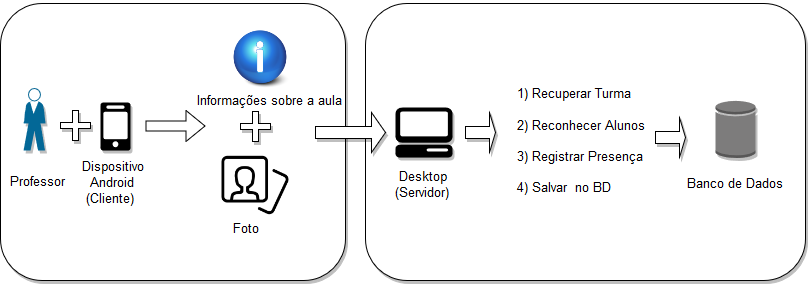
\includegraphics[width=1.0\textwidth]{img/diagramaintro.png}   
	\caption{Estrutura do Sistema}
	\label{fig:figura1}
\end{figure}

\section{Estrutura}
Este trabalho será organizado de acordo com o seguinte formato: O capítulo 1 traz uma breve introdução e contextualização do tema. o capítulo 2 contém os conceitos básicos relacionados à detecção e reconhecimento facial; o capítulo 3 trata da modelagem do sistema; o capítulo 4 aborda a construção do módulo servidor, esse módulo contempla o reconhecimento facial; o capítulo 5 trata do módulo \textit{mobile}, mostrando o aplicativo desenvolvido e o programa que executado no servidor é responsável por receber a fotografia e as informações enviadas pelo professor, como seu desenvolvimento estava intimamente ligado com o aplicativo, optou-se por descrevê-lo nesse capítulo; o capítulo 6 descreve o módulo BD, e é responsável pela criação do esquema no banco de dados, aborda-se ainda a conexão do módulo servidor com o banco de dados, além de se abordar a interface web (servidor web)  para visualização e alteração das papeletas; o capítulo 7 faz a Análise crítica do sistema, e por fim, o capítulo 8 aborda a  conclusão do projeto.
%\begin{itemize}
%\item \textit{Capítulo 2:} Será realizada a discussão sobre os conceitos básicos relacionados a detecção e reconhecimento facial.
%\item \textit{capítulo 3:} Define-se a modelagem do sistema, dividindo-o em módulos. 
%\item \textit{Capítulo 4:} %Novos capitulos pra VC
%\item \textit{Capítulo 5:} %Novos capitulos pra VC
%\item \textit{Capítulo 6:} descrição e explicação do planejamento do projeto.
%\item \textit{Capítulo 7:} expõem a conclusão parcial do projeto.


%\end{itemize}




\chapter{Reconhecimento Facial}
\noindent
O reconhecimento facial desenvolve a tarefa mais importante do projeto, na medida em que ele é o responsável direto pela apuracão de faltas. Essa tarefa possui, basicamente, dois estágios: a detecção facial e o reconhecimento facial propriamente dito. 
\section{Detecção Facial}
Nessa seção, são descritas as especificidades básicas dos algoritmos de detecção facial, representados nesse projeto pelos algoritmos \textit{haarcascade frontal face} e \textit{haarcascade eye}, os quais são componentes da biblioteca de código aberto OpenCV, cujas especificações estão disponíveis na documentação \citep{open2018}, e são utilizados como classificadores para detectar faces e olhos, respectivamente. O principal objetivo desses algoritmos é identificar algum objeto em uma imagem, determinando seu tamanho e localização, que será extraído da imagem e processado de forma a facilitar o reconhecimento.

Esses algoritmos, baseados no trabalho de \citep{Viola2001}, são constituídos por quatro componentes: \textit{Haar-like features}, imagem integral (\textit{Integral Image}), o algoritmo de aprendizado chamado de \textit{Adaboost} e a combinação de classificadores em cascata. As \textit{Haar-like features} (características) são as estruturas utilizadas para identificar objetos em uma imagem. Elas podem ter diferentes formatos e tamanhos e são representadas por figuras retangulares que cobrem uma determinada área da imagem que se deseja analisar. Na figura \ref{fig:figura2} pode-se observar alguns exemplos dessas características:

\begin{figure}[!ht]
	\centering
	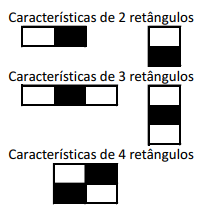
\includegraphics[width=0.3\textwidth]{Haarf.png}   
	\caption{Haar-like Features}
	\label{fig:figura2}
\end{figure}

Os retângulos pretos correspondem a um grupo de \textit{pixels} com tonalidade escura, ao passo que os retângulos brancos correspondem aos \textit{pixels} com tonalidade clara. Cada característica é definida por um valor que é obtido pela diferença entre o somatório das intensidades dos \textit{pixels} contidos na área preta e o somatório dos \textit{pixels} da área branca. Quando este valor é superior a um limiar padronizado, diz-se que a característica está presente na imagem. A figura \ref{fig:figura3} é um exemplo de aplicação desse conceito: há a utilização de uma característica de três retângulos (sendo dois pretos e um branco) para verificar se a imagem contem olhos, isso porque, normalmente, a região dos olhos é mais escura que a região superior do nariz. Em outras palavras, para que a existência de olhos seja detectada é necessário que uma característica com aquele formato específico possua um valor superior ao limiar determinado em treinamento.

\begin{figure}[!ht]
	\centering
	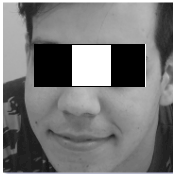
\includegraphics[width=0.3\textwidth]{exemplo_haar_features.png}   
	\caption{Exemplo de Haar-like Features}
	\label{fig:figura3}
\end{figure}

A Imagem Integral é uma técnica desenvolvida por \citep{Viola2001} para agilizar o cálculo das características. Para tanto, cria-se uma imagem intermediária tal que o valor de qualquer \textit{pixel} na posição (x,y) é dado pelo somatório dele com todos os \textit{pixels} localizados acima e a esquerda dele. Dessa forma, não é necessário acessar o valor de cada \textit{pixel} para calcular o valor de uma área. A figura \ref{fig:figura4} ilustra o funcionamento dessa técnica: nesse exemplo uma imagem está sendo representada por uma matriz 4x4, a qual contém uma região destacada cujo valor se deseja obter, note que o valor da soma dos \textit{pixels} dessa área já está definido na imagem integral, na última posição que define a área escolhida (sempre localizado no canto inferior direito).

\begin{figure}[!ht]
	\centering
	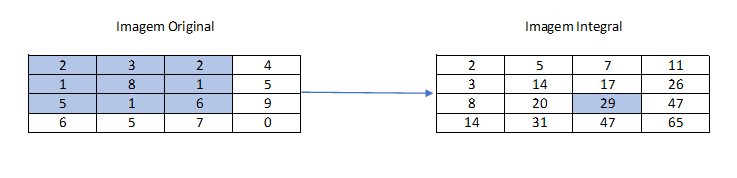
\includegraphics[width=1.0\textwidth]{imagem_integral.png}   
	\caption{Exemplo de Imagem Integral}
	\label{fig:figura4}
\end{figure}

Foi exposto anteriormente que a associação de características a objetos está condicionada a um treinamento. Essa tarefa é realizada pelo algoritmo de aprendizado de máquina supervisionado \textit{Adaboost}, cujo objetivo é construir um conjunto de classificadores simples, sendo cada um composto por apenas uma característica importante para a detecção do objeto, \citep{Viola2001}. Essa tarefa é importante porque em uma imagem existe uma grande quantidade de características (\textit{Haar-like features}) e, por isso, encontrar os tipos de características que melhor representam o objeto alvo economiza o esforço de analisar todas as demais. A \textit{Haar-like feature} da figura \ref{fig:figura3} é um exemplo de característica que compõe um classificador simples, pois ela sozinha não define uma face, mas a sua ausência já descarta a possibilidade de ser um rosto. Assim, o treinamento desse algoritmo consiste, segundo \citep{open2018}, na exposição de algumas centenas de amostras de um objeto específico, como um rosto ou um carro, chamados de exemplos positivos, os quais são formatados para terem as mesmas dimensões para só então compará-los com imagens arbitrárias de outros objetos de mesmas dimensões, chamados de exemplos negativos. Dos exemplos positivos, portanto, são definidos os classificadores (características e limiares).

Terminado o treinamento, é possível aplicar o classificador numa imagem de entrada. Quando o valor do conjunto de características que compõem o classificador é superior ao seu limiar, este atribui o valor 1 a imagem, o que indica que o objeto alvo está presente na imagem, caso contrário atribui 0, \citep{open2018}. Na detecção facial, esse processo ocorre diversas vezes por meio da combinação dos classificadores em cascata, que consiste no encadeamento de vários classificadores simples aplicados em sequência em uma imagem, que crescem em complexidade a cada iteração,  até que essa região seja rejeitada, por algum classificador, ou aprovada em todos os classificadores, \citep{open2018}. Quando a imagem é rejeitada por algum classificador simples, o processo encerra sem que os outros classificadores sejam aplicados. Esse procedimento aumenta drasticamente o desempenho e a precisão da detecção do objeto, pois as imagens indesejadas são eliminadas nas iterações iniciais, envolvendo menor processamento, sobrando para os classificadores mais complexos apenas aquelas com alta probabilidade de ser o objeto procurado.

Dessa forma, o papel a ser desenvolvido pelos algoritmos citados no início dessa seção é apoiar o reconhecimento facial, a partir da detecção de faces em imagens captadas por uma câmera fotográfica, as quais serão processadas e armazenadas para posterior análise dos algoritmos de reconhecimento facial que serão o objeto da seção seguinte.
\newpage
\section{Algoritmos de Reconhecimento Facial}
\noindent
Concluída a etapa de detecção facial, tem-se como produto a imagem da face já redimensionada, transformada para a escala de cinza e recortada da imagem original, esse processo é ilustrado na figura \ref{fig:figura25}, em (b) ocorre a transformação para a escala cinza (o retângulo vermelho é apenas uma abstração utilizada para representar a borda do que se irá recortar), e em (c) o recorte propriamente dito. A partir daí começa a etapa de reconhecimento que possui, basicamente, duas modalidades: autenticação e identificação. A primeira consiste em uma comparação 1 X 1 entre a imagem de entrada com a imagem da pessoa a ser autenticada. A segunda consiste em uma comparação 1 X N na qual a entrada é comparada com todas as imagens de um determinado conjunto para determinar se alguma pessoa do conjunto corresponde à entrada \citep{tdc2018}. No processo de apuração de faltas, convém utilizar apenas a modalidade de identificação.

\begin{figure}[!ht]
	\centering
	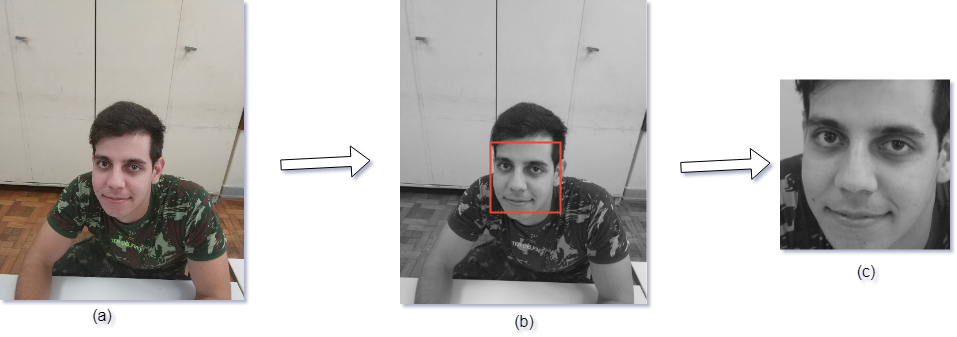
\includegraphics[width=1\textwidth]{processoRecorte.png}   
	\caption{Processo de recorte}
	\label{fig:figura25}
\end{figure}

Para o cumprimento da tarefa de reconhecimento facial, a biblioteca OpenCV  oferece três algoritmos: \textit{Eigenfaces}, \textit{Fischerfaces} e o LBPH. Por fazerem parte de uma biblioteca de código aberto, esses algoritmos são gratuitos para uso e esse fato contribuiu para a sua popularização, tendo como resultado o seu uso frequente em trabalhos científicos. Outro fator motivador para o emprego desses algoritmos é o seu bom desempenho, pois quando comparado ao MATLAB, que também pode ser utilizado para essa função, o OpenCV se destaca por usar menos memória e ser mais rápido que o seu concorrente, pois pode processar 30 quadros por segundo, enquanto o MATLAB executa de 3 a 4 quadros por segundo \citep{Kriti2018}. 

Quanto aos algoritmos, observou-se que em trabalhos científicos cujo objetivo é realizar o controle de faltas por meio de reconhecimento facial, o LBPH é apontado como a melhor opção dentre os três. Isso porque os algoritmos que utilizam as técnicas de PCA e LDA (Eigenfaces e Fisherfaces, respectivamente) para o reconhecimento facial apresentam dificuldades para superar problemas como a variação de: dimensionamento, iluminação, rotação e oclusão \citep{varun2018}. O trabalho de \citep{Kriti2018} também indica a superioridade do LBPH, o qual é classificado como o algoritmo mais eficiente e preciso, do OpenCV, para a tarefa de reconhecimento, após fazer um teste de desempenho comparando os três algoritmos. Esse teste também apontou a invariância à iluminação do LBPH, especialmente quando aplicado em imagens na escala de cinza, bem como a interferência mínima de ruídos. 

%Devido a essa robustez a variações, o LBPH foi o algoritmo escolhido para o desenvolvimento do presente projeto.


\subsection{Local Binary Patterns Histograms}
Descrito inicialmente em 1994, a operação LBP ficou conhecida como uma poderosa ferramenta de classificação de texturas, a qual teve a sua performance de detecção melhorada consideravelmente quando passou a ser combinada com histogramas de gradientes orientados \citep{tdc2018}. Com o uso dos histogramas o algoritmo é chamado de LBPH. O seu funcionamento possui 4 fases: treinamento do algoritmo, aplicação da operação LBP, extração de histogramas e reconhecimento de face.

O treinamento funciona de forma semelhante ao que foi descrito nos algoritmos de detecção, porém as imagens que compõem a base de dados são das pessoas a serem reconhecidas. Além disso, cada foto do arquivo precisa de uma identificação, podendo ser um número ou o nome da pessoa, que dever ser a mesma para todas as fotos. Isso é feito para que o algoritmo associe a uma mesma identificação as diversas expressões que uma pessoa possa fazer, aumentando, portanto, a probabilidade de reconhecimento.

A forma básica da operação LBP consiste em classificar os \textit{pixels} de uma imagem da seguinte maneira: a partir de uma região contendo 9 \textit{pixels}, que são representados por uma matriz 3 X 3, com cada \textit{pixel} assumindo um valor, correspondente a intensidade de cor, entre 0 e 255 (correspondentes aos tons de cinza). Em seguida usa-se o valor central da matriz como limiar para definir um novo valor, agora binário, para os outros 8 vizinhos. Caso o valor do \textit{pixel} vizinho seja menor que o valor do limiar, atribui-se o valor 0, caso contrário o valor é 1. O próximo passo é concatenar os valores para ter uma sequência binária (daí o nome padrão binário local), que é convertida para um número decimal que passa a representar o conjunto de \textit{pixels}, \citep{tdc2018}. A figura \ref{fig:figura6} ilustra esse processo. A forma mais genérica da operação LBP usa vizinhanças circulares, figura \ref{fig:figura7} , as quais podem abranger qualquer quantidade de vizinhos com a variação do raio, definidos pelo usuário, por meio de uma interpolação bilinear dos valores dos \textit{pixels} \citep{Timo2006}.

%Com relação ao funcionamento do algoritmo, inicia-se a partir de uma imagem na escala de cinza,
\begin{figure}[!ht]
	\centering
	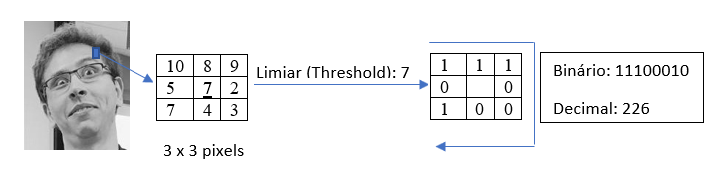
\includegraphics[width=1.0\textwidth]{lbpV1.png}   
	\caption{Operação LBP}
	\label{fig:figura6}
\end{figure}

\begin{figure}[!ht]
	\centering
	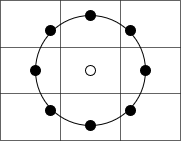
\includegraphics[width=0.25\textwidth]{vizicircular.png}   
	\caption{Operação LBP - vizinhança circular}
	\label{fig:figura7}
\end{figure}

O procedimento seguinte é a extração dos histogramas, que consiste em agrupar os valores dos \textit{pixels }classificados pela operação LBP, de forma que para cada região da imagem haverá um histograma contendo a quantidade de ocorrências de cada tom de cinza presente. Essas regiões que dividem a imagem são chamadas de \textit{grids}, pois têm o mesmo aspecto de uma grade, e podem ter qualquer formatação quanto a quantidade de linhas e colunas: nas linguagens de programação os parâmetros que definem a quantidade de \textit{grids} são \textit{Grid x} e \textit{Grid y}. Os histogramas extraídos de cada \textit{grid} representam características locais, contendo 256 posições (de 0 a 255) relativas aos diversos tons de cinza. Em seguida, todos os histogramas locais são concatenados, gerando um histograma global que representa as características da imagem principal, conforme pode ser vista na figura \ref{fig:figura8} , \citep{Timo2006}. Dessa forma, para uma imagem de 9 x 9 \textit{grids}, tem-se um histograma de 20.736 posições (9x9x256). \newpage

\begin{figure}[!ht]
	\centering
	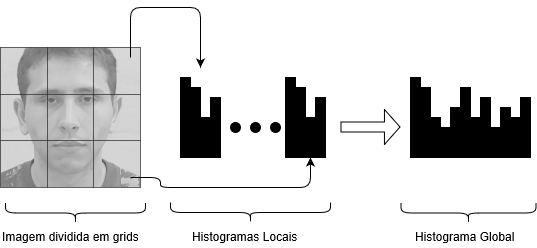
\includegraphics[width=0.7\textwidth]{lbphC.png}   
	\caption{Extração de Histogramas}
	\label{fig:figura8}
\end{figure}

O reconhecimento facial se dá, portanto, pela comparação entre os histogramas globais: da imagem de entrada com as imagens do conjunto de treino. O parâmetro de comparação utilizado é a distância entre os vetores de características, que são as estruturas de dados usadas para armazenar a informação dos histogramas. Na implementação do LBPH do OpenCV existem 4 métodos para o cálculo dessa distância: a distribuição qui-quadrado, a distância euclidiana, a distância euclidiana normalizada ou a fórmula do valor absoluto \citep{open2018}. Após o cálculo das distâncias entre a imagem de entrada e as imagens do banco de dados, o algoritmo retorna a identificação da imagem que apresenta a menor distância em relação à imagem de entrada. %$D = \sqrt[]{\sum_{i=1}^{n}(hist1_{i} - hist2_{i})^{2}}$


\chapter{Modelagem do Sistema}
\noindent
Este capítulo tem o objetivo de abordar a modelagem proposta para o sistema. Vale destacar que o sistema se propõe a não somente realizar o reconhecimento facial, como também permitir o armazenamento persistente das faltas apuradas, permitir a correção de eventuais erros de apuração e possuir mecanismos de consultas das faltas. O escopo do projeto abrange a apuração e o registro das faltas, sem incluir, portanto, a apuração de pontos perdidos.

\section{Levantamento de requisitos}
\noindent
O levantamento de requisitos é uma importante atividade para se entender o problema. Segundo \citep{bezerra}, essa etapa tem a finalidade de que desenvolvedores e usuários compartilhem da mesma visão do problema a ser solucionado. Buscou-se realizar uma série de procedimentos com a finalidade de levantar os requisitos funcionais e não-funcionais aqui expostos. Dentre as técnicas adotadas merecem destaque a análise de documentos, \textit{Brainstorming} e entrevistas informais.

\subsection{Requisitos Funcionais} 

Segundo \citep{bezerra} esse tipo de requisito está ligado às funcionalidades do sistema.  A seguir apresenta-se o resultado desse levantamento.

\begin{itemize}
\item RF01 - Apurar falta: O sistema deve apurar as faltas de um determinado tempo de aula em uma data, disciplina, para uma turma, usando o reconhecimento facial em uma fotografia da turma. As fotos devem ser tiradas por um dispositivo móvel com câmera ou selecionadas de sua galeria. Deve-se reconhecer várias faces em uma mesma fotografia, isso é, a fotografia é da turma e não individual. O professor deve poder enviar uma ou mais fotografias em um único tempo de aula, em operações de envio distintas. Assim ao enviar uma fotografia, e verificar que nem todos os alunos presentes receberam a presença, ele poderia enviar uma fotografia em adição à apuração anterior. Isso também ajuda, para os casos em que a turma não pode ser enquadrada em uma única fotografia. As informações referentes a data, isso é, dia, mês e ano devem ser extraídas do servidor; 

\item RF02 - Verificar lista de presença : Um aluno, coordenador ou professor deve ser capaz de  exibir a lista de presença referente a um determinado tempo de aula, de um determinado dia para uma turma específica; 
\item RF03 - Editar lista de presença : O professor deve ser capaz de alterar as faltas de um tempo de aula, isso permite que ele corrija eventuais erros na apuração de faltas que usou o reconhecimento facial; e 
\item RF04 - Armazenar fotografia : Deve-se armazenar a fotografia com sua apuração no servidor, em uma pasta específica para isso, permitindo uma eventual auditoria.
\end{itemize}

\subsection{Requisitos Não-Funcionais}
Tratam sobre características do sistema, \citep{bezerra} elenca alguns tipos como confiabilidade, desempenho, portabilidade, segurança e usabilidade. A seguir apresenta-se os requisitos não-funcionais levantados.

\begin{itemize}
%\item RN01 - O índice de erro no reconhecimento facial deve ser inferior a 50\%. Considera-se como erro, apenas os casos em que a face da pessoa X é reconhecida como sendo da pessoa Y. A classificação como desconhecida não caracteriza um erro de reconhecimento;

\item RN01 - O Sistema deve apresentar interface com o usuário “Professor” compatível com o  sistema Android; 

\item RN02 - O banco de dados, no qual se fará o armazenamento persistente, deve ser PostgreSQL;

\item RN03 - As tarefas de captura de foto, reconhecimento facial e armazenamento de registros devem ser feitas em módulos distintos; e

\item RN04 - Um professor deve ser capaz de utilizar o sistema após um treinamento de 15 minutos.

\end{itemize}


\section{Casos de uso}
\noindent
Segundo \citep{bezerra}, o modelo de casos de uso  consiste em um refinamento dos requisitos funcionais. Acrescenta que os casos de uso tratam sobre funcionalidades externas do sistema, assim não se abordam mecanismos internos. Assim, com base nos requisitos funcionais apresentados no tópico 3.1.1, tem-se a figura \ref{fig:figura03} que traz o diagrama de casos de uso. Vale destacar que o RF04 foi incorporado ao RF01 gerando um único caso de uso, isso se explica pois o armazenamento da imagem só ocorre posteriormente à apuração das faltas. Os atores \textbf{professor} e \textbf{usuário} são apresentados utilizando-se  o relacionamento de generalização entre atores. Além disso usuário também comporta os alunos e os coordenadores. 

%altearar figura
\begin{figure}[!ht]
	\centering
	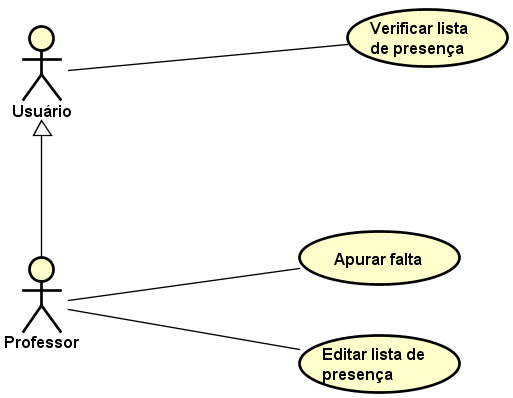
\includegraphics[width=0.8\textwidth]{dcu.png}   
	\caption{Diagrama de casos de uso}
	\label{fig:figura03}
\end{figure}
Nas subseções seguintes é feito o detalhamento dos casos de uso \textbf{apurar falta}, \textbf{editar lista de presença}, \textbf{verificar lista de presença}.


\subsection{Apurar Falta} 
\noindent
Identificador e nome: UC-01. Apurar falta.

Sumário: O ator utiliza esta função para apurar as faltas de um tempo de aula específico, através de uma fotografia da turma.

Ator Principal: Professor.

Pré-condição: O ator começa um tempo de aula e inicia o aplicativo Android Tchau Papeletas.

Fluxo Principal:

1- O ator solicita a função apurar faltas.

2- O sistema apresenta os campos código e tempo de aula para preenchimento e seleção, respectivamente. Além do campo para a fotografia.

3- O ator preenche com o código, formado pelo nome da turma + '.' + nome da matéria, e seleciona o tempo de aula.

4- O ator seleciona uma imagem previamente existente  ou abre a câmera do dispositivo e fotografa a turma.

5- O ator clica em enviar.

6- O sistema acusa \textit{upload} realizado com sucesso.

Pós-condição: A apuração de faltas daquele tempo de aula foi realizada e registrada no banco de dados, uma imagem com as faces identificadas foi salva no servidor.


\subsection{Editar Lista de presença} 
\noindent
Identificador e nome: UC-02. Editar Lista de presença.


Sumário: O ator utiliza esta função para alterar as faltas apuradas no UC-01. Permitindo assim, correções na apuração pelo reconhecimento facial.

Ator Principal: Professor

Pré-condição: Uma apuração utilizando o reconhecimento facial já foi realizada para aquele tempo de aula.

Fluxo Principal:

1- O ator solicita a função editar lista de presença.

2- O sistema apresenta os campos código e tempo de aula, além de dia, mês e ano.

3- O ator preenche os campo nome da turma, nome da matéria, tempo de aula e a data, formada por dia, mês e ano.

4- O sistema exibe a papeleta de faltas preenchida, com as faltas apuradas pelo UC-01. Essa papeleta contém em seu cabeçalho a disciplina, o tempo de aula, data (dia, mês e ano) e turma. Em seu corpo, o código do aluno (matrícula), o nome do aluno e a presença ou ausência do aluno. Esse último campo é editável. Na parte inferior um botão de confirmar alterações.

5- O ator realiza as alterações de presença que julgar ser necessário. Ao final, pressiona o botão  de confirmar alterações.

6- O sistema exibe uma mensagem de alerta, pedindo uma nova confirmação. 

7- O ator confirma a operação.

8- O sistema acusa atualização realizada com sucesso.

Pós-condição: A apuração de faltas daquele tempo de aula foi alterada e registrada no banco de dados.


\subsection{Verificar Lista de Presença} 
\noindent
Identificador e nome: UC-03. Verificar Lista de Presença.

Sumário: O ator utiliza esta função com a finalidade de verificar as faltas de um tempo de aula específico. Seria similar a observar a papeleta de faltas preenchida.

Ator Principal: Aluno, Coordenador  e Professor

Pré-condição: Uma apuração utilizando o reconhecimento facial já foi realizada para aquele tempo de aula.

Fluxo Principal:

1- O ator solicita a função verificar lista de presença.

2- O sistema apresenta os campos código e tempo de aula, além de dia, mês e ano.

3- O ator preenche os campo nome da turma, nome da matéria, tempo de aula e a data, formada por dia, mês e ano.

4- O sistema exibe a papeleta de faltas preenchida, com as faltas apuradas pelo UC-01 e possivelmente alteradas pelo UC-02 . Essa papeleta contém em seu cabeçalho a disciplina, o tempo de aula, data (dia, mês e ano) e turma. Em seu corpo, o código do aluno (matrícula), o nome do aluno e a presença ou ausência do aluno.

Pós-condição: O sistema permanece inalterado.




\section{Conceito Geral do Sistema}
\noindent
A partir das etapas anteriores, pode-se depreender o conceito geral do sistema e como ele será trabalhado. Segundo \citep{engenhariasoftware} a engenharia de \textit{software} tem como objetivo principal a entrega do \textit{software} em tempo hábil, com alta qualidade e que atenda aquilo que lhe foi requisitado. Para atender esse objetivo, \citep{engenhariasoftware} elenca uma série de princípios, dentre os quais, se destaca o conhecido princípio dividir para conquistar, que como o nome sugere se trata de subdividir o problema em partes menores. Posteriormente, os mencionados autores depreendem desse princípio um outro, que é o de construir \textit{softwares}  apresentando o que chamam de modularidade efetiva. Sobre isso, afirmam que: "cada módulo deve se concentrar exclusivamente em um aspecto bem restrito do sistema – deve ser coeso em sua função e/ou apresentar conteúdo bem preciso"\ \cite[p. 109]{engenhariasoftware}.
% citar página 109 do engenhariasoftware

A modularidade permite que um módulo seja substituído por outro, sem que se tenha de alterar o sistema como um todo, além disso facilita a manutenção, uma vez que cada módulo tem um propósito bem definido. O sistema se dividirá em 3 módulos, a saber:

\begin{itemize}
\item \textit{Módulo Servidor:} esse é o responsável por receber a fotografia tirada da turma, assim como os dados como turma, dia, hora e matéria. Ele deverá detectar as faces na fotografia e depois, utilizando o algoritmo escolhido, identificar cada uma delas. Para cada face reconhecida deve-se atribuir a presença, a qual será enviada para o armazenamento persistente;
\item \textit{Módulo Mobile:} ele permitirá que o professor fotografe a turma, insira os dados mencionados acima, e encaminhe para o servidor, oferecendo ao professor uma interface amigável. Além disso, ele permitirá que o professor visualize a papeleta digital após a apuração e a corrija, se for o caso. Para tal, será projetado para o sistema \textit{Android}; e
\item \textit{Módulo BD:} é onde se dará o armazenamento persistente das informações. Ele terá as informações sobre os alunos, como nome, turma, matrícula, disciplinas daquela turma, e é claro a presença/falta no tempo de aula.
\end{itemize}

%A figura \ref{fig:figura04} mostra o funcionamento do sistema descrito acima:

%\begin{figure}[!ht]
%	\centering
%	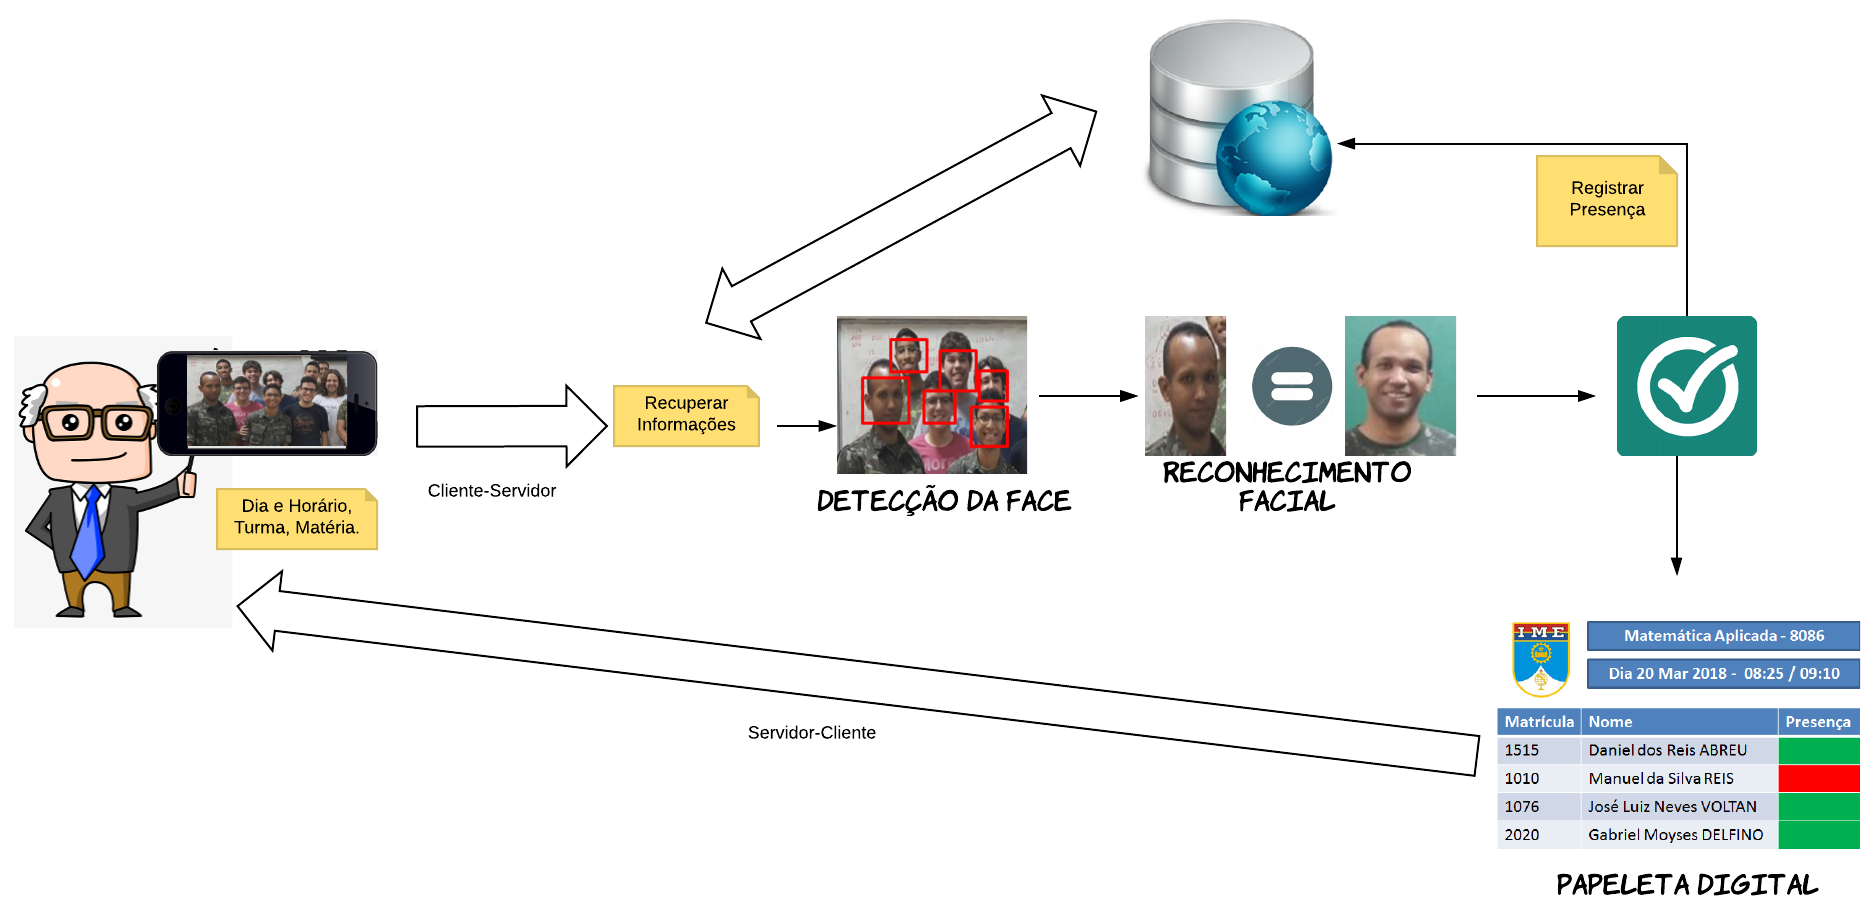
\includegraphics[width=1\textwidth]{esquema.png}   
%	\caption{Modelo de funcionamento geral do sistema}
%	\label{fig:figura04}
%\end{figure}

Pode-se ainda detalhar as atividades envolvidas no processo de reconhecimento facial através de um diagrama de atividades, conforme a figura \ref{fig:figura05}. 

\begin{figure}[!ht]
	\centering
	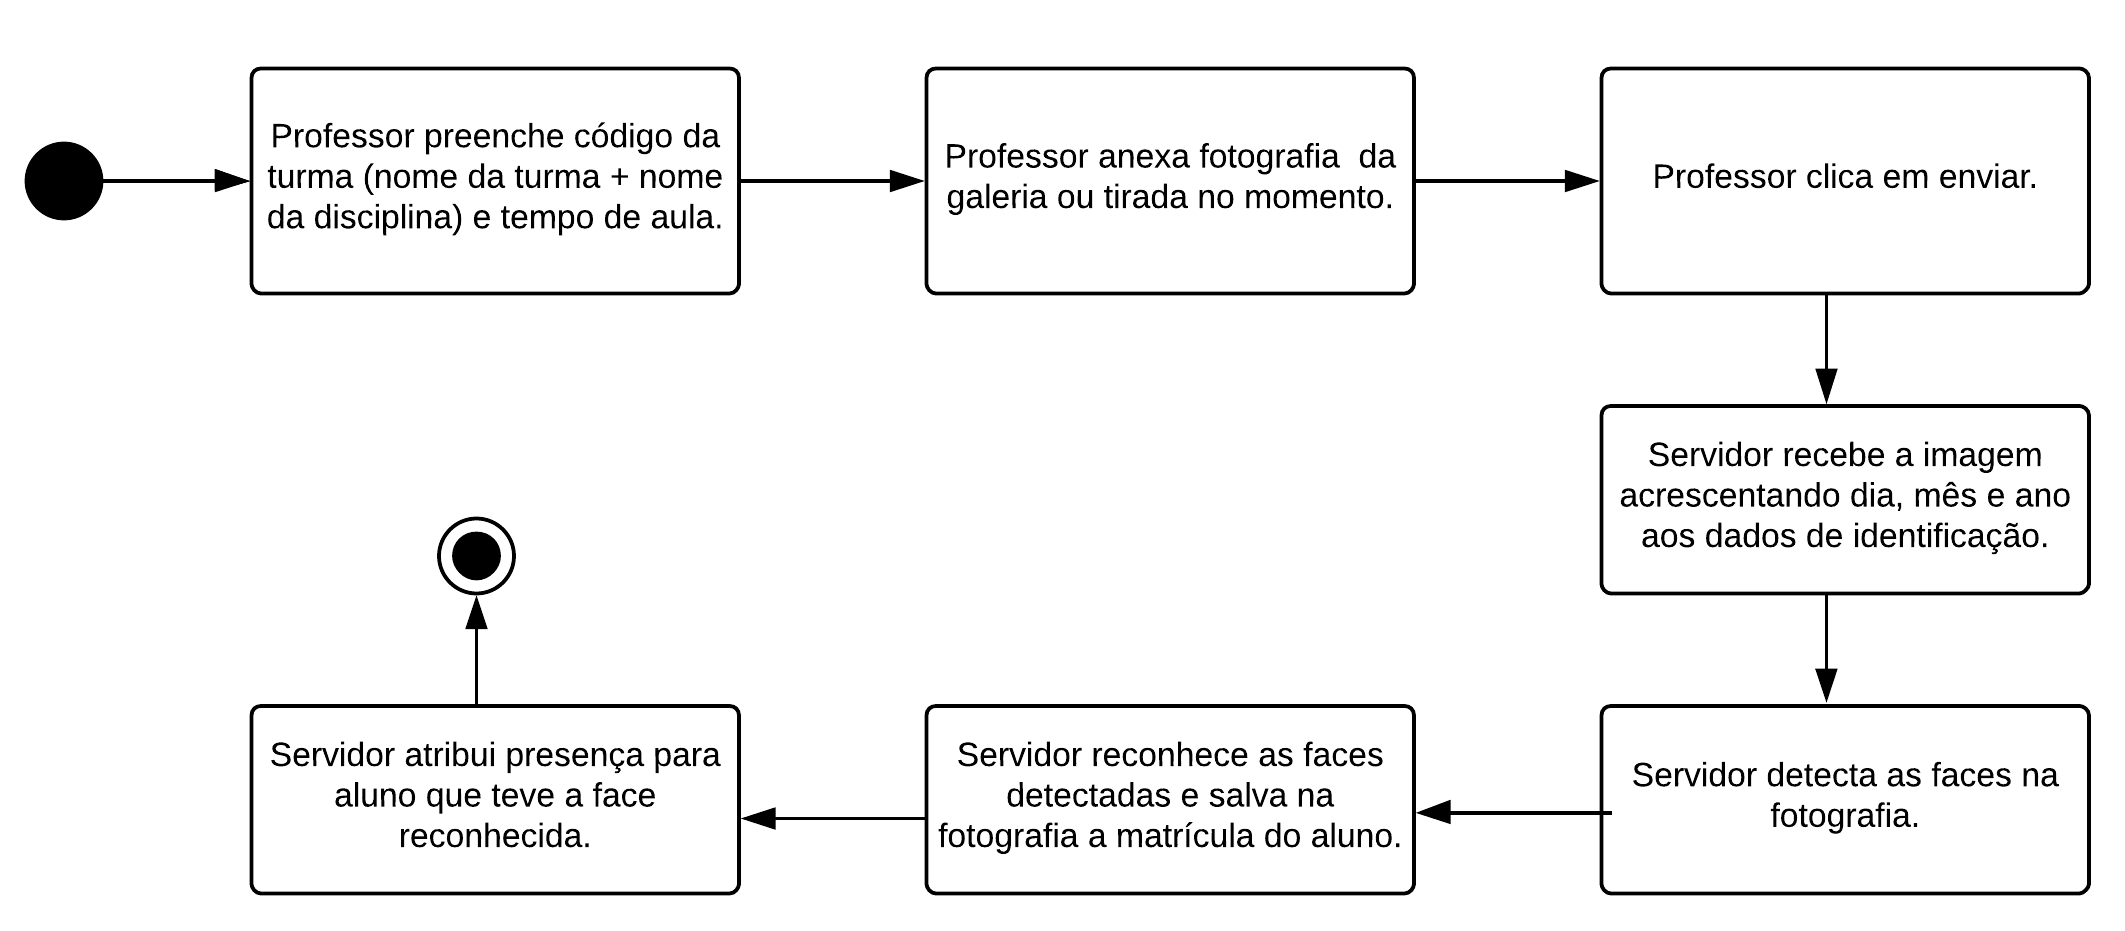
\includegraphics[width=1\textwidth]{diagativigeral.png}   
	\caption{Diagrama de atividades para o reconhecimento facial}
	\label{fig:figura05}
\end{figure}

%Os módulos devem se comunicar de maneira eficiente, permitindo que o sistema atinja seu objetivo.


\chapter{Módulo Servidor}
\noindent
Este capítulo tem o objetivo de abordar o 1º módulo desenvolvido para atender o objetivo proposto, o módulo do servidor. De maneira geral, como já mencionado, ele é o responsável por analisar a fotografia da turma, assim como os dados pertinentes. Ele deverá detectar as faces na fotografia e depois, utilizando o algoritmo LBPH, identificar cada uma delas. Para cada face reconhecida deve-se atribuir a presença, a qual será enviada para o armazenamento persistente, o banco de dados PostgreSQL. Ele está relacionado aos requisitos funcionais \textit{RF01 - Apurar falta} e   \textit{RF04 - Armazenar fotografia}. Ele atende ao caso de uso \textit{UC-01 Apurar falta}. Optou-se por abordar o processo de envio e recebimento das fotografias e dados, no módulo \textit{mobile}. Assim a atividade do módulo servidor se inicia ao detectar uma fotografia na pasta faltas.  

\section{Conceito Geral do módulo}
\noindent
 Segundo \citep{Arubas} o reconhecimento compara a face (desconhecida) que se quer reconhecer com um conjunto de treinamento de faces conhecidas. No conjunto de treinamento, são fornecidas as faces e a qual pessoa elas pertencem. Quando é solicitado ao algoritmo que reconheça alguma face desconhecida, ele usa o conjunto de treinamento para fazer o reconhecimento. Ele destaca ainda que, o LBPH analisa cada rosto no conjunto de treinamento de forma individual e independente. 
 
O presente projeto utilizou a biblioteca OpenCV, onde se explorou os algoritmos \textit{HaarCascade}, detecção de olhos e o de detecção de faces, para a detecção com maior grau de certeza das faces e o LBPH para o reconhecimento da face. O OpenCV, conforme \citep{opengeral2018}, é uma biblioteca gratuita para uso no meio acadêmico e comercial. Ela é voltada para visão computacional e aprendizado de máquina, tendo sido escrita primeiramente em C++. Possui interfaces nas linguagens C++, Python, Java e MATLAB.

Optou-se por utilizar a interface na linguagem Python, devido as características da linguagem, tais como facilidade de leitura e compreensão, além da fácil manutenção. Nesse sentido, \citep{pythonLTC} diz que Python é uma linguagem caracterizada como sendo de uso geral, que foi idealizada para fazer com que os programas sejam muito legíveis, isso é, priorizou-se a legibilidade. Além disso, Python também possui inúmeras  bibliotecas,  isso torna possível a escrita de aplicações sofisticadas, mas com aparência simples. Pelas razões apresentadas, o mencionado autor conclui que "Python tornou-se uma linguagem de desenvolvimento de aplicações popular e também uma preferência como “primeira” linguagem de programação"\ \cite[p. 22]{pythonLTC}. 

Vale destacar nesse momento uma particularidade do Python. Conforme \citep{pythonLTC}, a versão 2 não é compatível com a  3. Isso significa que um programa escrito em Python 2, provavelmente, não irá funcionar usando um interpretador de Python 3. \citep{pythonLTC} considera que a versão 3 apresenta uma maior consistência que a 2. Nesse aspecto, optou-se por utilizar o Python 3.6.3, o qual foi, segundo \citep{python_org}, lançado em 03 de outubro de 2017. 
 
Quanto ao OpenCV, a versão escolhida foi a 3.4.2. Essas considerações sobre as versões se justificam devido ao fato de que por vezes, métodos e formas de trabalho idealizadas para uma determinada versão, acabam sendo modificados em versões seguintes. Justamente para evitar esse tipo de problema, optou-se por utilizar uma única versão ao longo do desenvolvimento do trabalho.
 
 
\section{Etapas pré-reconhecimento}
\noindent 
Antes de realizar o reconhecimento facial, faz-se necessário realizar o treinamento, isso é, gerar o conhecimento sobre a turma, gera-se um arquivo que concatene as informações extraídas de cada uma das fotografias, mantendo a identificação (a quem pertence) de cada uma das faces aprendidas. Para isso, segue-se as seguintes etapas ilustradas na figura \ref{fig:figura50}

\begin{figure}[!ht]
	\centering
	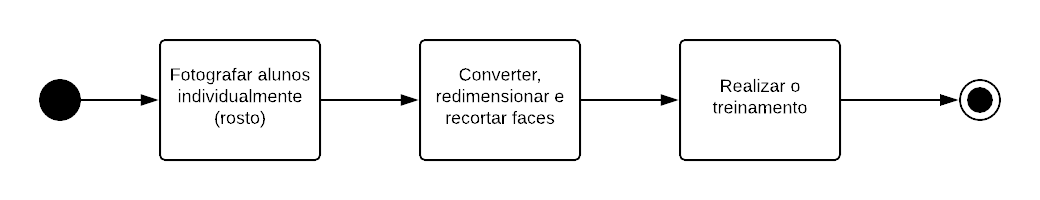
\includegraphics[width=1\textwidth]{UML_cap_mod1.png}   
	\caption{Diagrama de atividades da fase pré-reconhecimento}
	\label{fig:figura50}
\end{figure}

Na primeira etapa deve-se fotografar o aluno de forma individual, com uma grande variedade de expressões, ângulos de fotografia e incidência de luz. Essa é uma etapa muito importante, pois essas imagens formarão a base de conhecimento (imagens a serem treinadas). 

Depois disso, utiliza-se o artefato responsável pela conversão, desenvolvido ao longo do módulo servidor. Ele faz com que a fotografia seja transformada em uma escala cinza, ocorra a detecção da face utilizando o \textit{haarcascade frontal face}, depois disso, essa região é verificada com o \textit{haarcascade eye}, a fim de eliminar-se resultados falso-positivos, isso é, eliminar a situação em que um objeto é reconhecido erroneamente como uma face. Por fim ocorre o recorte dessa face já na escala cinza e em um mesmo tamanho (720x720). Nesse ponto vale destacar que não são todas as fotografias que irão gerar faces válidas, uma vez que o \textit{haarcascade frontal face} e o \textit{haarcascade eye} podem não detectar nenhuma face, mesmo havendo. O programa recebe do usuário o nome da turma, e converte todas imagens contidas na pasta com esse nome. Oferece ainda ao usuário a opção de escolher se deseja exibir cada uma das fotografias antes da converter ou não. Ao final da conversão das imagens de cada aluno, exibe-se a quantidade de imagens lidas, e a quantidade de faces reconhecidas, isso é, que foram de fato aproveitadas e geraram uma nova imagem. A figura \ref{fig:figura51} ilustra esse procedimento, mostrando além do nome do arquivo, sua luminosidade. 

\begin{figure}[!ht]
	\centering
	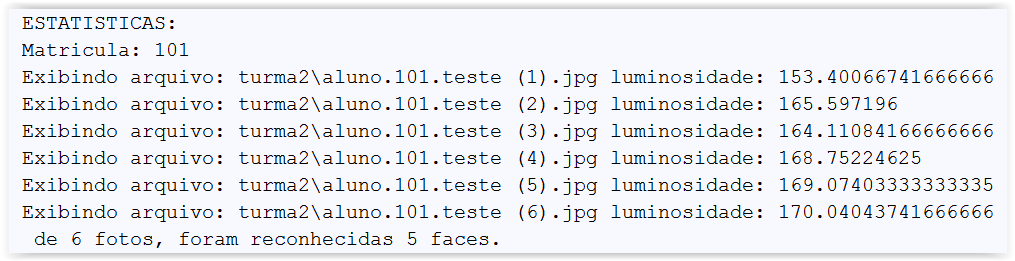
\includegraphics[width=0.9\textwidth]{conversor_saida_estatistica.PNG}   
	\caption{Informações estatísticas exibidas ao final do processo conversor}
	\label{fig:figura51}
\end{figure}

Uma padronização adotada foi o nome dado às fotografias, optou-se por utilizar a seguinte concatenação de nomes "aluno" + "." + o número da matrícula do aluno + "." + nome da turma + " (" + número da fotografia + ").jpg", por exemplo: "aluno.101.comp18 (1).jpg", na figura \ref{fig:figura51} o nome  de turma usado foi "teste". Essa padronização de nomenclatura facilita o processo de codificação e foi utilizada para armazenar o número da foto e a matrícula do aluno. As imagens de alunos de uma mesma turma foram agrupadas em uma mesma pasta. A figura \ref{fig:figura52} ilustra um exemplo de entrada e saída do procedimento descrito acima. Ao final dessa etapa, tem-se as imagens já convertidas, redimensionadas e recortadas. 

\begin{figure}[!ht]
	\centering
	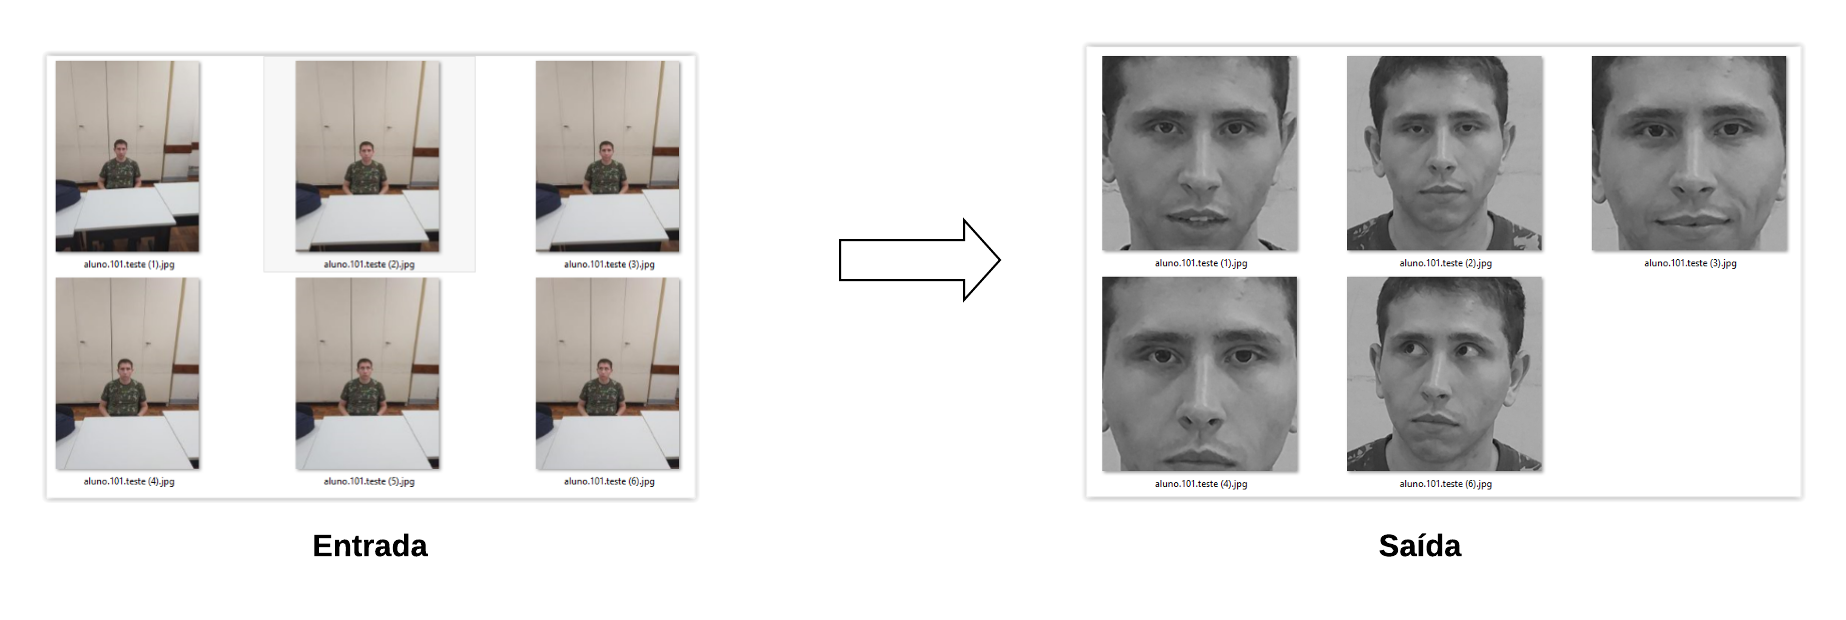
\includegraphics[width=1.0\textwidth]{entrada-conversor-saida.png}   
	\caption{Entrada e saída do conversor}
	\label{fig:figura52}
\end{figure}


\subsection{O treinamento e seus parâmetros}
\noindent
Na etapa seguinte gera-se o arquivo com as informações extraídas das faces, usando-se a metodologia do LBPH, anteriormente apresentada. Assim, através do artefato, desenvolvido ao longo do módulo servidor, "criador\_de\_inteligencia"\ irá se gerar o arquivo de treinamento. Esse é o primeiro momento que o algoritmo LBPH é de fato empregado. Ao se invocar o método \textit{LBPHFaceRecognizer\_create}, tem-se de escolher alguns valores para determinados parâmetros. Quando explicou-se sobre o algoritmo LBPH, eles foram detalhados. São eles:
\textit{radius, neighbors, grid\_x, grid\_y, threshold} 

O parâmetro \textit{radius}, segundo \citep{openlbph2018}, consiste no raio usado para construir o Padrão Binário Local Circular. Raios maiores, tornam mais suaves as imagens, porém, carregam mais informações espaciais. 

Para o parâmetro \textit{neighbors}, \citep{openlbph2018} explica que quanto maior o valor usado para a quantidade de vizinhos, maior será o gasto computacional, ela sugere o uso do valor 8. Esse valor corresponde a uma matriz 3X3, onde pode-se pensar no elemento central, isso é, elemento na linha 2 e coluna 2, como sendo o elemento a ser analisado. Os demais elementos dessa matriz, seriam os vizinhos utilizados. 

Já para o parâmetro \textit{grid\_x} e \textit{grid\_y}, número de células na horizontal e vertical respectivamente, apesar de \citep{openlbph2018} explicar que muitas publicações sugerem o uso do valor 8, os testes realizados no presente projeto obtiveram melhores resultados com o valor 12.

Para melhor escolher os valores a serem utilizados para \textit{neighbors}, \textit{grid\_x} e \textit{grid\_y} realizou-se alguns testes. Utilizou-se o banco de imagens disponibilizado pela Universidade de Yale. \citep{yales} explica que esse banco contém 165 imagens em escala cinza, de 15 pessoas diferentes, havendo portanto 11 imagens por pessoa. Essas imagens variam as expressões da face e condições de iluminação. Além disso, \citep{yales} esclarece que o banco de imagens está disponível publicamente para uso que não seja comercial. As imagens foram convertidas para o formato jpg, por questões de compatibilidade com a biblioteca OpenCV. Os testes consistiram em variando os parâmetros \textit{neighbors}, \textit{grid\_x} e \textit{grid\_y} verificar o índice de acerto no reconhecimento facial. 

Sobre os testes, foram escolhidas 2 imagens de cada pessoa para serem reconhecidas, o que totaliza 30 fotografias. As imagens restantes, isso é, 9 imagens por pessoa, foram utilizadas no treinamento. Como saída do teste, obteve-se a Tabela \ref{tab:tabela1}, nela X e Y referem-se respectivamente aos valores utilizados em \textit{grid\_x} e \textit{grid\_y},  a coluna acertos é exibida em percentagem, já tamanho refere-se ao arquivo gerado pelo treinamento em megabytes, tempo 1 e tempo 2 foram obtidos em segundos e referem-se ao gasto no treinamento, e o total nos reconhecimentos, respectivamente. Por fim  distância refere-se ao somatório das distâncias entre as imagens em análise (faces a serem reconhecidas) e as imagens que mais se aproximam delas. Vale destacar, que em virtude da apuração de tempo, os testes foram repetidos 5 vezes e o tempo mostrado trata-se de uma média aritmética.

Nesses testes, adotou-se o parâmetro \textit{threshold}, no valor de 1000, nos próximos parágrafos serão feitos mais comentários sobre isso. O que vale destacar é que esse valor extremamente alto, força com que a face em análise seja reconhecida como uma das pessoas cadastradas no treinamento.        


% ii. tabelas: usar \begin{sidewaystable} ... \end{sidewaystable}
%                    em vez de \begin{table} ... \end{table}

\begin{table}[ht]
\centering
\caption{Testes com os parâmetros do método \textit{LBPHFaceRecognizer\_create}.}
\vspace{0.5cm}
\begin{tabular}{ccccccccc}
 
Radius & Neighbors & X & Y & Acertos & Tamanho & Tempo 1 & Tempo 2 & Distância \\
\hline
1 & 4 &8 &8 &66.66\% & 2.1 & 1.73 &2.01 & 3.25 \\
1 & 5 &8 &8 &66.66\% & 3.9 & 1.64 &2.17 & 4.45 \\
1 & 6 &8 &8 &66.66\% & 6.6 & 2.63 &2.38 & 6.9 \\
1 & 7 &8 &8 &63.33\% & 10.8 & 2.83 &2.76 & 6.8 \\
1 & 8 &4 &4 &63.33\% & 6.08 & 2.72 &2.5 & 0.9 \\
1 & 8 &6 &6 &63.33\% & 11.6 & 3.44 &2.85 & 3.39 \\
1 & 8 &8 &8 &66.66\% & 18.5 & 5.27 &3.44 & 10.69 \\
1 & 8 &10 &10 &66.66\% & 26.7 & 5.72 &4.15 & 21.53 \\
1 & 8 &12 &12 &70\% & 36.3 & 7.30 &5.10 & 38.00 \\
1 & 8 &14 &14 &70\% & 47.0 & 8.36 &6.09 & 62.61 \\
1 & 9 &12 &12 &70\% & 60.1 & 10.32 &7.32 & 40.79 \\
1 & 9 &14 &14 &70\% & 79.3 & 11.62 &8.69 & 65.87 \\
2 & 8 &8 &8 &63.33\% & 20.4 & 4.20 &3.49 & 11.72 \\
2 & 10 &10 &10 &60\% & 82.8 & 13.72 &8.95 & 30.55 \\
3 & 8 &8 &8 &60\% & 21.3 & 5.46 &3.50 & 12.32 \\

\end{tabular}
\label{tab:tabela1}
\end{table}

A partir da Tabela \ref{tab:tabela1}, concluiu-se pela escolha dos parâmetros da seguinte forma: \textit{radius = 1, neighbors = 8, grid\_x = 12, grid\_y = 12}. Essa escolha se deu, pois foi o conjunto de parâmetros que obteve a maior taxa de acerto, combinada com um menor somatório de distância.

Por fim, o parâmetro \textit{threshold}, é um dos mais importantes e de difícil escolha. Tem-se que uma situação comum no reconhecimento facial é dizer se uma determinada face pertence ao conjunto de treinamento ou se é desconhecida. O parâmetro \textit{threshold}  refere-se ao limite, no teste cujo resultado foi mostrado acima, o algoritmo calcula a distância entre a face em análise e as que foram treinadas. O menor valor de distância encontrado é comparado com o \textit{threshold}, se o primeiro for maior que o segundo a face em análise será classificada como desconhecida, caso contrário é atribuída ao elemento ao qual pertence a face de treinamento com menor distância.

No caso de uma turma de aula, todas as faces, que aparecem na fotografia tirada no início do tempo de aula, pertencem a um aluno regularmente matriculado. Em outras palavras, não existe a situação de uma face não pertencer a alguém que não esteja no conjunto de treinamento. Essa afirmação poderia levar a falsa ideia de que a solução seria colocar um valor extremamente elevado para o parâmetro \textit{threshold} forçando o algoritmo a não classificar uma face como desconhecida. Percebeu-se em alguns casos, como na figura \ref{fig:figura53}, que dado um aluno X, pode acontecer que na fotografia da turma (aquela a se apurar a falta), sua face fique distante das faces previamente utilizadas para a geração do conhecimento (treinamento) da turma. Ao se utilizar o parâmetro \textit{threshold} elevado, o algoritmo acabou por classificar aquele aluno X, como sendo outro aluno, o que mais se aproxima, mesmo esse não sendo o aluno X. A figura \ref{fig:figura53} ilustra um exemplo em que isso aconteceria. Colocando um parâmetro de \textit{threshold} elevado, a face em análise seria reconhecida como sendo a correspondente ao Aluno B, o que seria uma classificação errada. 

\begin{figure}[!ht]
	\centering
	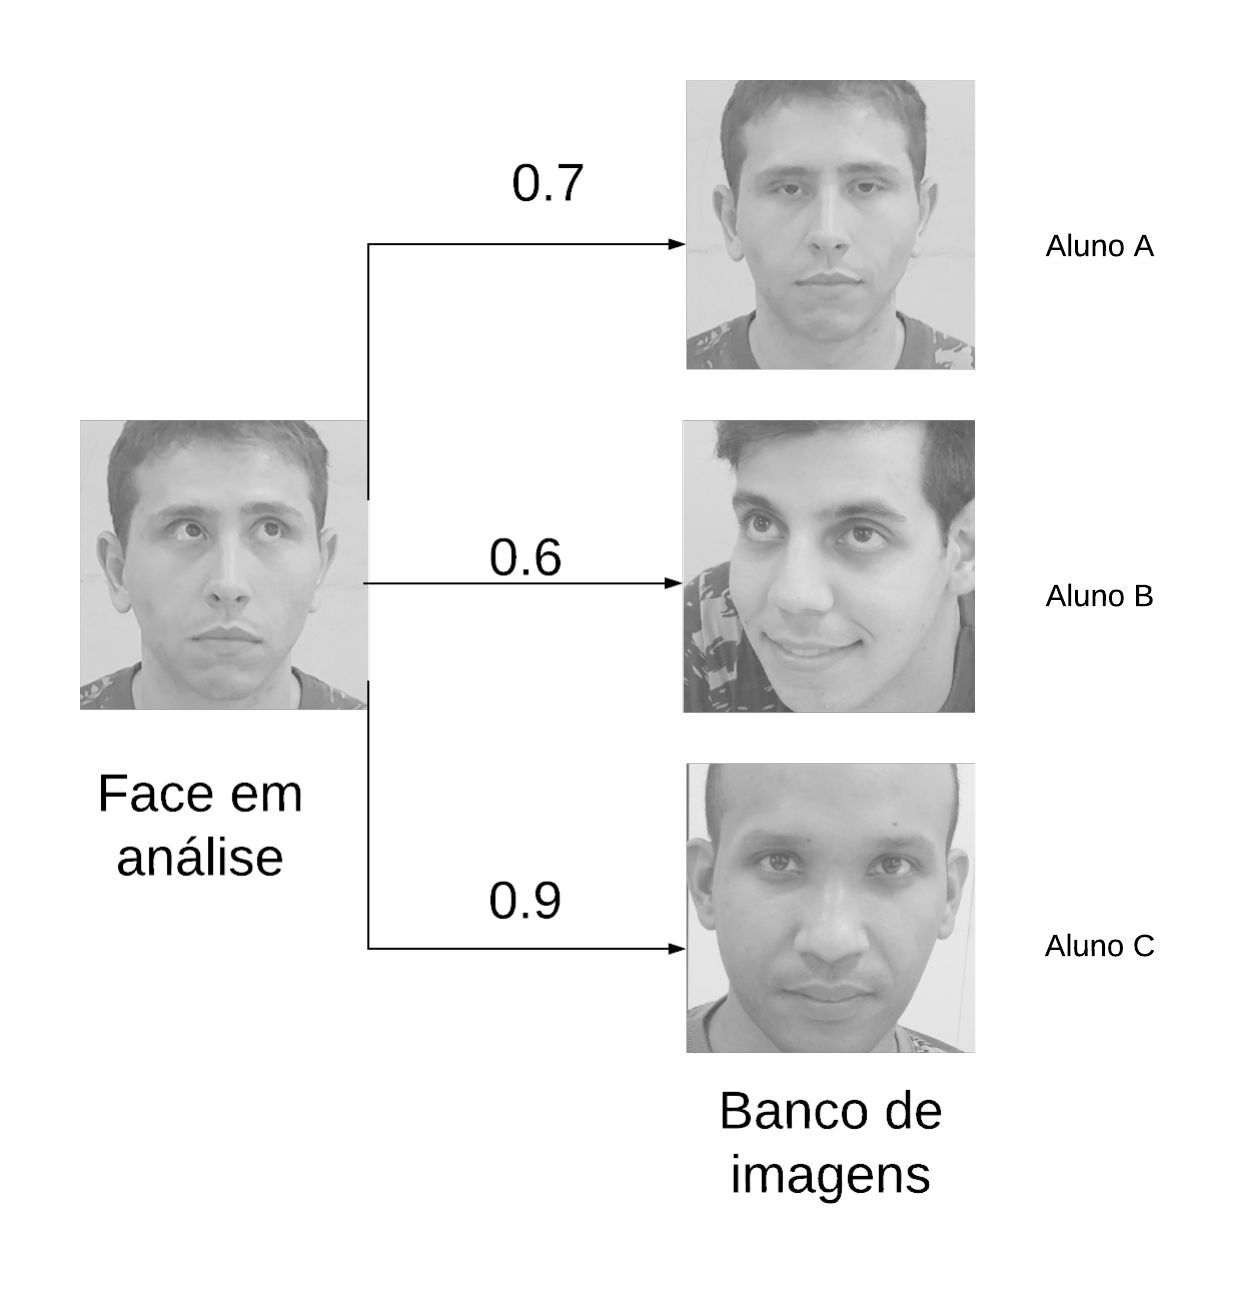
\includegraphics[width=0.6\textwidth]{threa.png}   
	\caption{Exemplo de distância menor que o limite, gerando classificação incorreta }
	\label{fig:figura53}
\end{figure}


A dificuldade na escolha desse parâmetro está no fato de quando é melhor classificar a face como desconhecida ao invés de tentar forçar uma classificação com distância maior, e que pode ser errada. Ao utilizar um valor elevado, pode-se forçar classificações erradas. Por outro lado, colocar valores baixos pode fazer com que se classifique uma face como desconhecida enquanto que ela poderia utilizar a classificação que lhe seria dada dentre o conjunto. Pensando no caso da figura \ref{fig:figura54}, caso fosse adotado um \textit{threshold} de 0.5, a análise concluiria que a face pertence a um elemento desconhecido. Por outro lado um \textit{threshold} de 0.7 seria suficiente para uma classificação correta.

\begin{figure}[!ht]
	\centering
	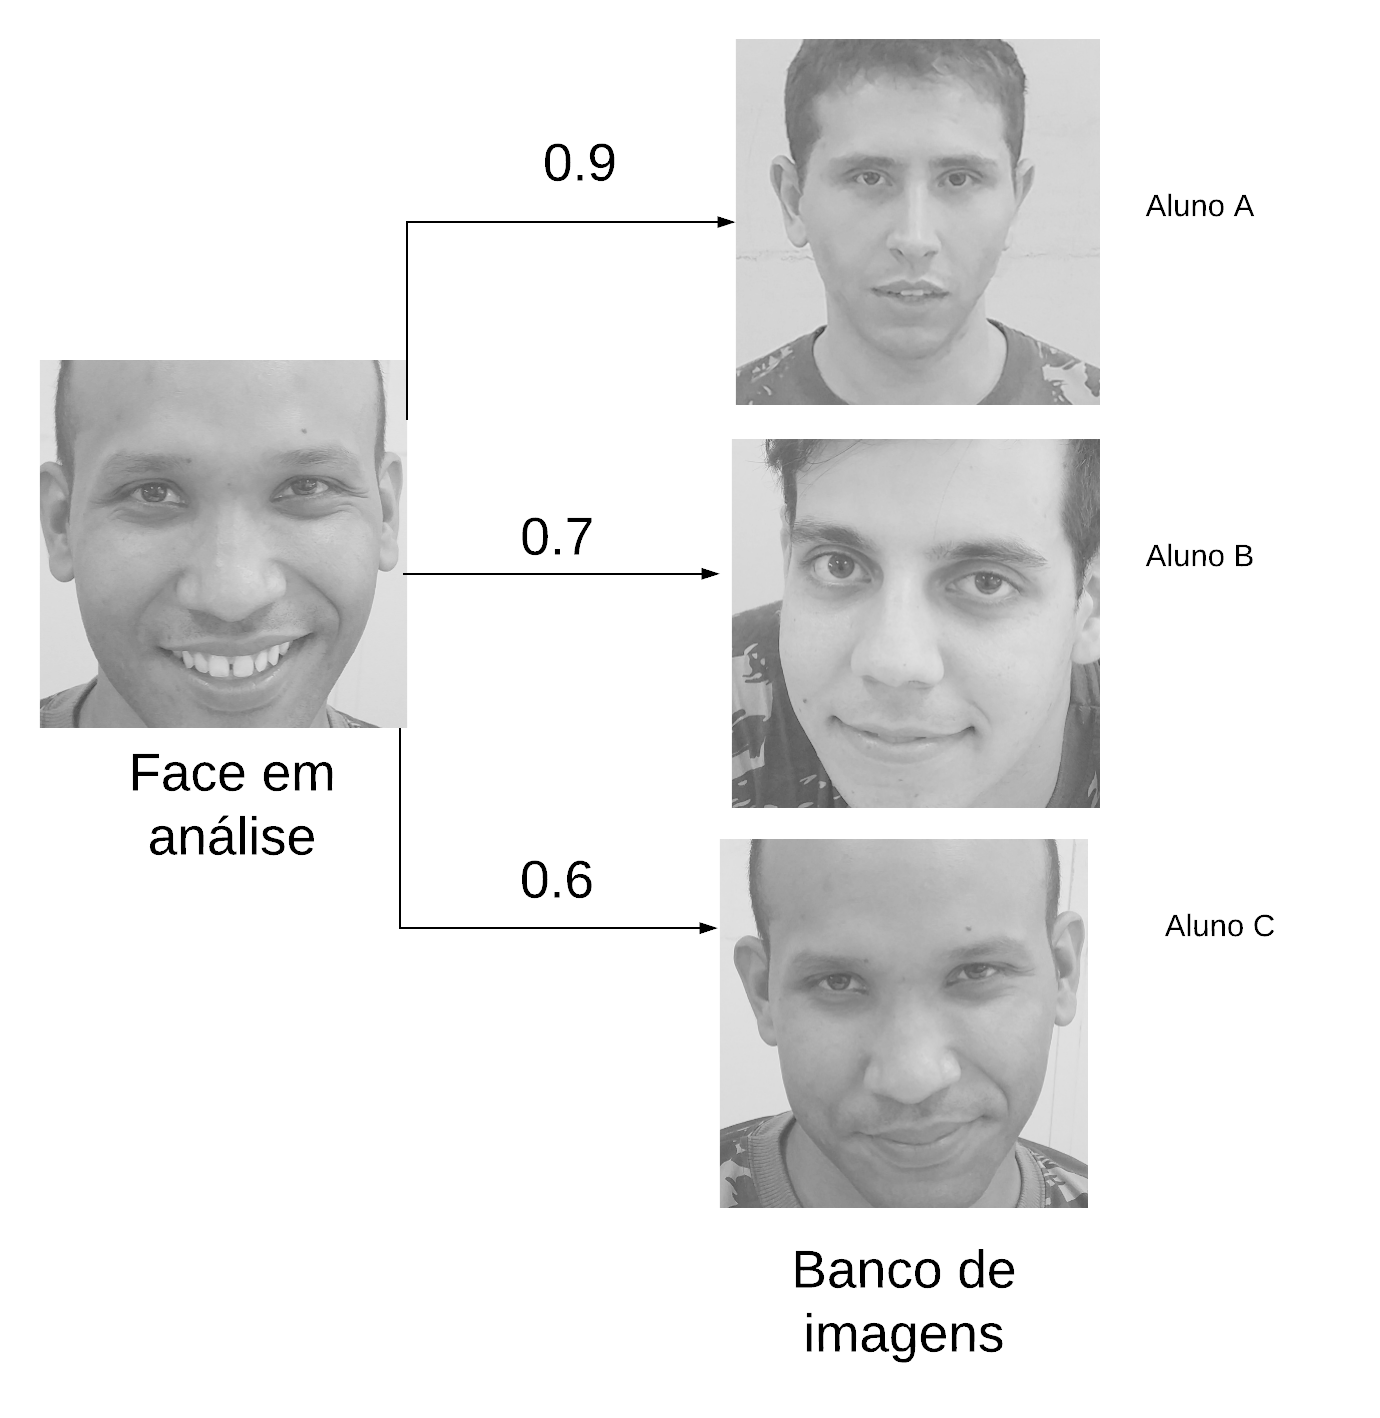
\includegraphics[width=0.6\textwidth]{threb.png}   
	\caption{Exemplo de distância maior que o limite, gerando classificação desconhecida }
	\label{fig:figura54}
\end{figure}

%Como saída do teste, obteve-se a Tabela \ref{tab:tabela1}, 
Feitas as considerações acima, realizou-se o procedimento similar ao descrito no início da subseção, isso é, utilizou-se o banco de imagens  disponibilizado pela Universidade de Yale \citep{yales}, contendo 165 imagens, dais quais 30 foram utilizadas para serem reconhecidas e as outras 135 para a geração do arquivo de treinamento. Ao gerar o arquivo de treinamento, utilizou-se como parâmetro os  encontrados anteriormente, \textit{radius = 1, neighbors = 8, grid\_x = 12, grid\_y = 12}. A Tabela \ref{tab:tabela2}, traz o valor de \textit{threshold}, a quantidade de faces detectadas com acerto, classificadas como desconhecidas e erradas. As quantidades estão em valores absolutos. Perceba que a classificação como desconhecida não é considerada como um erro, nem como um acerto. Em cada linha da tabela, a soma de acerto, desconhecida e erro totaliza 30, que é o número de imagens testadas.

% ii. tabelas: usar \begin{sidewaystable} ... \end{sidewaystable}
%                    em vez de \begin{table} ... \end{table}

\begin{table}[ht]
\centering
\caption{Testes para determinação do \textit{threshold}.}
\vspace{0.5cm}
\begin{tabular}{cccc}
 
threshold & Acerto & Desconhecida & Erro \\
\hline
10	& 3	& 27	& 0   \\
15	& 3	& 27	& 0  \\
20	& 3	& 27	& 0  \\
25	& 6	& 24	& 0  \\
30	& 7	& 23	& 0  \\
35	& 8	& 22	& 0  \\  
40	& 13	& 17	& 0  \\
45	& 17	& 13	& 0  \\
50	& 18	& 12	& 0  \\
55	& 18	& 12	& 0  \\
60	& 18	& 12	& 0  \\
65	& 18	& 11	& 1  \\
70	& 18	& 11	& 1  \\  
75	& 19	& 10	& 1  \\
80	& 19	& 9	& 2  \\
85	& 20	& 7	& 3  \\
90	& 20	& 5	& 5  \\
95	& 20	& 4	& 6  \\
100	& 20	& 3	& 7  \\
110	& 20	& 2	& 8  \\
130	& 21	& 0	& 9  \\


\end{tabular}
\label{tab:tabela2}
\end{table}

A Tabela \ref{tab:tabela2} corrobora aquilo que foi explicado nos parágrafos anteriores, a medida que se aumenta o valor do \textit{threshold}, o algoritmo é forçado a escolher a opção mais próxima daquela face. Com isso, a partir do valor 85, o que ocorre é a diminuição da quantidade de faces desconhecidas, mas um aumento do reconhecimento incorreto. Apenas no \textit{threshold = 130} é que todas faces são reconhecidas, como uma face conhecida. É nesse valor que se atinge o índice de acerto mencionado na Tabela \ref{tab:tabela1}, isso é, 70\% de acerto e nenhuma imagem classificada como desconhecida.

Na escolha do \textit{threshold}, o que deseja-se é maximilizar a taxa de acerto com uma mínima taxa de desconhecido. Da análise da Tabela \ref{tab:tabela2} verifica-se que a máxima quantidade de acertos combinada com a menor taxa de desconhecidos ocorreu com o  \textit{threshold} igual a 50; 55 e 60. Isso significa que do conjunto de imagens analisadas, nenhuma obteve uma distância no intervalo entre 50 e 60. Assim o desempenho dos 3 valores foi igual. Optou-se por utilizar o valor 50, por ser o menor valor do conjunto. Nesse caso, distâncias maiores que 50, levariam a uma classificação como desconhecida, evitando-se assim o erro. Assim, o \textit{threshold = 50}, dentre as imagens classificadas como conhecidas, obteve um índice de acerto de 100\%, além disso do conjunto de imagens 40\% foi classificado como desconhecido. Pensando em uma sala de aula, o professor teria a opção de enviar uma nova foto para ser reconhecida, em adição a que já foi analisada , ou mesmo poderia fazer as alterações manualmente. Procedimentos no momento da fotografia ajudam a diminuir a taxa de desconhecidos, como exibir o rosto o mais similar do que foi cadastrado (imagens do treinamento). 

Ainda no artefato "criador\_de\_inteligencia", pertencente ao módulo \textit{servidor}, como entrada, o usuário digita o nome da turma, então busca-se as fotografias já convertidas na etapa anterior dessa turma, usa-se o método \textit{train} da biblioteca OpenCV correspondente ao algoritmo LBPH. Tem-se então o processo de treinamento, ao final tem-se o arquivo que concatena as informações referentes a todas as fotografias de todos os alunos de uma turma. A figura \ref{fig:figura55} sintetiza esses procedimentos através de um diagrama de atividades. Perceba que os parâmetros pré-definidos referem-se aos valores estabelecidos para o presente projeto.


\begin{figure}[!ht]
	\centering
	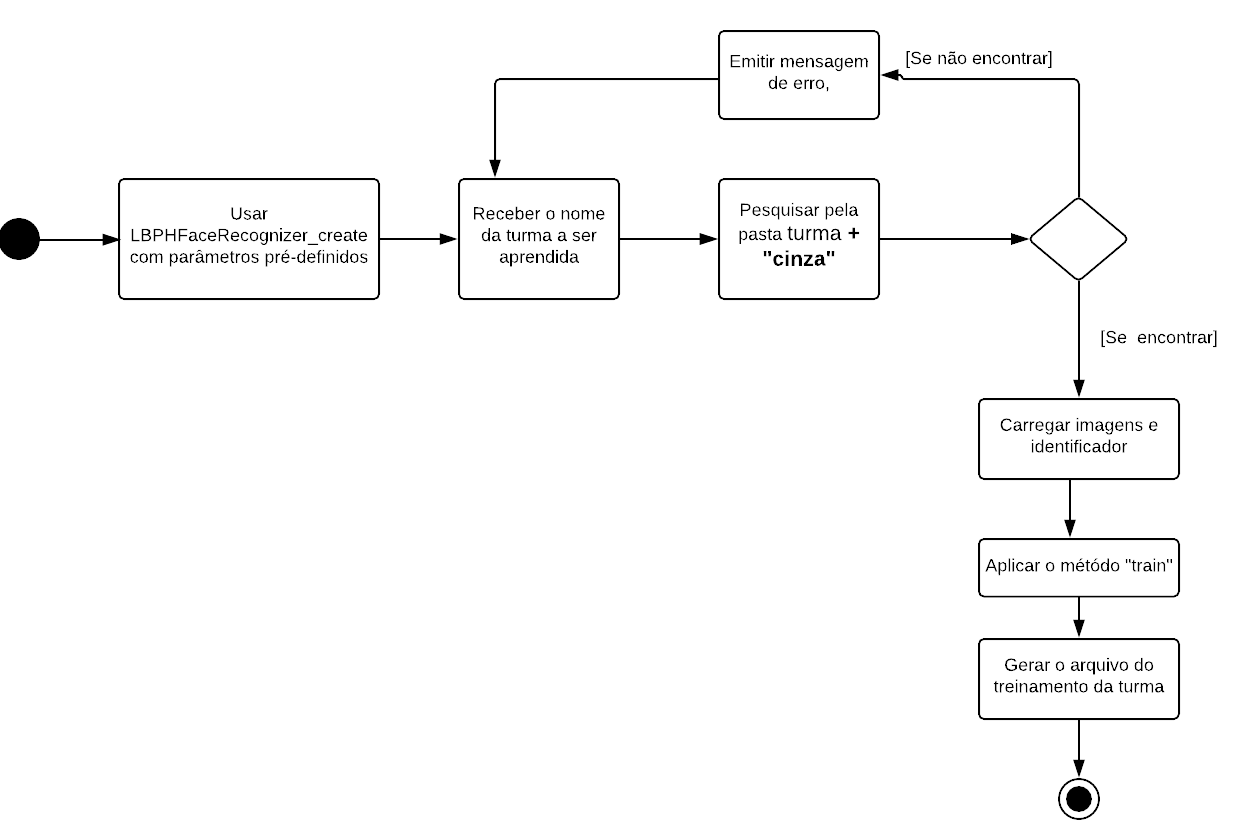
\includegraphics[width=1.0\textwidth]{diagramainteligencia.png}   
	\caption{Diagrama de atividades da fase treinamento}
	\label{fig:figura55}
\end{figure}

\section{O reconhecimento}
\noindent 
A etapa seguinte consiste em a partir de uma fotografia recebida da turma identificar quem nela encontra-se presente. Ela é realizada através do arquivo "reconhecimento\_final.py". 

Como mencionado no início do capítulo, inicialmente, ele procura por fotografias em uma pasta denominada "faltas". Quando detecta a presença de uma fotografia na pasta, inicia-se o processo. Do nome da foto, se extrai o nome da turma a qual ela pertence, a disciplina, o dia, mês e ano, o tempo de aula. A figura \ref{fig:figura56} mostra um exemplo com explicação dos campos, perceba que turma2 é o nome da turma e IA o nome da disciplina. A identificação da disciplina e do tempo de aula fazem-se necessárias, uma vez que uma disciplina pode durar  mais do que 1 tempo de aula. Assim, um aluno pode ter faltado ao 1º tempo, mas ter comparecido no 2º. 

\begin{figure}[!ht]
	\centering
	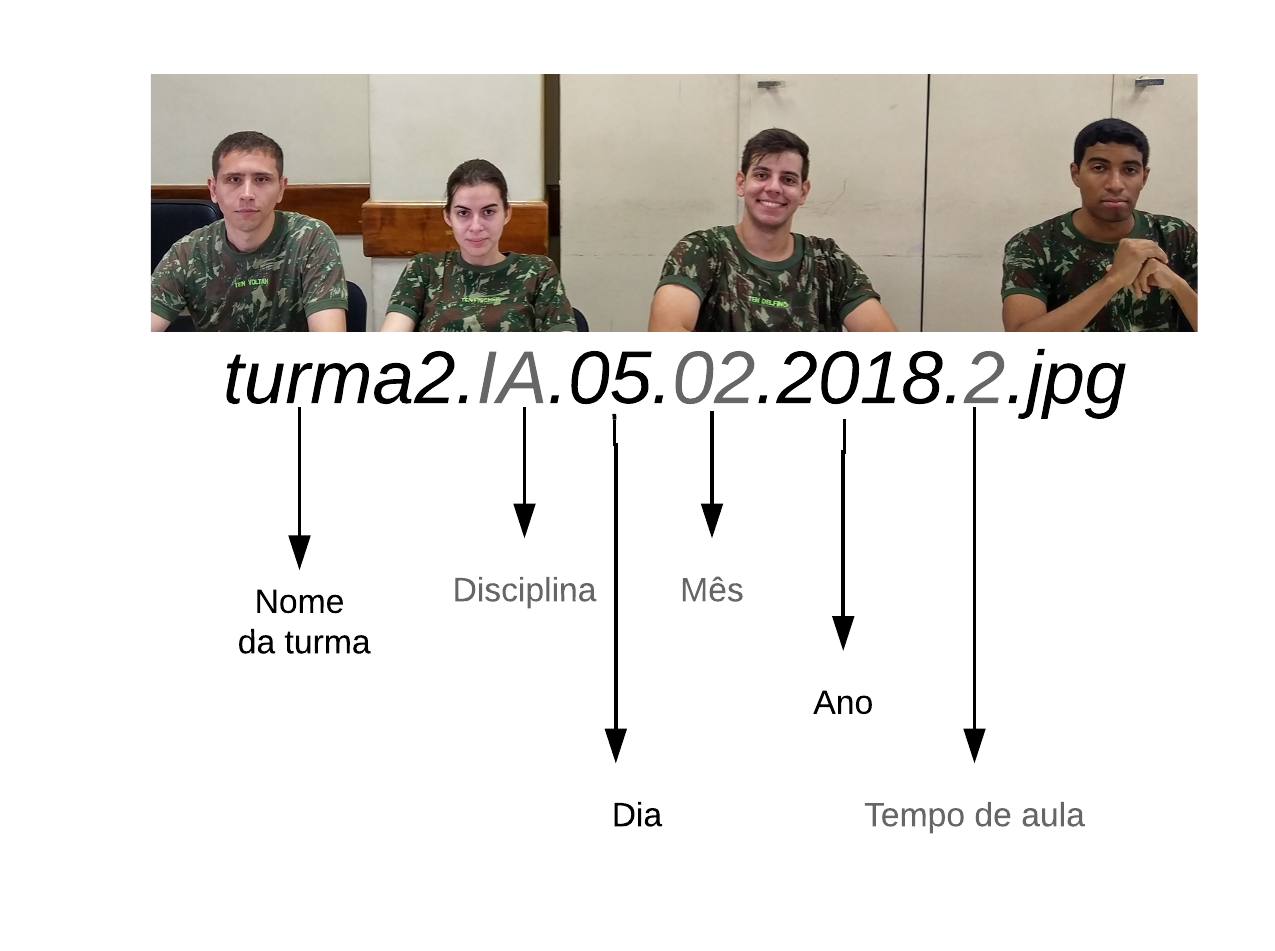
\includegraphics[width=0.7\textwidth]{nomenclaturaFotoTurma.png}   
	\caption{Exemplo de nome da foto}
	\label{fig:figura56}
\end{figure}

Ao encontrar uma imagem, ela é carregada, tratada, isso é, convertida para escala cinza, redimensionada e tem suas faces frontais detectadas. A partir do nome da turma, busca-se o arquivo que concatena as informações do banco de imagens daquela turma,  gerado na etapa treinamento. Tem-se aqui um ponto a ser destacado, o trabalho consiste em comparar características, usando o LBPH, daquela uma face com as faces previamente catalogadas para aquela turma. Como explicado, o algoritmo verifica a menor distância e depois compara com o\textit{threshold}. Cada uma das faces é reconhecida, ou no caso da menor distância ainda ser maior que o \textit{threshold}, ela é atribuída como desconhecida. O retorno do reconhecimento da face é o código do aluno. Aquele que teve sua face reconhecida tem sua presença computada. Em cada uma das faces detectadas, desenha-se o retângulo delimitador e a matrícula do aluno. Essas informações sobre composição de turma e o registro da presença serão realizadas utilizando-se o banco de dados, e serão abordadas com mais detalhes no capítulo 6, que tratará sobre o banco de dados.
%Em uma primeira fase desse projeto essas informações sobre composição de turma e presença estarão no próprio script em Python/saída. Na etapa futura, com a implementação do módulo BD, elas passarão a ser consultadas e salvas no próprio banco de dados.  

Após a imagem receber o retângulo com o nome do aluno, essas alterações são salvas e o arquivo migra para a pasta \textit{apuradas}. Ao nome da imagem, antes do formato, é feita a adição do caracter '.'  e o número daquela imagem, isso é, '.1' se for a primeira, '.2' se for a segunda e assim por diante. Por exemplo, caso a fotografia da figura \ref{fig:figura54} ao ser movida de pasta, verifique-se que foi a 5ª imagem apurada da turma2, na disciplina IA, no dia 05/02/2018 em seu 2º tempo de aula, então ao ser movido para a pasta apuradas, ela passaria a se chamar \textit{turma2.IA.05.02.2018.2.5.jpg}. 

A migração da imagem entre pastas garante que o laço \textit{while} não acabe tendo de verificar fotos que já foram apuradas. Além disso, a manutenção da imagem, em uma outra pasta, permite que caso algum aluno conteste  a falta, tenha-se um mecanismo alternativo para verificar essa informação. Nesse caso, a imagem da turma poderia ser utilizada, como mecanismo de verificação secundário. A figura \ref{fig:figura57} ilustra um diagrama de atividades para o "reconhecimento\_final.py". Nele, é possível verificar que o servidor procura pela fotografia na pasta faltas, quando encontra inicia seu processo de reconhecimento, e ao final transfere a fotografia apurada (com as faces identificadas por um retângulo branco com a matricula do aluno) para a pasta apuradas. Dessa forma ele está sempre verificando a pasta faltas.
   
\begin{figure}[!ht]
	\centering
	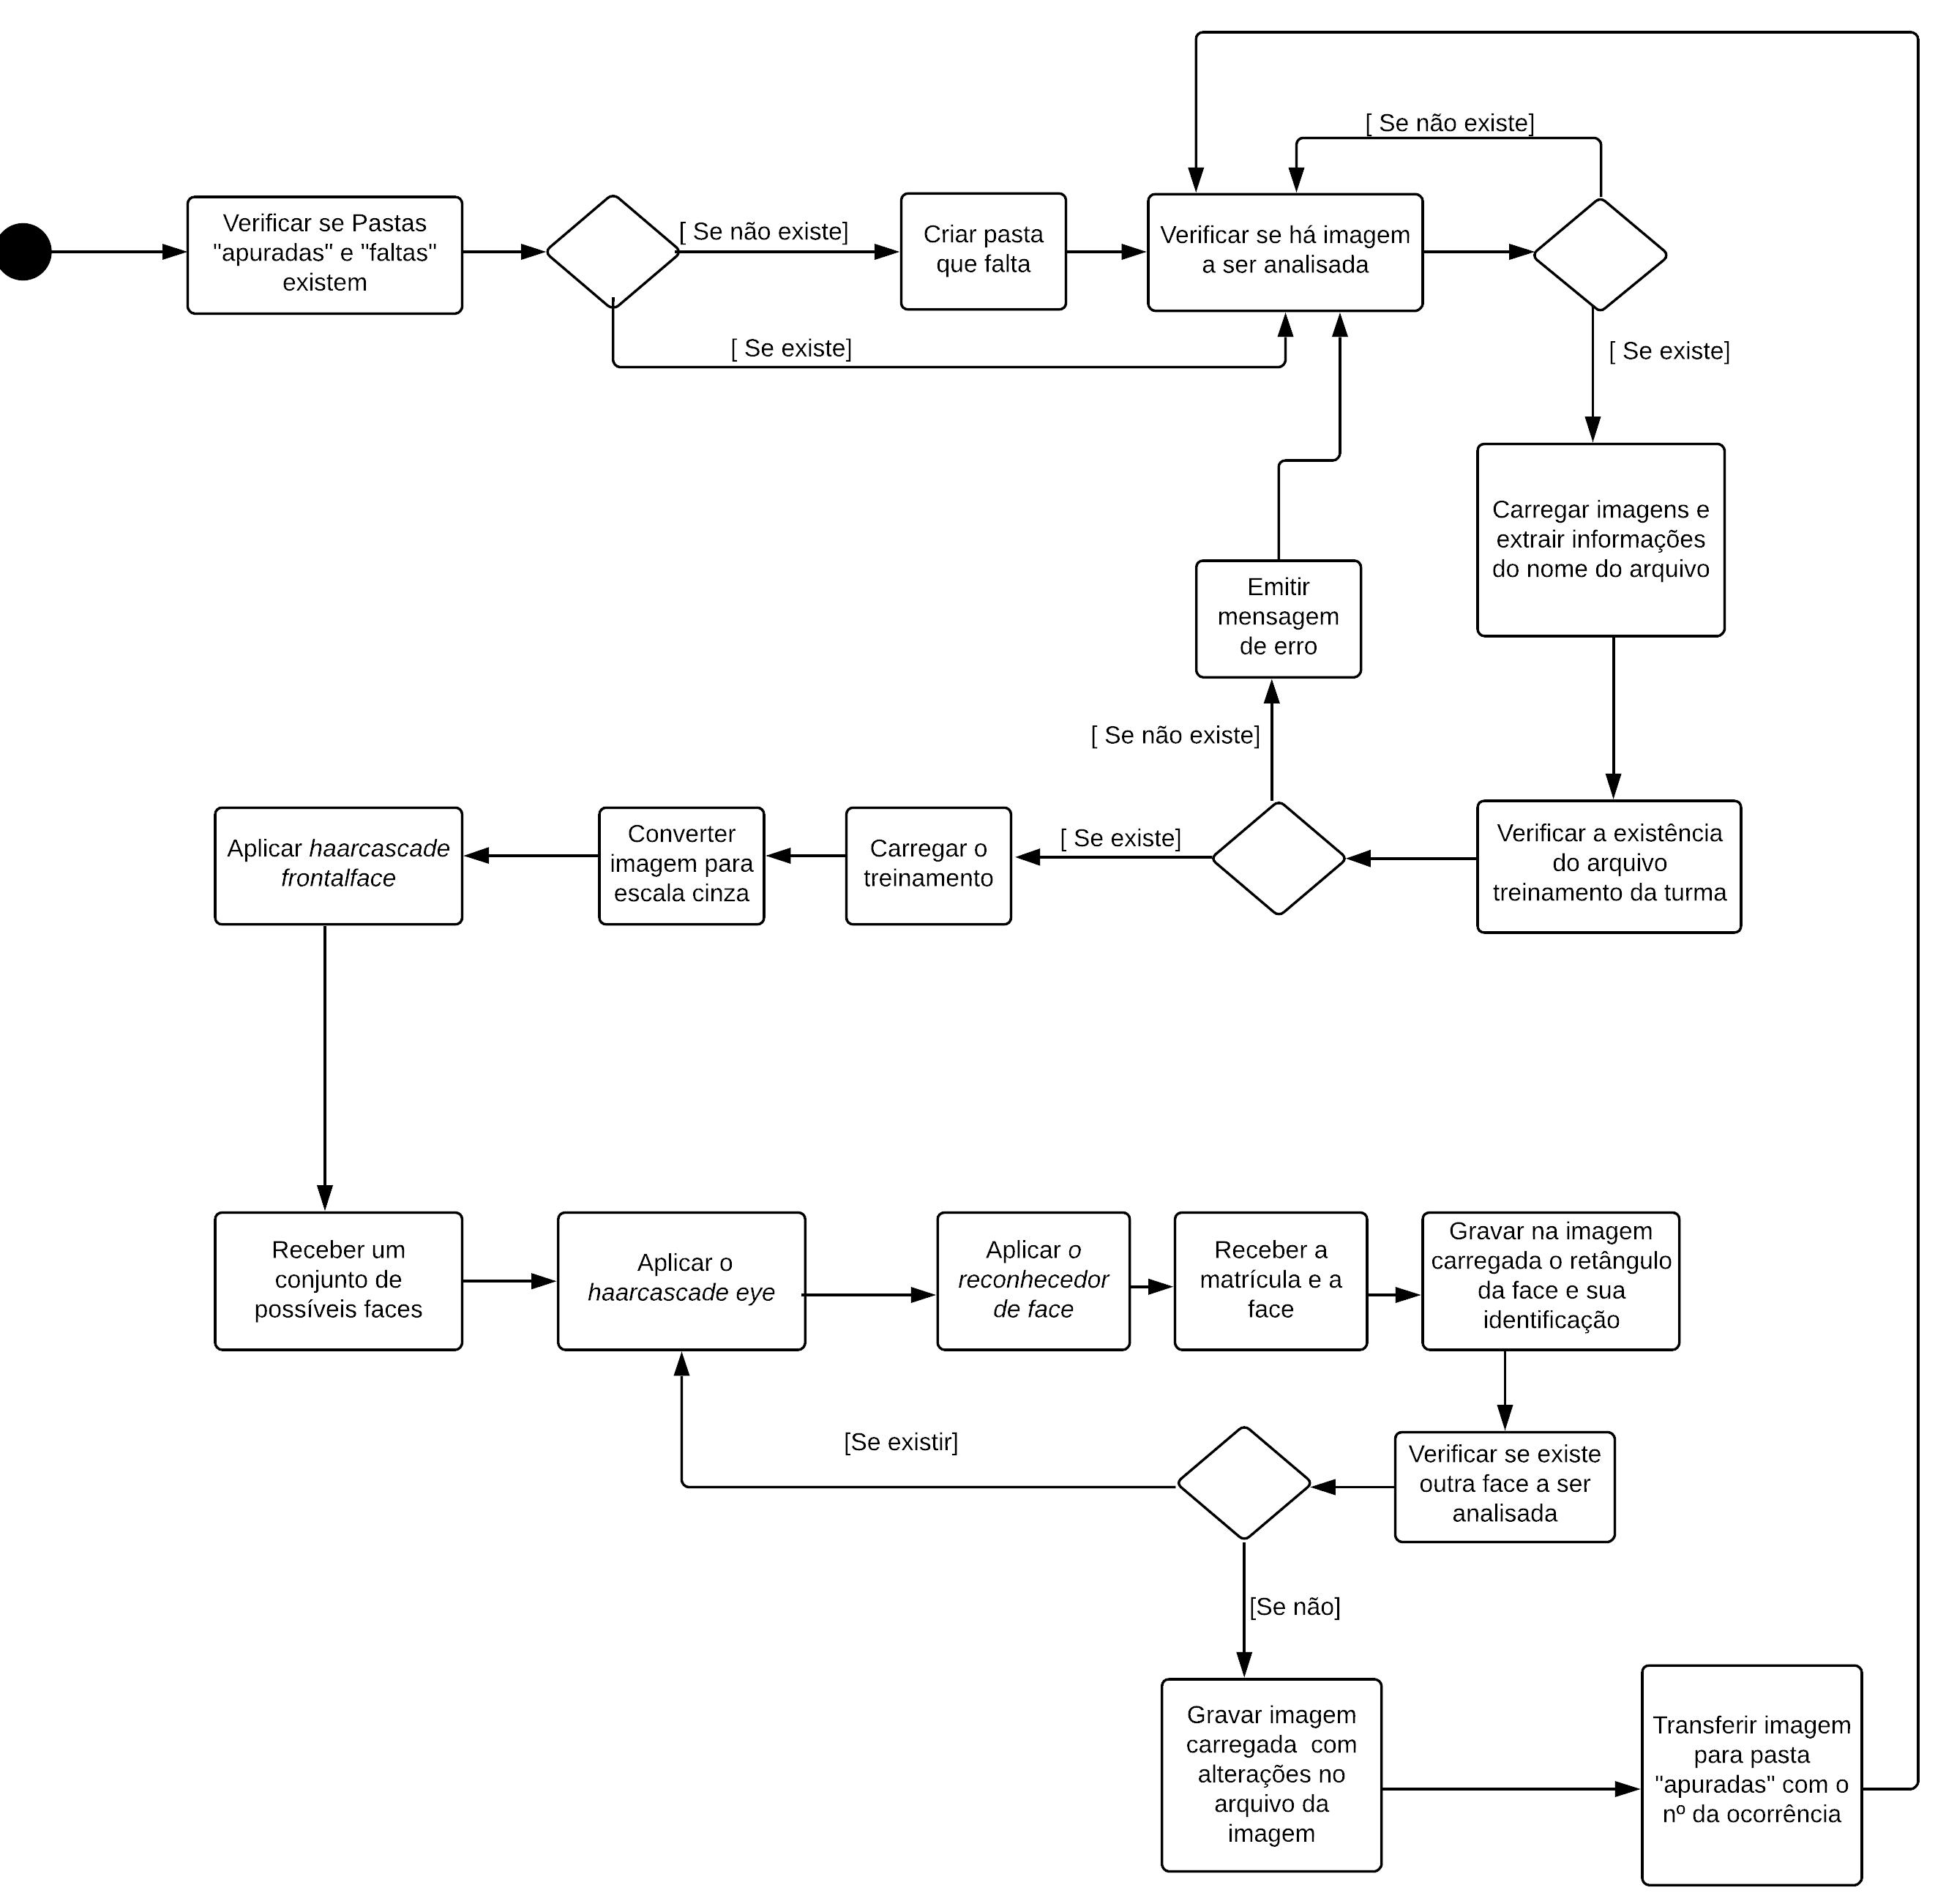
\includegraphics[width=1.0\textwidth]{diagramarec.png}   
	\caption{Diagrama de atividades da fase reconhecimento}
	\label{fig:figura57}
\end{figure}

A figura \ref{fig:figura58} ilustra em \textit{a)} a imagem de entrada do módulo Servidor, ou seja, a  recebida, e em \textit{b)} a imagem de saída, ou seja, a que será salva na pasta \textit{apuradas}. Comparando \textit{a)} e \textit{b)}, pode-se perceber que  adicionou-se o retângulo na face acompanhado da matrícula do aluno. Dessa forma atende-se o requisito funcional \textit{RF04 - Armazenar fotografia}.

\begin{figure}[!ht]
	\centering
	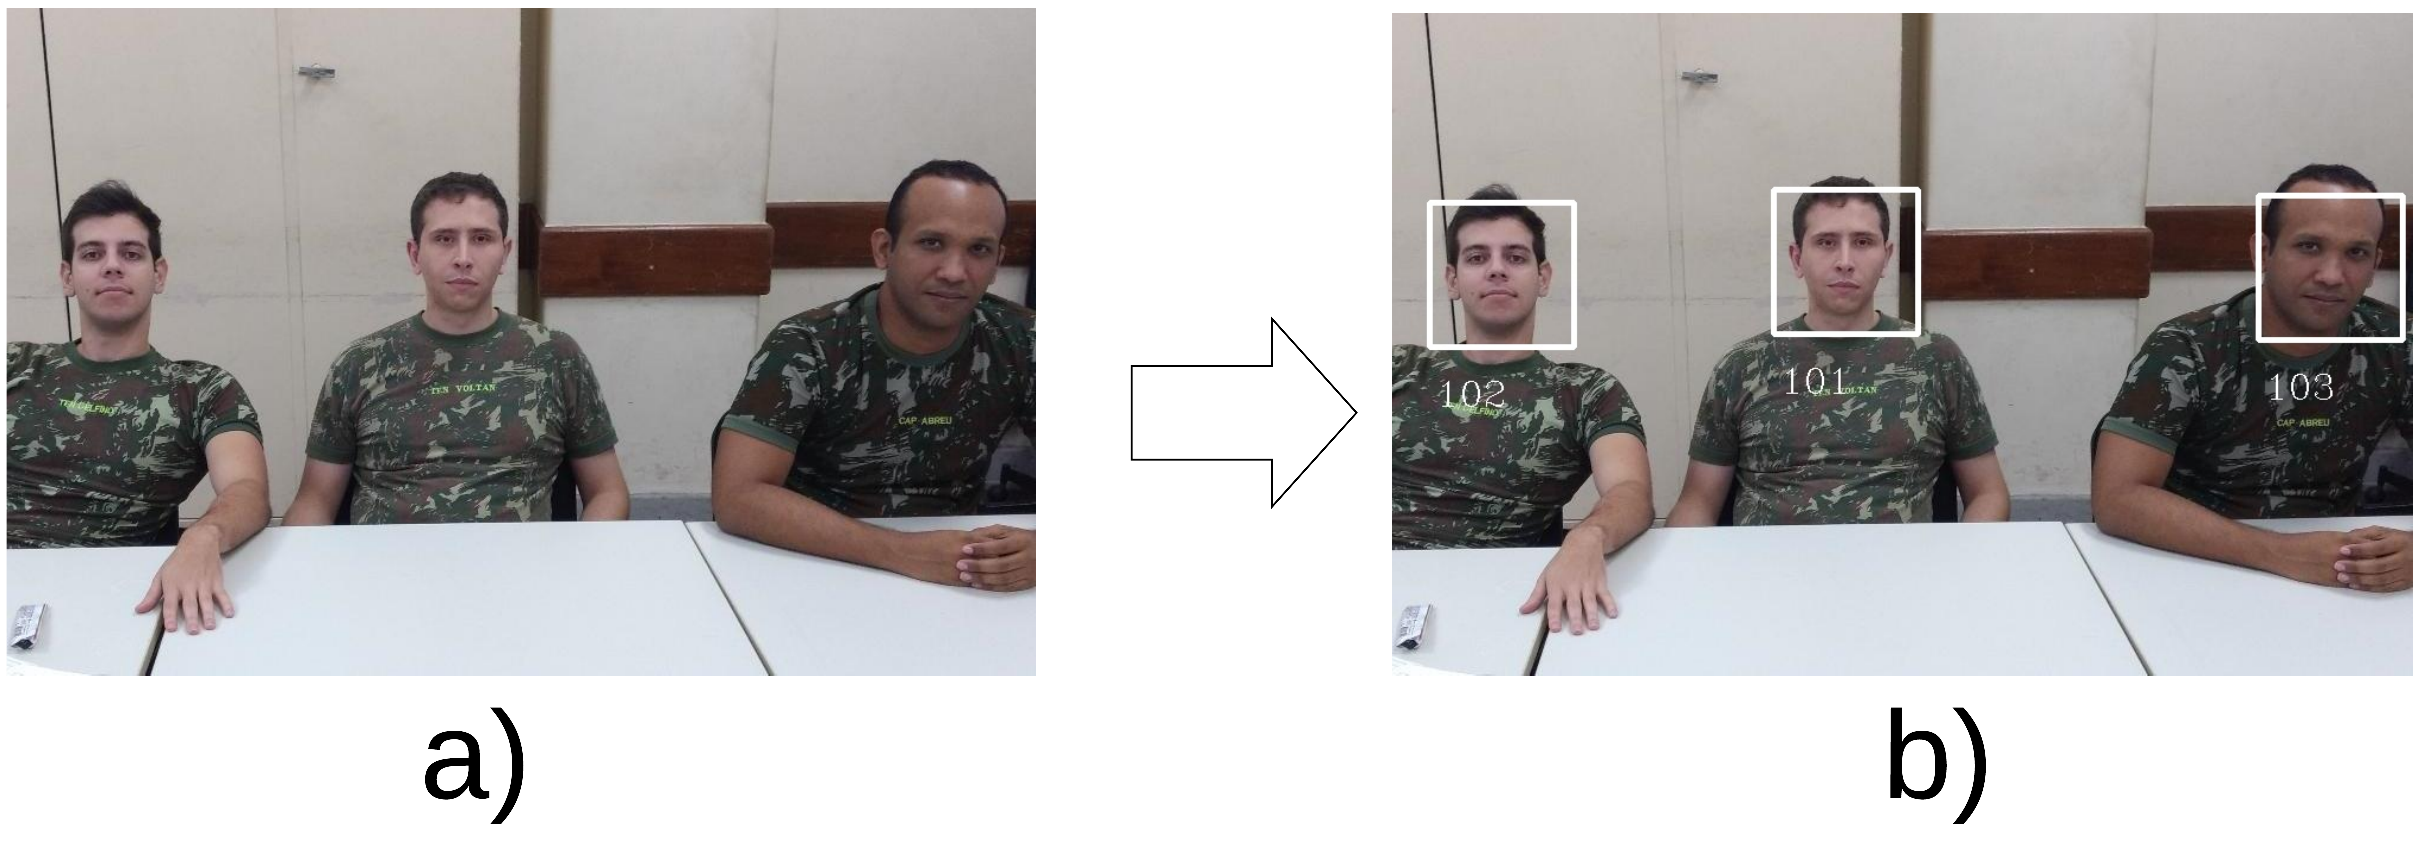
\includegraphics[width=1.0\textwidth]{antesdepoisbranco.png}   
	\caption{Entrada e saída do módulo Servidor}
	\label{fig:figura58}
\end{figure}

\chapter{Módulo Mobile}
\noindent
Este capítulo tem o objetivo de abordar o 2º módulo do projeto, o módulo \textit{mobile}. De maneira geral, ele é o responsável por retirar a fotografia da turma, captar os dados relativos ao código identificador, tempo de aula e, por fim, enviar toda a informação para o servidor e no servidor realizar o recebimento. O servidor conforme apresentado anteriormente, será responsável pela análise da foto. 
\section{Conceito Geral do módulo}
\noindent
Desenvolvido para plataforma Android, a aplicação deverá proporcionar ao usuário, professor, uma interface simples e intuitiva para a realização das tarefas propostas. O professor deve ser capaz de realizar a seleção de uma fotografia, já salva na galeria ou tirada no próprio momento, completar o registro de informações essenciais e realizar o posterior envio. O diagrama de atividades pode ser visto na figura \ref{fig:figura80}
\begin{figure}[!ht]
	\centering
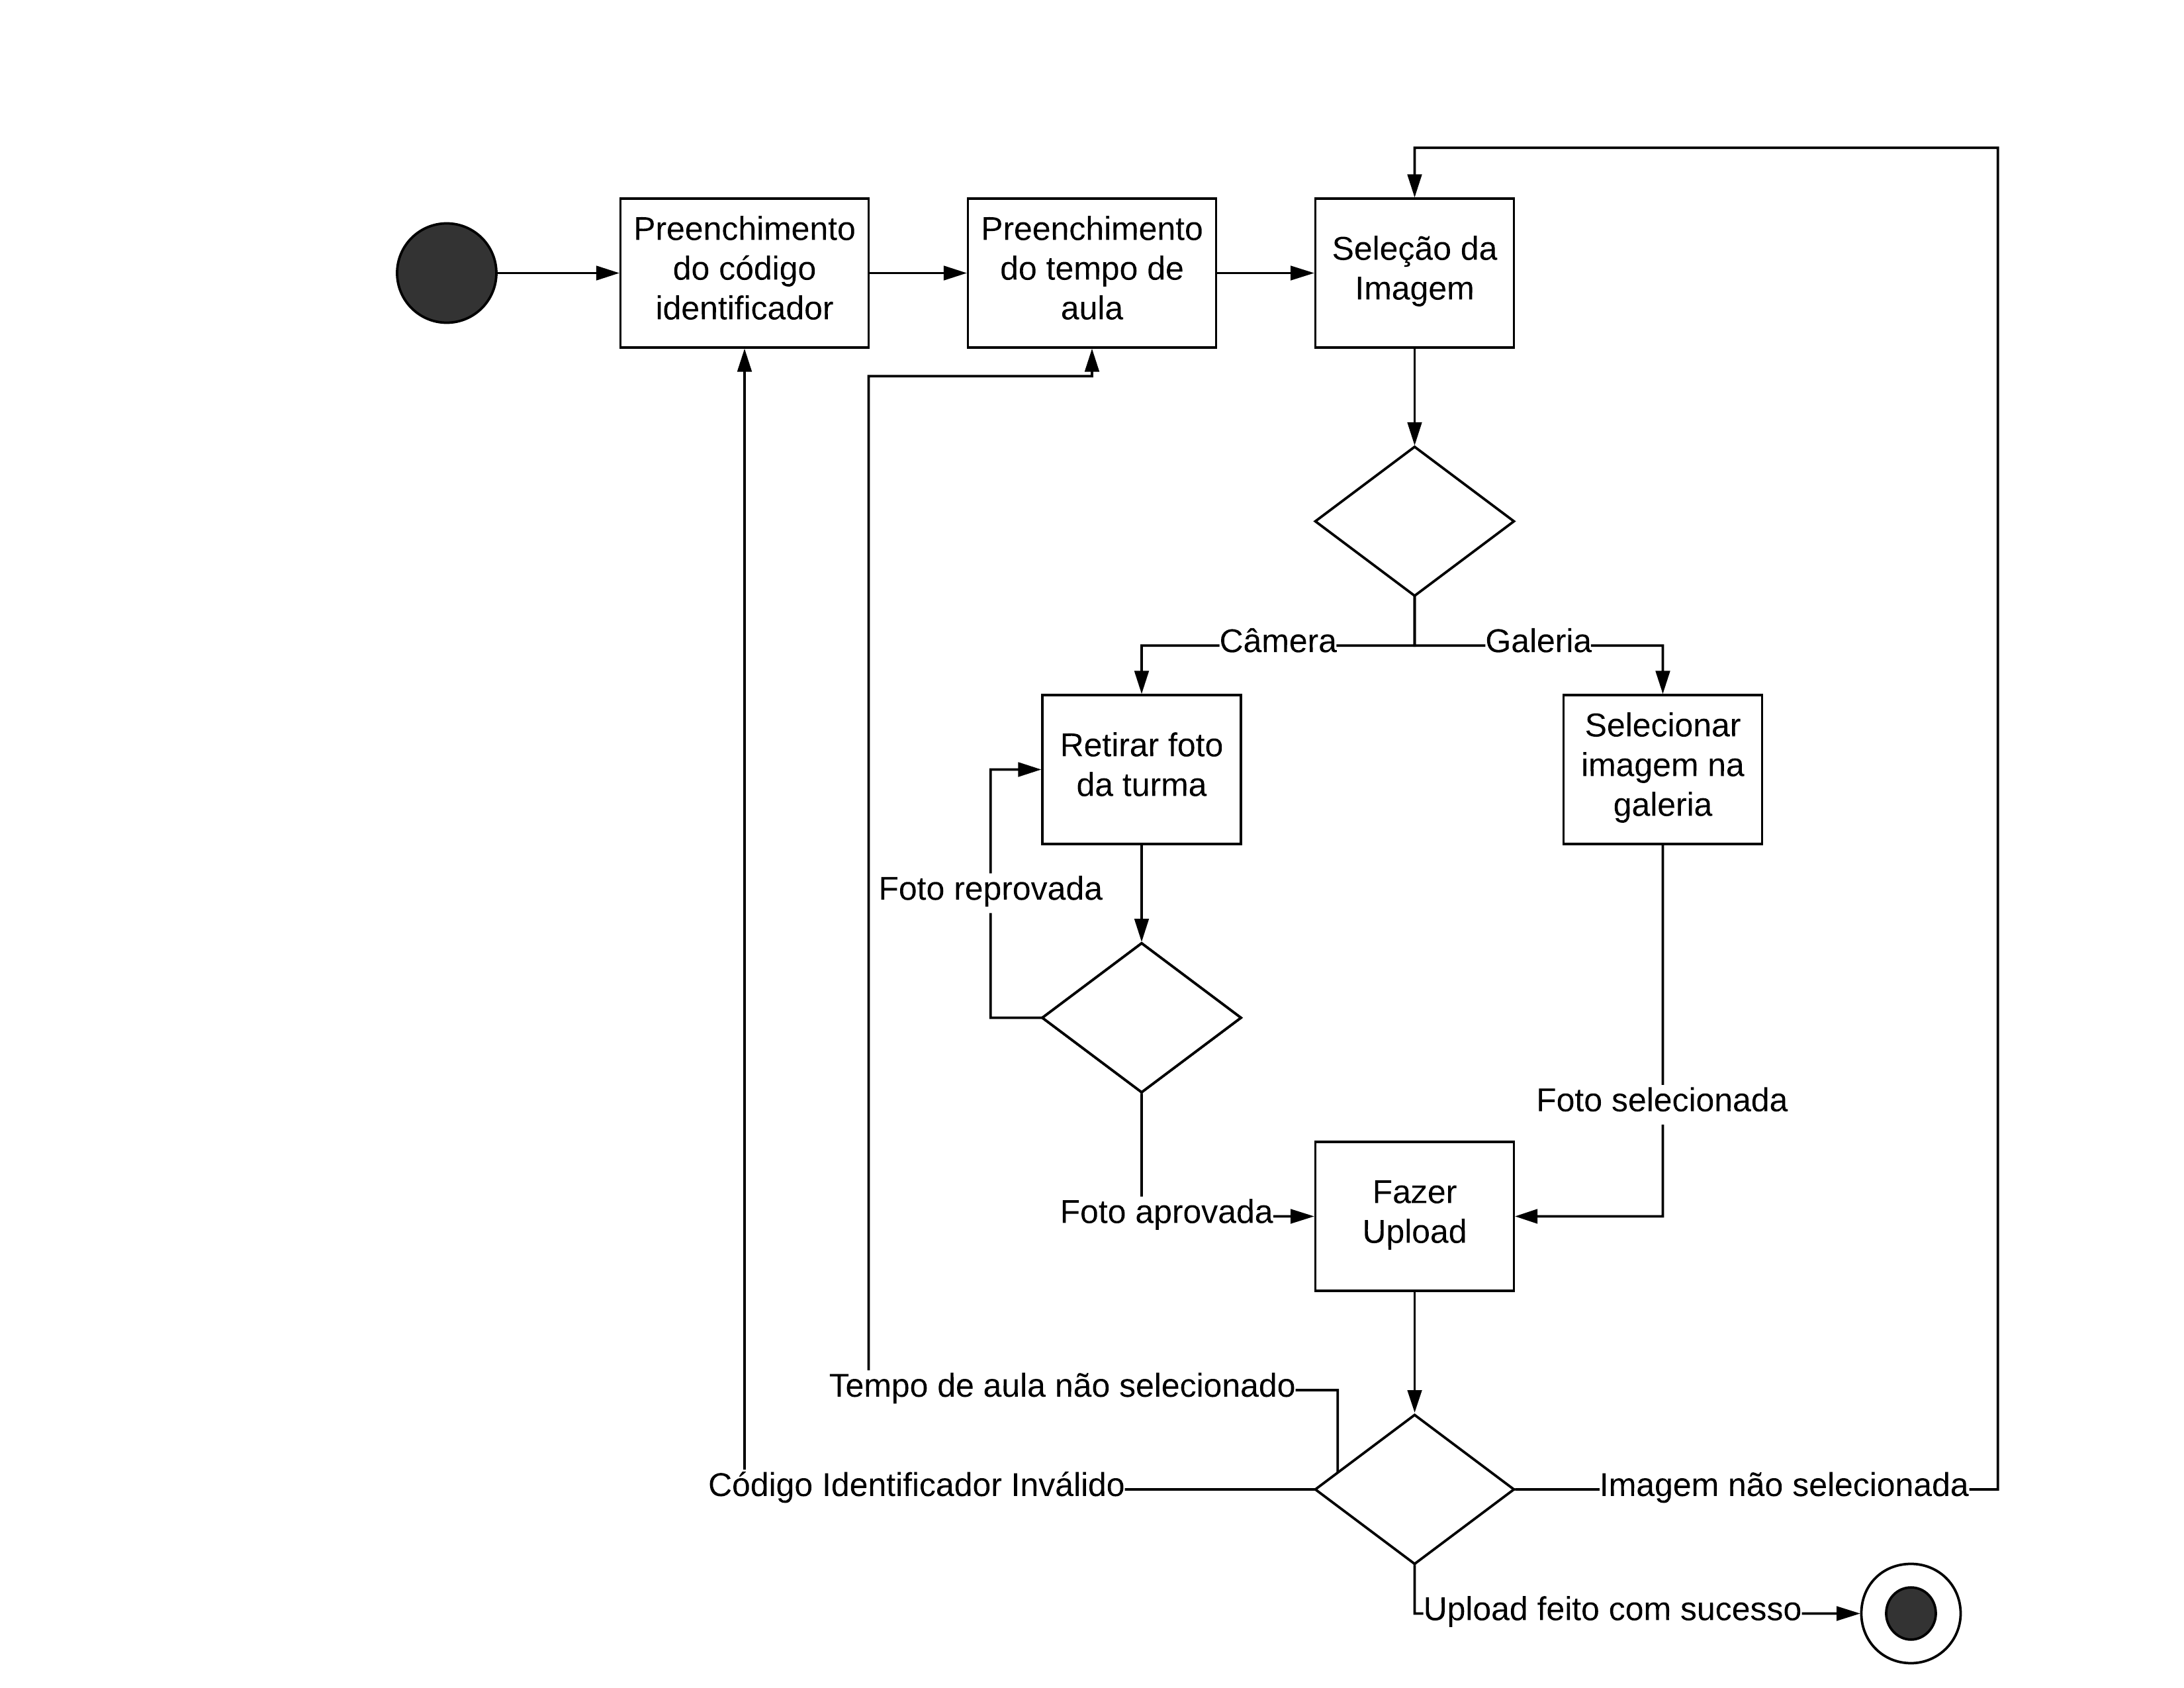
\includegraphics[width=1.0\textwidth]{diagrama_atividades.png}
	\caption{Diagrama de atividades}
	\label{fig:figura80}
\end{figure}

\section{Plataforma Android}
Android é uma plataforma móvel baseada em Linux, cujo desenvolvimento propunha já desde os primórdios um desenvolvimento sob padrão aberto, ou seja, um padrão que está disponível para o público \citep{Android1}. O projeto foi desenvolvido pelo consórcio de empresas de tecnologias Open Handset Alliance, contendo gigantes do mercado como Google, Sony, Samsung e outras operadoras de telefonia e fabricantes de dispositivos \citep{Android2}.  A pilha de software do Android pode ser vista em detalhes na figura \ref{fig:figura58b}, que mostra a maioria dos componentes da plataforma Android \citep{Android1}.

\begin{figure}[!ht]
	\centering
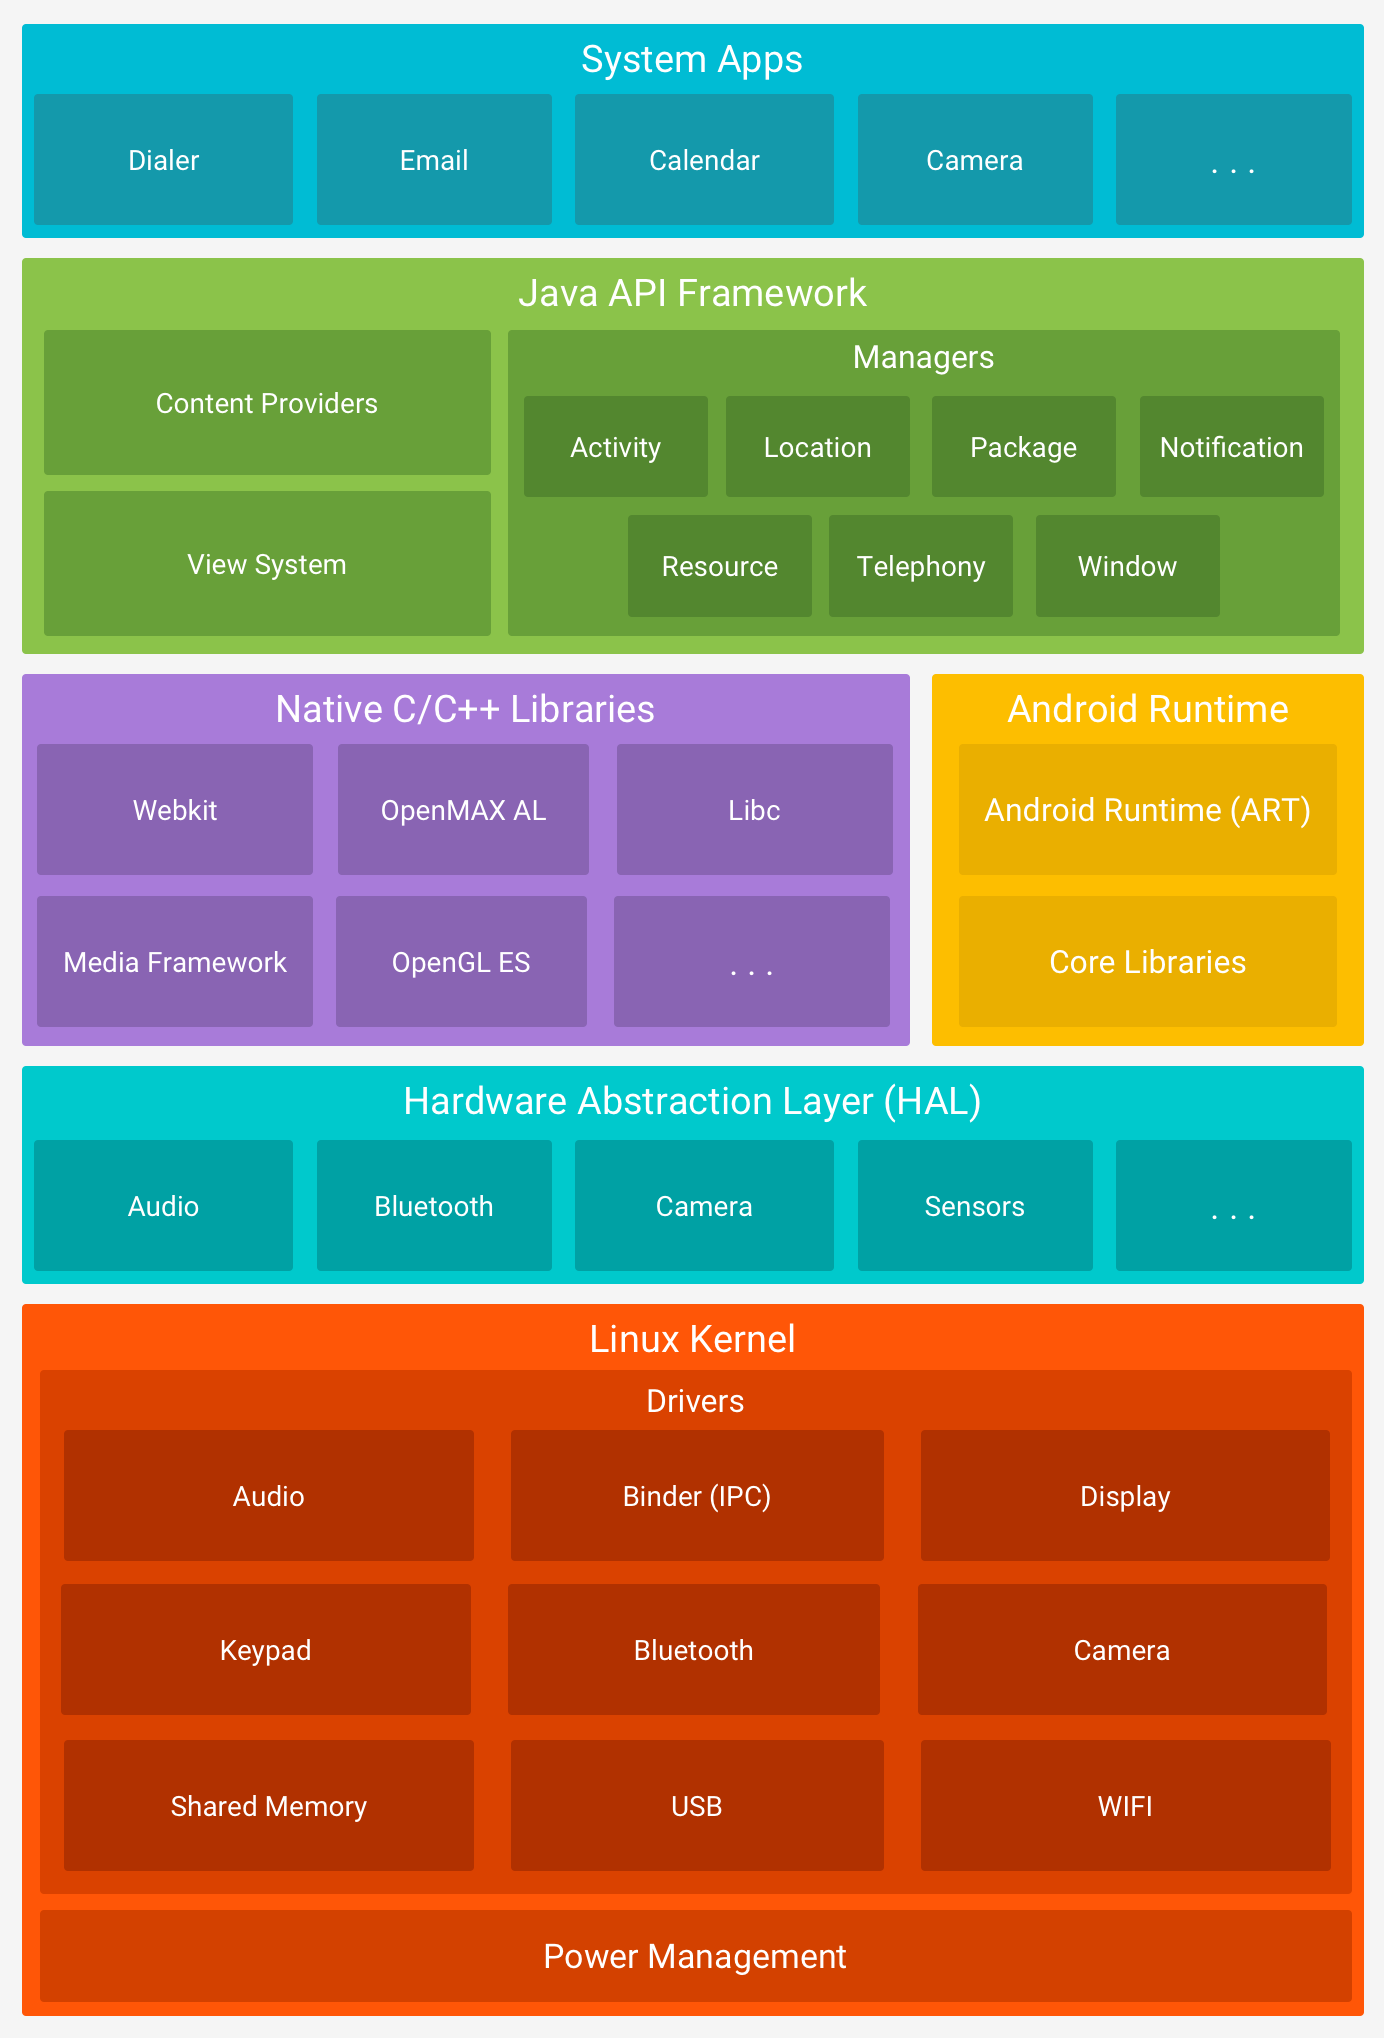
\includegraphics[width=0.6\textwidth]{arquitetura_android.png}   
	\caption{Pilha de software do Android v. abril 2018}\citep{Android1}
	\label{fig:figura58b}
\end{figure}



A equipe de desenvolvedores lideradas por Andy Rubinera criou no android a capacidade de acessar informações por meio de poucos toques extremamente intuitivos. Uma das grandes vantagens é tornar o sistema acessível para o usuário casual, ou seja, utilizadores que não possuem grande conhecimento tecnológico. De forma fluida, portanto, a plataforma permite a utilização dos mais diversos aplicativos sem demandar um processo de reaprendizado custoso por parte do usuário, visto que as características do dispositivos presente nos aplicativos torna familiar a experiência mesmo se tratando de novos aplicativos \citep{Android3}.

A possibilidade de usar componentes já prontos intrínsecos ao sistema operacional, como a interface de controle da câmera fotográfica, diminui o custo de desenvolvimento para o software em questão ao se escolher a plataforma Android, além de aumentar de forma relevante a qualidade do produto desenvolvido, já que os componentes reutilizados dentro da aplicação já foram exaustivamente testados antes de serem homologados e disponibilizados para uso. A utilização da câmera fotográfica através da aplicação pode ser vista na figura \ref{fig:figura59}.

Todos esses fatores fizeram com que a plataforma Android dominasse o mercado de maneira avassaladora. Segundo pesquisa liderada pela corporação IDC, International Data Corporation, no primeiro quarto de ano de 2017, a plataforma estava presente em 85\% dos aparelhos mobile ao redor do mundo, justificando o rótulo de plataforma mais popular do mundo, presente até mesmo no site oficial Android \citep{Android4} \citep{Android5}. No Brasil, a hegemonia é ainda mais significante, segundo dados da empresa Kantar, tendo alcançado 93\% do mercado nacional em março de 2018 \citep{Android6}.

Esses dados corroboram a escolha da plataforma para construção do aplicativo, que busca ser o mais acessível possível.


\subsection{Ambiente de desenvolvimento}
Buscando tornar o aplicativo o mais acessível possível, este foi desenvolvido tendo como base a API 15: Android 4.0.3 (\textit{IceCreamSandwich}), sendo compatível com quase a totalidade de aplicativos existentes, segundo estatísticas do próprio Android Studio.
%\begin{figure}[!ht]
%	\centering
%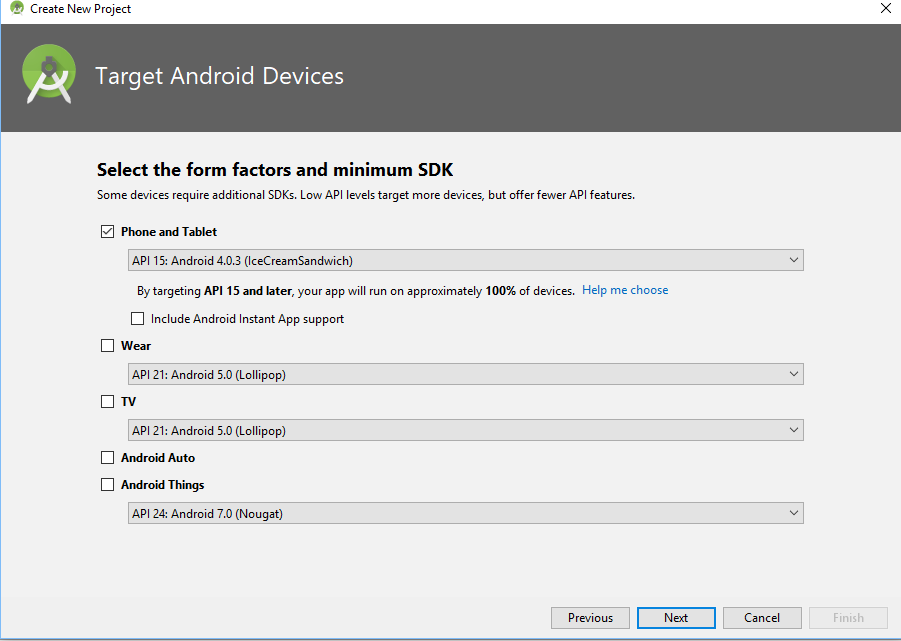
\includegraphics[width=1.0\textwidth]{target_devices.png}   
%	\caption{Dispositivos compatíveis}
%	\label{fig:figura60}
%\end{figure}

Utilizou-se a versão estável mais atual do Android Studio, visando tornar o código compatível com os recursos mais recentes oferecidos por esse ambiente de desenvolvimento. A figura \ref{fig:figura61} contém as informações sobre a versão utilizada, contruída em 4 de Junho de 2018.
\begin{figure}[!ht]
	\centering
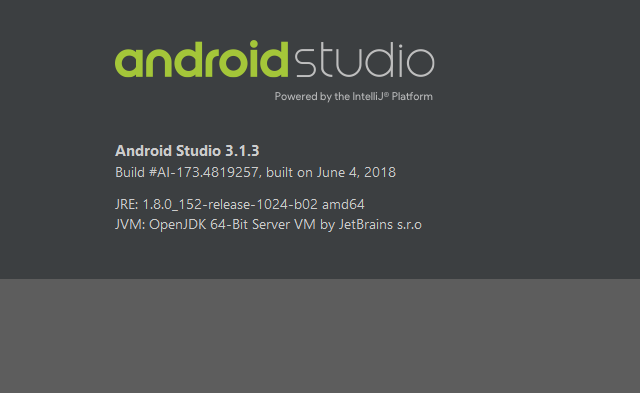
\includegraphics[width=0.55\textwidth]{versao_android.png}   
	\caption{Versão Android}
	\label{fig:figura61}
\end{figure}

\subsection{Linguagem de programação}
A linguagem de programação utilizada foi Java, utilizada pelo Android Software Development Kit, SDK. A utilização do SDK é a escolha recomendada oficialmente pela Google, visto que a Android Native Development Kit, NDK, só é aconselhável caso verdadeiramente se necessite ganhar maior desempenho, já que se rodaria a aplicação diretamente no processador \citep{Android7}. Esse ganho extra de desempenho, que aumentaria a complexidade do código, não é justificável visto que o processamento exigido durante toda a aplicação é extremamente reduzido. Além disso, ao utilizar o SDK se tem a garantia de portabilidade de dispositivo independentemente da arquitetura do processador, corroborando com a tentativa de tornar o aplicativo o mais acessível quanto possível \citep{Android8}.


\subsection{Dispositivos de teste}
Os dispositivos, ilustrados pelas figuras \ref{fig:figura62} e \ref{fig:figura63}, foram utilizados neste projeto para
a realização de testes da aplicação desenvolvida.

\begin{figure}[!ht]
	\centering
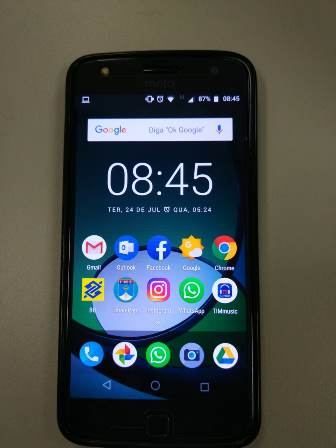
\includegraphics[width=0.25\textwidth]{img/moto_z_play.jpeg}   
	\caption{MOTO Z Play - Processador Snapdragon™ 625 Qualcomm® 3GB de RAM}
	\label{fig:figura62}
\end{figure}


\begin{figure}[!ht]
	\centering
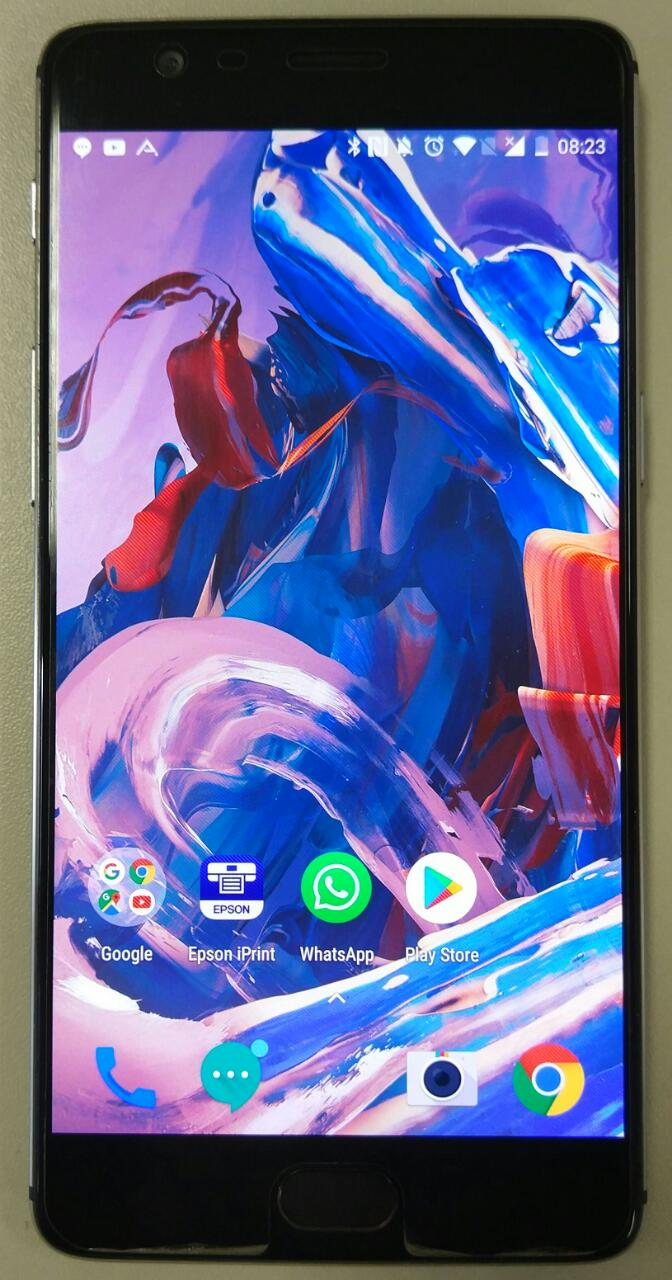
\includegraphics[width=0.15\textwidth]{img/Oneplus3.jpg}
	\caption{One Plus 3 - Processador Snapdragon™ 820 Qualcomm® 6GB de RAM}
	\label{fig:figura63}
\end{figure}

Nenhuma diferença de desempenho foi observada ao utilizar a aplicação nos diferentes dispositivos. Ambos aparelhos foram testados utilizando o Android 8.0.0. 

A única funcionalidade da aplicação verdadeiramente dependente de alguma característica do dispositivo é o acionamento da câmera, cuja utilização através da aplicação só pode ser executada caso o dispositivo possua câmera. Colocou-se uma verificação que libera o clique de acesso a câmera apenas para aqueles dispositivos que possuem o hardware. Devido a incapacidade de tirar fotos caso a câmera não exista, a verificação impede que o aplicativo gere um erro crítico. Ainda assim, contudo, é possível realizar envio completo das informações para retirada de faltas mesmo em um celular sem câmera, bastando utilizar uma imagem salva na galeria. A utilização da câmera através da aplicação pode ser revista na figura \ref{fig:figura59}, já mencionada anteriormente.

\begin{figure}[!ht]
	\centering
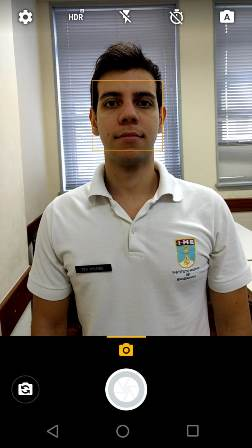
\includegraphics[width=0.2\textwidth]{img/camera_1.jpeg}   
	\caption{Utilização da câmera através da aplicação}
	\label{fig:figura59}
\end{figure}

\newpage
\section{A aplicação}
O objetivo da aplicação, conforme descrito no início do capítulo é garantir o preenchimento de informações necessárias para a retirada de faltas de maneira fluída e intuitiva. A figura \ref{fig:figura64} mostra a tela inicial da aplicação.


\begin{figure}[!ht]
	\centering
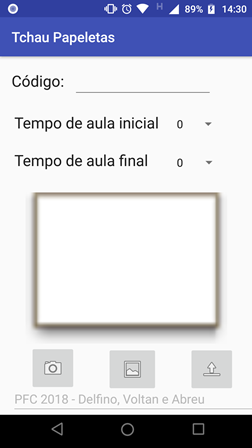
\includegraphics[width=0.3\textwidth]{Tela_Inicial_Aplicacao.png}   
	\caption{Tela inicial da aplicação}
	\label{fig:figura64}
\end{figure}

\subsection{Preenchimento do código identificador}
O preenchimento do código identificador, figura \ref{fig:figura65} ocorre ao clicar-se sobre o campo destinado para o mesmo, quando abrir-se-á o teclado e o professor poderá digitar a referência à turma e à matéria por ele ministrada. No exemplo a seguir, ilustradro na figura \ref{fig:figura66}, tem-se turma1 e disciplina Redes1, gerando o código identificador "turma1.Redes1". 

\begin{figure}[!ht]
	\centering
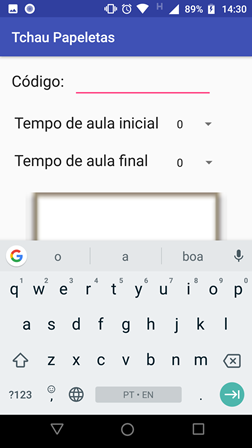
\includegraphics[width=0.3\textwidth]{Preenchimento_c_digo.png}   
	\caption{Teclado para digitação}
	\label{fig:figura65}
\end{figure}

\begin{figure}[!ht]
	\centering
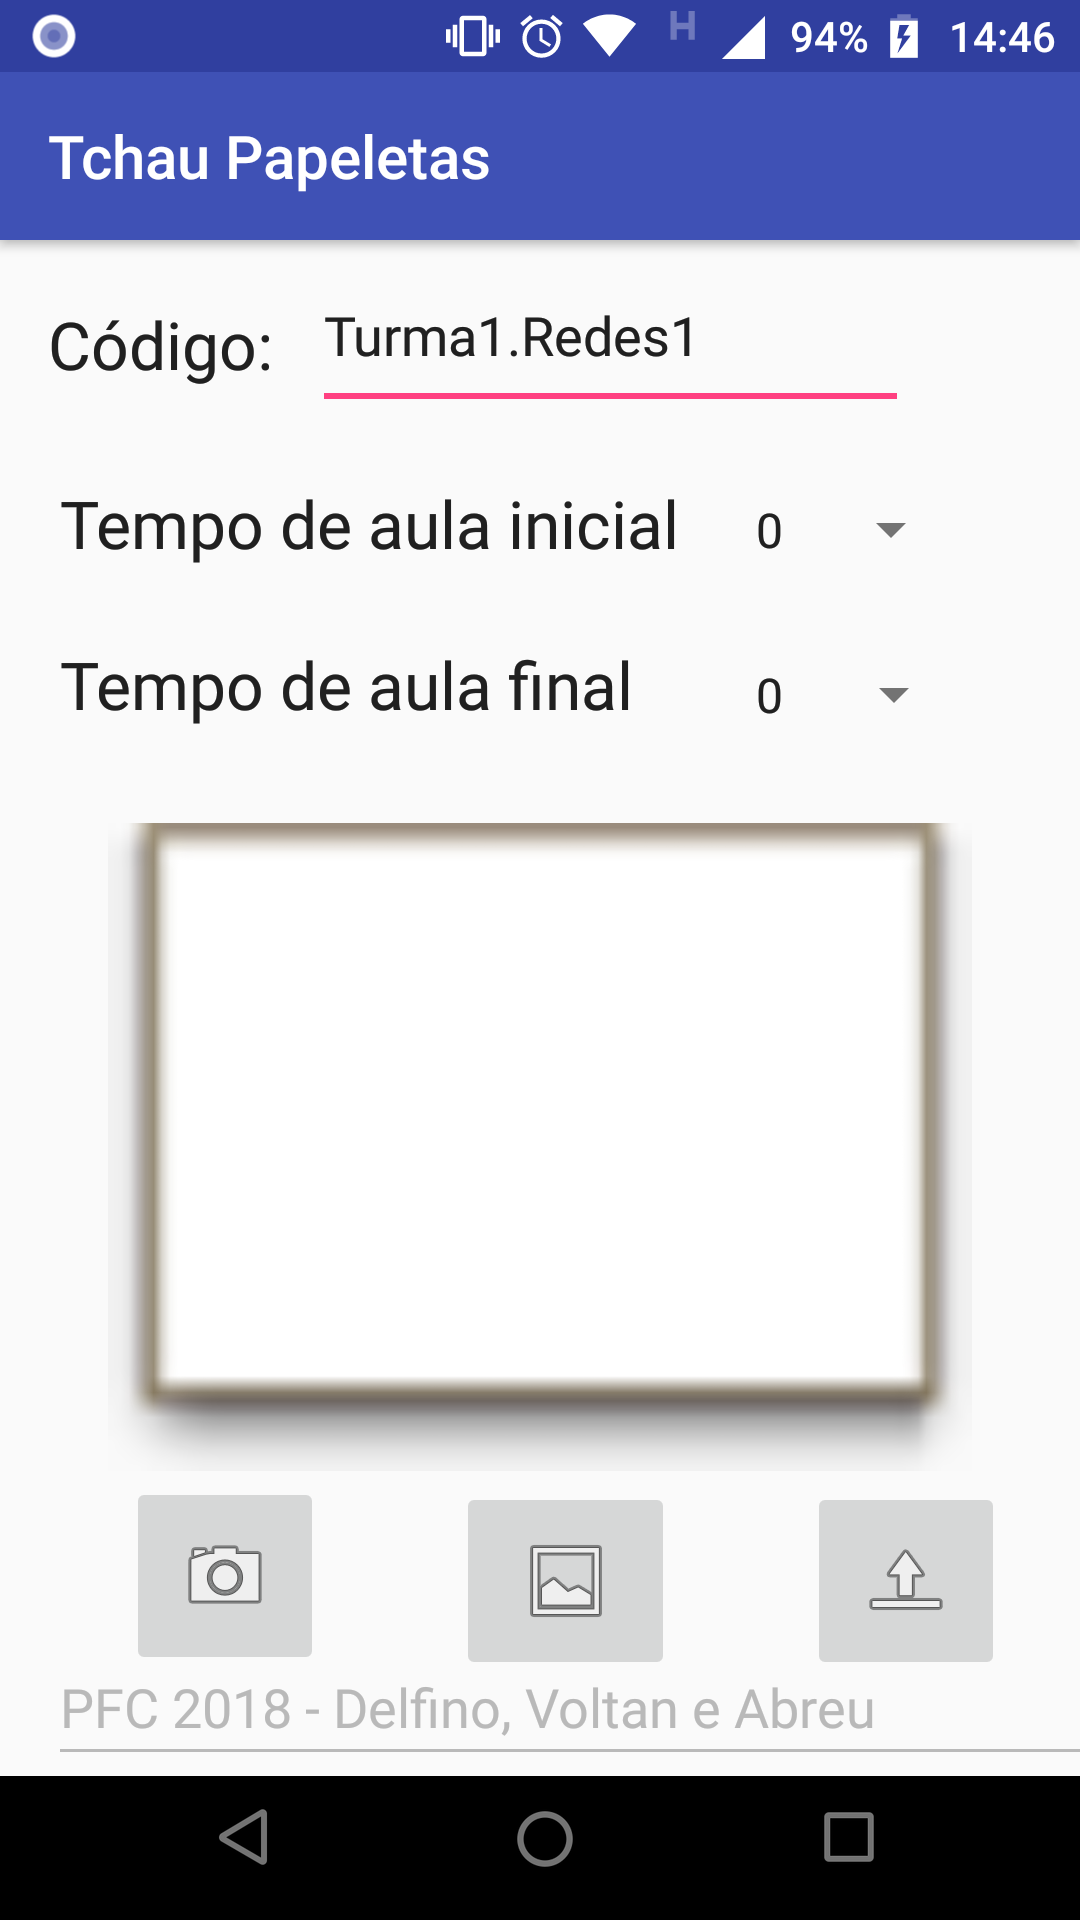
\includegraphics[width=0.3\textwidth]{C_digo_preenchido.png}   
	\caption{Código preenchido}
	\label{fig:figura66}
\end{figure}

No atual momento de desenvolvimento optou-se por deixar esse campo com preenchimento livre de tal forma a possibilitar utilização por qualquer turma e qualquer disciplina, não o limitando a escolhas restritas das disciplinas de alguma seção de ensino, por exemplo. O objetivo é tornar o aplicativo compatível com futuras aplicações e diferentes turmas e disciplinas.


\subsection{Preenchimento do tempo de aula}
O preenchimento dos tempos de aula ocorre clicando sobre os tempos de aula correspondentes, figura \ref{fig:figura57b}. Como os tempos de aula possíveis já estão previamente definidos, optou-se por realizar o preenchimento desse campo através de um controle giratório. Basta clicar na opção desejada para o tempo de aula, quando abrir-se-ão opções de tempos do 1 ao 11, intervalo de horário máximo segundo quadro de horários vigente no IME. 

\begin{figure}[!ht]
	\centering
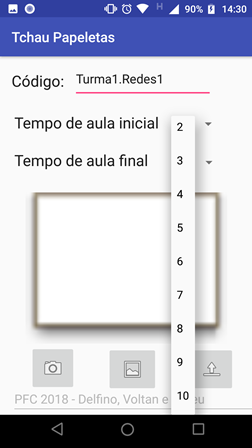
\includegraphics[width=0.3\textwidth]{preenchimento_tempo_de_aula.png}   
	\caption{Preenchimento Tempo de aula}
	\label{fig:figura57b}
\end{figure}

\subsection{Aquisição da imagem}
A aquisição da imagem pode ser feita de duas maneiras diferentes:

• Por meio do acesso à galeria de imagens do dispositivo; ou

• Por meio da captura de uma imagem através da câmera do dispositivo.

\subsubsection{Câmera}
Para iniciar abertura da câmera basta clicar sobre o ícone da câmera. A interface de câmera do sistema operacional Android vigente então abrirá, permitindo a retirada de fotos já familiar ao usuário. Após retirada da foto, o usuário terá opção de confirmar ou rejeitar a foto obtida, figura \ref{fig:figura59b}. Exibir-se-á na tela inicial da aplicação, então, a foto tirada, caso essa tenha sido aprovada pelo usuário.

%\begin{figure}[!ht]
%	\centering
%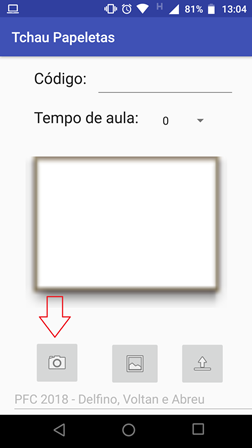
\includegraphics[width=0.3\textwidth]{Icone_1.png}   
%	\caption{Ícone câmera}
%	\label{fig:figura68}
%\end{figure}

\begin{figure}[!ht]
	\centering
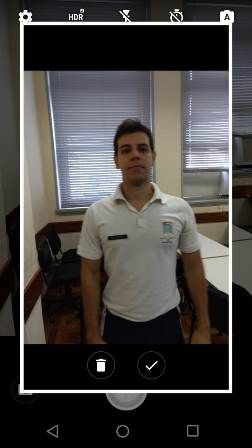
\includegraphics[width=0.3\textwidth]{img/camera_2.jpeg}   
	\caption{Aguardando aprovação da foto tirada}
	\label{fig:figura59b}
\end{figure}

%\begin{figure}[!ht]
%	\centering
%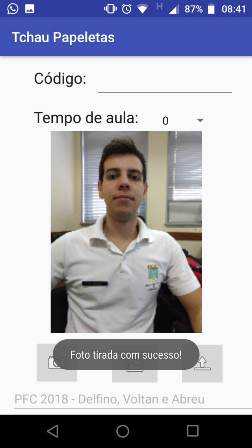
\includegraphics[width=0.3\textwidth]{img/camera_3.jpeg}   
%	\caption{Foto Tirada com sucesso}
%	\label{fig:figura69}
%\end{figure}

\subsubsection{Galeria}
Para iniciar a escolha de foto através da galeria basta clicar sobre o ícone da galeria. A interface de galeria do sistema operacional Android vigente então abrirá, permitindo a escolha de fotos já familiar ao usuário, conforme ilustrado na figura \ref{fig:figura71}. Exibir-se-á na tela inicial da aplicação, então, a foto selecionada pelo usuário. Um exemplo de exibição da foto escolhida na tela inicial da aplicação pode ser vista na figura \ref{fig:figura81}. 
%\begin{figure}[!ht]
%	\centering
%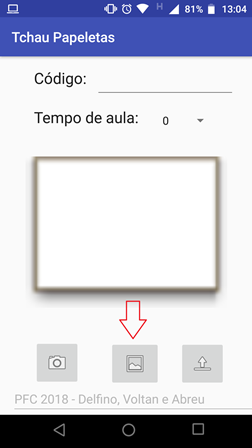
\includegraphics[width=0.3\textwidth]{img/Icone_2.png}   
%	\caption{Ícone galeria}
%	\label{fig:figura70}
%\end{figure}

\begin{figure}[!ht]
	\centering
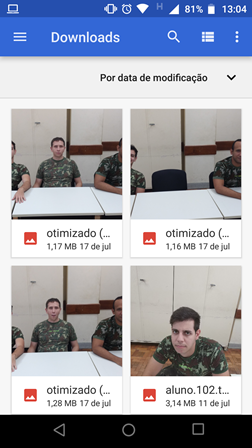
\includegraphics[width=0.3\textwidth]{img/Galeria.png}  
	\caption{Seleção da foto a partir da galeria}
	\label{fig:figura71}
\end{figure}

\begin{figure}[!ht]
	\centering
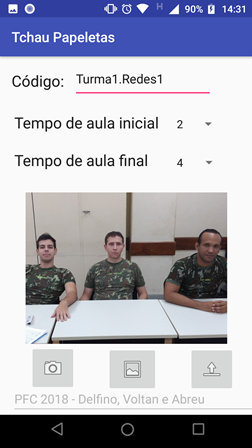
\includegraphics[width=0.3\textwidth]{img/foto_selecionada_com_sucesso.png}  
	\caption{Foto selecionada com sucesso}
	\label{fig:figura81}
\end{figure}

\subsection{Upload para o servidor}
Para enviar todos os dados para o servidor, basta clicar no ícone de \textit{upload}. A aplicação enviará toda a informação coletada caso todos os campos tenham sido preenchidos de maneira adequada. Na impossibilidade dos dados serem aprovados, a aplicação notificará o usuário por meio de notificações qual campo está impossibilitando o sucesso da execução, conforme mostram as figuras \ref{fig:figura73}, \ref{fig:figura74} e \ref{fig:figura75}.

%\begin{figure}[!ht]
%	\centering
%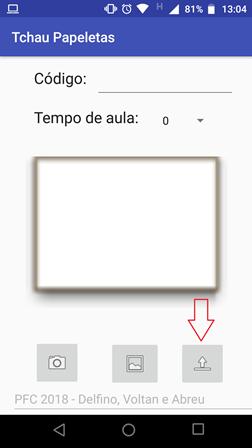
\includegraphics[width=0.3\textwidth]{img/Icone_3.png}   
%	\caption{Ícone upload}
%	\label{fig:figura72}
%\end{figure}
\begin{figure}[!ht]
	\centering
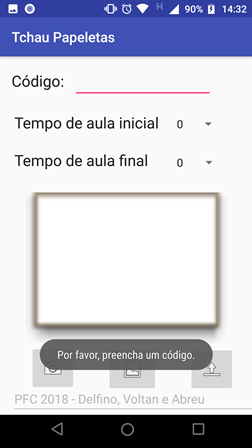
\includegraphics[width=0.3\textwidth]{toast_codigo.png}   
	\caption{Erro no preenchimento do código}
	\label{fig:figura73}
\end{figure}

\begin{figure}[!ht]
	\centering
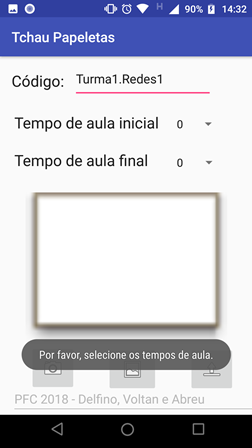
\includegraphics[width=0.3\textwidth]{toast_tempo_de_aula.png}   
	\caption{Erro no preenchimento do tempo de aula}
	\label{fig:figura74}
\end{figure}

\begin{figure}[!ht]
	\centering
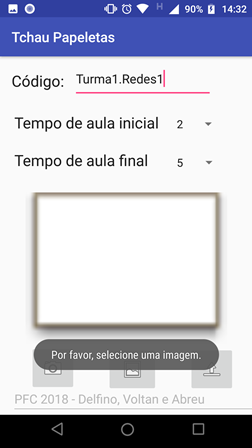
\includegraphics[width=0.3\textwidth]{toast_imagem.png}   
	\caption{Erro na seleção de Imagem}
	\label{fig:figura75}
\end{figure}

Caso todas as informações tenham sido preenchidas corretamente, notificar-se-á o usuário do upload feito de maneira correta, de maneira temporária e também de maneira persistente, figura \ref{fig:figura76}. Além disso, não mais se exibirá a foto enviada, garantindo a percepção de que aquela foto já foi enviada para o servidor, impedindo assim que o professor persista na tentativa de enviar a mesma informação de maneira duplicada.

\begin{figure}[!ht]
	\centering

\includegraphics[width=0.3\textwidth]{upload_sucesso.png}   
	\caption{Upload efetuado com sucesso}
	\label{fig:figura76}
\end{figure}
\newpage
%Após conclusão do módulo 3, módulo do banco de dados, estudar-se-á a exibição dos resultados produzidos pelo reconhecimento facial. O módulo 3 também será o responsável pelo armazenamento persistente dessas informações no banco de dados.

No módulo 3, módulo do banco de dados, estudar-se-á a exibição dos resultados produzidos pelo reconhecimento facial. O módulo 3 também será o responsável pelo armazenamento persistente dessas informações no banco de dados.

\section{Especificações do envio}
O envio das informações dar-se-á através de um \textit{socket}, um ponto final de comunicação entre duas máquinas. Para o caso do trabalho em tela, o \textit{smartphone} utilizado pelo professor contendo a aplicação instalada, cliente, e o computador contendo o servidor. 

Utilizar-se-á o protocolo TCP para a transmissão. A escolha pela não utilização do \textit{DatagramSocket}, que utilizaria o protocolo UDP, deu-se fundamentalmente pela verificação de envio correto das informações presente na utilização do protocolo TCP \citep{Android10}. Apesar de possibilitar um envio mais rápido, o UDP não é confiável, já que não há garantia que o pacote chegou ao destino da maneira correta, fator impeditivo para seu uso na aplicação em questão \citep{Android9}. Além disso, o ganho de desempenho proporcionado pelo protocolo UDP não é almejado com afinco, visto que enviar-se-á uma foto única, não executando uma transmissão contínua de vídeo, por exemplo, ou seja, não necessita de alta taxa de transmissão \citep{Android9}.

Todas as informações serão enviadas através de uma mensagem única. Para isso, converter-se-á a imagem selecionada. Para isso, criar-se-á o arquivo \textit{Bitmap} da foto da turma especificada, obtida por meio da galeria ou captura de câmera. Tal arquivo será, então, convertido em uma stream de dados, utilizando o formato JPEG para a compressão em um \textit{array} de \textit{bytes}. A escolha do formato JPEG deu-se fundamentalmente por ser permitido definir a qualidade de imagem após conversão, especificada como máxima e permitindo o reconhecimento abordado ao longo do capítulo 4. A informação agora escrita nesse \textit{array} de \textit{bytes} é finalmente convertida em base 64 como uma \textit{string}, para ser adicionada a mensagem enviada pelo \textit{socket}, conforme já mencionado. Por fim, enviar-se-á a mensagem contendo as \textit{strings} de Código, Tempo de aula e Foto convertida em \textit{String}, sendo essas informações separadas por vírgula e incluídas nessa ordem em uma padronização exigida para restauração das imagens uma vez que essas sejam recebidas no Servidor TCP. A decodificação realizada no Servidor TCP exige tal padronização.

\subsection{Cliente TCP}
A execução da tarefa em Android é feita por uma instância da classe \textit{SocketImpl}, através da importação do pacote java.net.Socket. A extensa documentação a respeito da utilização de socket em plataformas android no site oficial de referências, \citep{Android10},  bem como o cumprimento de todos os requisitos propostos para o trabalho foram decisivas para a escolha do método de transmissão.


\subsection{Servidor TCP}
O servidor TCP fará a coleta da informação recebida, separando os dados recebidos e convertendo a imagem recebida para o formato o JPEG, já colocando toda a informação necessária no nome do arquivo criado, seguindo as padronizações especificadas ao longo do módulo 4. 
Optou-se por manter a mesma linguagem de programação utilizada para o desenvolvimento da aplicação Android, buscando manter a coerência dentro do módulo desenvolvido. Assim sendo, toda a aplicação do servidor TCP, que conta com interface gráfica, foi desenvolvida em linguagem de programação Java.

Após clicar em "Iniciar serviço", o servidor TCP atuará de maneira contínua, esperando o recebimento de solicitações feitas através da aplicação e salvando as respectivas imagens com os respectivos códigos associados, conforme ilustrado nas figuras \ref{fig:figura77}, \ref{fig:figura78} e \ref{fig:figura79}. Nenhuma ação é necessária para o recebimento das futuras imagens, sendo o processo de decodificação e posterior registro em disco da imagem recebida com o respectivo nome identificador contínuo.

\begin{figure}[!ht]
	\centering
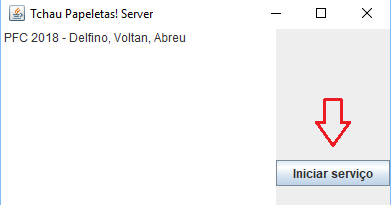
\includegraphics[width=0.5\textwidth]{iniciar_conex_o_1.png}   
	\caption{Iniciando serviço: Passo 1}

	\label{fig:figura77}
\end{figure}
\begin{figure}[!ht]
	\centering
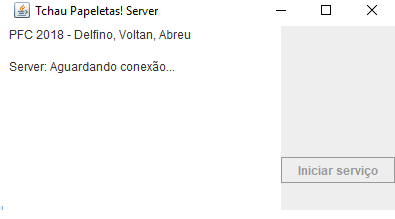
\includegraphics[width=0.5\textwidth]{img/iniciar_conex_o_2.png}   
	\caption{Iniciando serviço: Passo 2}
	\label{fig:figura78}
\end{figure}

\begin{figure}[!ht]
	\centering
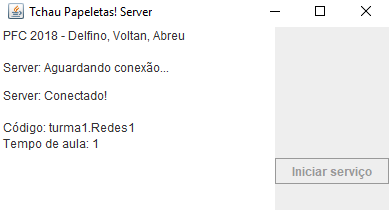
\includegraphics[width=0.5\textwidth]{img/iniciar_conex_o_3.png}   
	\caption{Iniciando serviço: Passo 3}
	\label{fig:figura79}
\end{figure}

\noindent 

\chapter{Módulo BD}
\noindent
Este capítulo tem o objetivo de abordar o último módulo desenvolvido para atender o objetivo proposto: o módulo do BD. Ele é responsável por oferecer o armazenamento persistente ao sistema e sua edição, possibilitando a visualização das faltas e sua alteração. As atividades de consulta e alteração da papeleta são realizadas através de um servidor web, desenvolvido nesse último módulo. Ele está relacionado aos requisitos funcionais \textit{RF02 - Verificar lista de presença} e   \textit{RF03 - Editar lista de presença}. Sobre o banco de dados a ser empregado, o \textit{RN02 - O banco de dados, no qual se fará o armazenamento persistente, deve ser PostgreSQL} torna isso claro. Além disso, o módulo encontra-se relacionado com os 3 casos de uso \textit{UC-01 Apurar falta, UC-02 Editar Lista de presença, UC-03 Verificar Lista de Presença}.

\section{Conceito Geral do módulo}
\noindent
Segundo \citep{bd}, os bancos de dados e suas tecnologias representam um papel crítico nos mais diversos sistemas nos quais se inserem, sendo que o nome banco de dados está relacionado a um conjunto de dados relacionados. No sistema proposto, esse conjunto de dados seria a composição das informações relacionadas à presença dos alunos, ou seja, disciplina, tempo de aula, matrícula do aluno, entre outros.

O banco de dados escolhido foi o \textit{PostgreSQL}, visando atender ao RN02 que estabelece que "o banco de dados, no qual se fará o armazenamento persistente, deve ser PostgreSQL". Segundo \citep{postsql}, o \textit{PostgreSQL} é um banco de dados relacional, com código aberto e que usa e estende a tradicional linguagem SQL. Ele teve origem na Universidade da Califórnia em Berkeley, no ano de 1986. Nesse contexto, o banco de dados relacional conta com mais de 30 anos de desenvolvimento e aperfeiçoamento. A versão escolhida foi a 9.6.10. Optou-se por utilizar o \textit{pgAdmin III}, em sua versão 1.22.2. O \textit{pgAdmin III}, segundo \citep{pgadmin}, é uma ferramenta para o gerenciamento de banco de dados \textit{PostgreSQL} que possui interface gráfica e ferramentas que auxiliam no gerenciamento e manutenção do banco. Sobre a licença, \citep{pgadmin} informa que a ferramenta é disponibilizada gratuitamente. 


\section{Modelagem do Banco de Dados}
\noindent 
O Modelo Entidade-Relacionamento, segundo \citep{bd}, é um modelo conceitual, muito popular, que trabalha com uma abstração de alto nível, empregando entidades, relacionamentos e atributos em sua modelagem.\citep{bd} explica ainda que o Diagrama Entidade-Relacionamento (ER) é a representação gráfica para um esquema. Buscou-se modelar um banco de dados de maneira simplificada, mas que atenda ao propósito do sistema de registrar a apuração das faltas por tempo de aula. Para a construção do Diagrama ER, utilizou-se o software brModelo 3.0. \citep{brmodelo} informa que ele foi desenvolvido por Carlos Henrique Cândido, e trata-se de uma ferramenta para a modelagem relacional. Destaca-se o fato do software desenvolvido por Carlos Cândido ser nacional e gratuito.    

A figura \ref{fig:figura60aa} ilustra o Diagrama ER para o sistema. Nele, tem-se as entidades \textit{aluno, turma, disciplina, professor, aula}. Cada aluno está matriculado em uma turma e cada turma cursa uma disciplina. Cabe aqui observar que, no Instituto Militar de Engenharia, os alunos devem cursar, obrigatoriamente, as disciplinas previstas para aquele semestre. Assim sendo, uma turma tem sua grade  de disciplinas rígida, tendo sido determinadas previamente as disciplinas a serem cursadas em um dado semestre. Um ou mais professores podem ministrar uma disciplina ao longo do semestre. Ao evento específico no qual um professor ministra uma disciplina, durante um intervalo predefinido de tempo, deu-se o nome de aula. Optou-se por considerar aula como sendo uma entidade devido à ênfase do sistema. Por fim, o aluno pode comparecer a uma aula ou não. Pode-se notar que aluno e professor guardam certa semelhança, sendo possível para ambos herdarem da entidade pessoa, o que não foi feito no diagrama apenas com a finalidade de torná-lo mais legível. Quanto a cardinalidade do relacionamento, optou-se por seguir a terminologia proposta por \citep{bdcardinalidade}, por exemplo, um aluno está matriculado em uma única turma, podendo uma turma ter um ou mais alunos. 

\begin{figure}[!ht]
	\centering
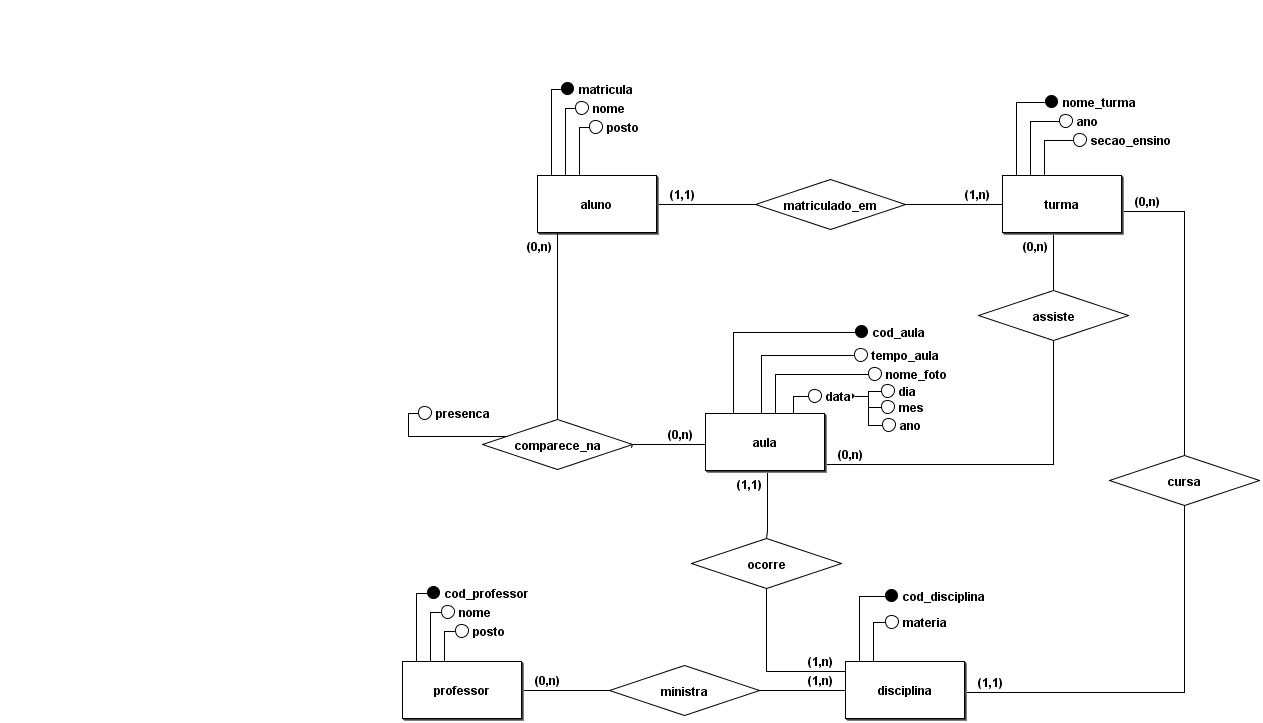
\includegraphics[width=1\textwidth]{img/Conceitual_1.png}   
	\caption{Diagrama ER do sistema}
	\label{fig:figura60aa}
\end{figure}


Na fase seguinte, usando o modelo ER, construiu-se o modelo de dados relacional. \citep{bd} explica que esse modelo trata o banco de dados como sendo um conjunto de relações. Representou-se através da figura  \ref{fig:figura60ab} o Diagrama para o esquema do banco de dados relacional tchau\_papeleta.  Quanto ao formato da representação, adotou-se o que \citep{bd} sugere em seu capítulo 5, página 98.  

\begin{figure}[!ht]
	\centering
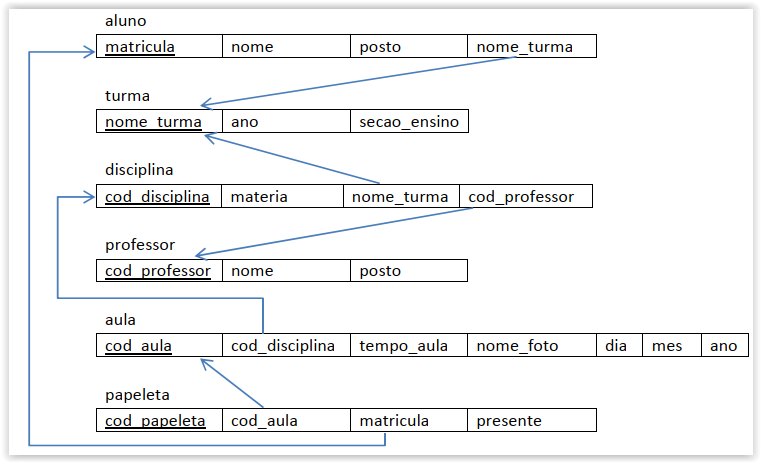
\includegraphics[width=1\textwidth]{img/relacional.PNG}   
	\caption{Diagrama para o esquema do banco de dados relacional tchau\_papeleta}
	\label{fig:figura60ab}
\end{figure}

\section{Criação do esquema}
Na fase seguinte, criou-se um banco de dados relacional do tipo postgreSQL. No banco de dados proposto, a tabela \textbf{aluno} tem as colunas matrícula, nome, posto e cod\_turma. A matrícula, por ser um identificador único, é a chave primária. Para a coluna posto, os alunos militares têm a abreviação de sua graduação ou posto. Os alunos da reserva receberiam a palavra \textit{civil}. O nome\_turma faz referência à turma, sendo uma chave estrangeira. A \textbf{turma} seria composta pelo nome\_turma, um identificador único da turma que funciona como chave primária, além do ano e da secao\_ensino. O ano se refere ao ano da graduação na qual a turma se encontra e.g: o 5º ano teria ano igual a 5. A secao\_ensino representa a seção de ensino, sendo essa uma sigla sigla, e.g: SE8. O \textbf{professor} é composto por um cod\_professor, chave primária, além do nome e posto. A \textbf{disciplina} é formada por cod\_disciplina, matéria (nome por extenso da disciplina), nome\_turma (chave estrangeira fazendo referência à turma), cod\_professor1 e cod\_professor2 (chaves estrangeiras que referenciam  professor). Nesse momento, vale destacar que preferiu-se utilizar 2 campos para professor, priorizando o desempenho ao espaço, isso se explica pois no IME, as disciplinas tem, em geral, no máximo 2 professores encarregados de uma disciplina. Criar uma tabela relacionando professor e disciplina, nesse caso teria um impacto negativo no desempenho, e traria um benefício de evitar redundância pequeno. A \textbf{aula} é composta por cod\_aula (chave primária), dia, mês e ano (compondo a data), cod\_disciplina (chave estrangeira que se refere à disciplina), tempo\_aula e nome\_foto. Por fim, a \textbf{papeleta} é composta por cod\_papeleta (chave primária), cod\_aula (chave estrangeira que refere aula), matrícula (chave estrangeira que refere aluno). Além desses, ter-se-á a coluna presente, um \textit{boolean} no qual  \textit{true} representa que o aluno compareceu à aula e  \textit{false} que o aluno faltou.

Criou-se um \textit{Database} denominado IME. A partir dele, criou-se o esquema e suas tabelas. A figura \ref{fig:figura60a} mostra a criação do esquema denominado \textit{tchau\_papeleta}. A seguir, as tabelas \textit{turma, aluno, professor, disciplina, aula e papeleta} são criadas. Após a criação do esquema e tabelas, fez-se a inserção de dados, conforme ilustrado na figura \ref{fig:figura61a}. Para o funcionamento do sistema, os professores, alunos, disciplinas e turmas já devem ter sido previamente cadastrados, conforme ilustra a figura \ref{fig:figura61a}.  

\begin{figure}[!ht]
	\centering
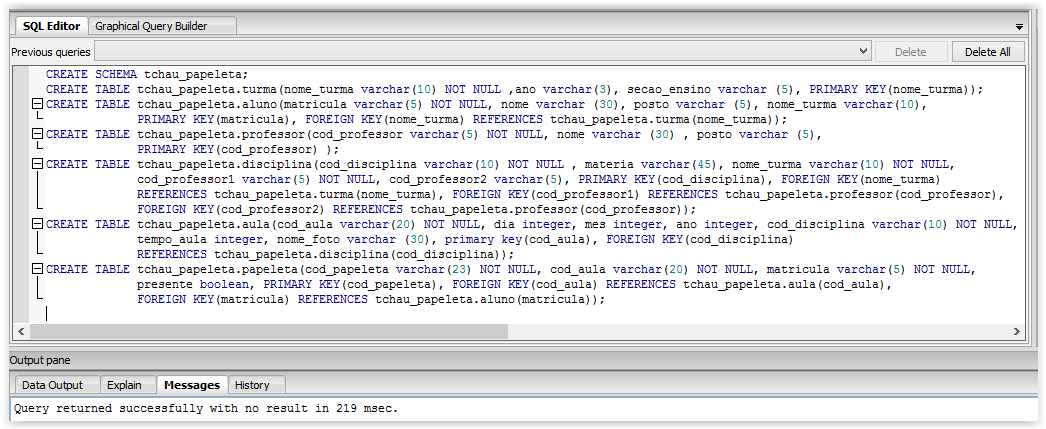
\includegraphics[width=1\textwidth]{scriptcriacao.PNG}   
	\caption{Criação usando o pgAdmin III}
	\label{fig:figura60a}
\end{figure}

\begin{figure}[!ht]
	\centering
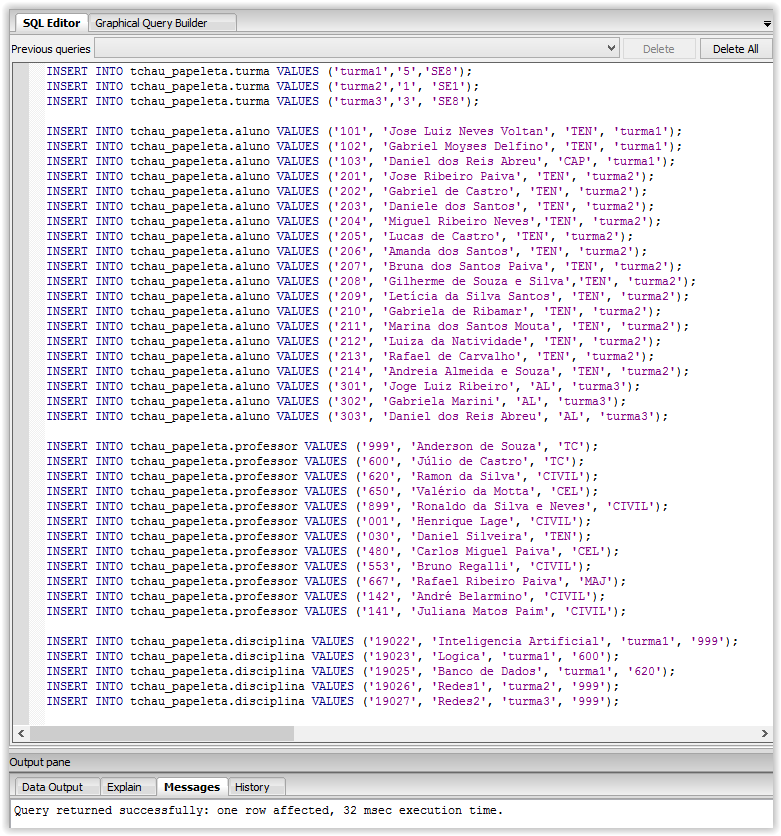
\includegraphics[width=1\textwidth]{populacao.PNG}   
	\caption{Inserção dos dados no esquema \textit{tchau\_papeleta}}
	\label{fig:figura61a}
\end{figure}

Quando o professor, utilizando o aplicativo "Tchau Papeletas", fizer o envio da fotografia da turma, ele também enviará nome da turma, representado no esquema como \textit{nome\_turma}, e o nome da disciplina, que aparecerá como \textit{materia}. Essas duas informações serão necessárias para identificar a turma de maneira inequívoca, uma vez que  uma mesma matéria pode ser oferecida para mais de uma turma. Por exemplo, a matéria "Fenômenos de Transporte" é ministrada com o mesmo nome tanto para o 3º ano de Engenharia Química quanto para o 3º ano de Engenharia da computação. Trata-se, contudo, de disciplinas distintas, com códigos (\textit{cod\_disciplina}) e conteúdo diferentes. A figura \ref{fig:figura62a} exibe a consulta para, a partir dessas duas informações, encontrar-se o \textit{cod\_disciplina}. No exemplo, \textit{nome\_turma} = 'turma1' e \textit{materia} = 'Logica', retornando como resultado o \textit{cod\_disciplina} = 19023.

\begin{figure}[!ht]
	\centering
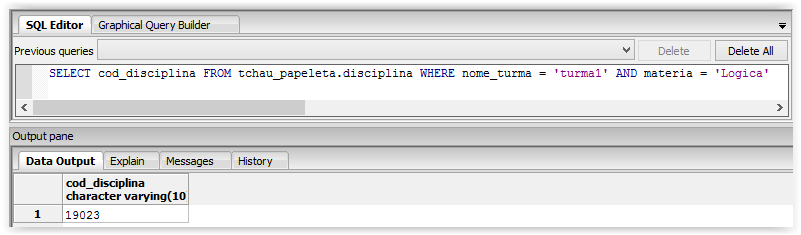
\includegraphics[width=1\textwidth]{consulta1.PNG}   
	\caption{Consulta para obtenção da \textit{cod\_disciplina}}
	\label{fig:figura62a}
\end{figure}

Além desses, o professor também informará os tempo de aula, sendo a data composta por dia, mês e ano incluída pelo servidor. Com essas informações, ter-se-á parâmetros suficientes para criação da aula. A figura \ref{fig:figura63a} demonstra a inserção de uma aula ministrada no dia 05, mês 09 e ano 2018, referente à disciplina Lógica, ministrada para a turma1, (\textit{cod\_disciplina} = '19023'). Preencher-se-á o atributo \textit{nome\_foto} conforme apresentado no capítulo 4, referente ao módulo servidor. 

\begin{figure}[!ht]
	\centering
\includegraphics[width=1.0\textwidth]{consulta2.PNG}   
	\caption{Inserção de uma aula}
	\label{fig:figura63a}
\end{figure}

Após a inserção da aula, pode-se gerar para cada membro da turma a presença ou falta naquela aula. A figura \ref{fig:figura64a} mostra como obter a \textit{matrícula} dos alunos de uma turma. No exemplo, utiliza-se turma1. Por fim, a figura \ref{fig:figura65a} demonstra a inserção da presença ou falta de cada aluno dessa turma.  

\begin{figure}[!ht]
	\centering
\includegraphics[width=1.0\textwidth]{consulta3.PNG}   
	\caption{Obtenção da relação de aluno (\textit{matrícula}) de uma turma}
	\label{fig:figura64a}
\end{figure}

\begin{figure}[!ht]
	\centering
\includegraphics[width=1.0\textwidth]{consulta4.PNG}   
	\caption{Inserção da falta}
	\label{fig:figura65a}
\end{figure}


\section{Conexão com o Banco de Dados através do Python DB API}
Depois que a fotografia é enviada para o servidor e  as faces são reconhecidas, registrar-se-á essas informações no banco de dados. Para a integração entre o código escrito em Python e o PostgreSQL, fez-se uso do \textit{Psycopg}. Segundo \citep{Psycopg}, o \textit{Psycopg} é o adaptador mais popular para essa finalidade. O \textit{"Python DB API 2.0"} possui licença gratuita e segue a política \textit{GNU Lesser General Public License}. A versão escolhida foi a 2.7.5. 

Optou-se, então, por criar uma classe denominada Conecta (arquivo conexao.py), que apresenta os métodos necessários para a manipulação dos dados. Em seu construtor, realizar-se-á a conexão com o banco de dados, usando como parâmetros \textit{host, database, usuário} e \textit{senha}. A classe possui ainda, dentre outos, os métodos genéricos para consulta e inserção (cláusulas \textit{select} e \textit{insert}). 

Quando uma fotografia de uma turma é recebida, o primeiro passo é identificar se aquela fotografia é a primeira ou não. Caso seja a primeira, deve-se criar a linha aula correspondente àquela fotografia e suas informações, além da papeleta de cada aluno com o atributo presente recebendo \textit{false}. Caso não seja a primeira isso não deve ser feito sob pena de apagar a presença de um aluno apurada anteriormente. Para essa verificação, optou-se por, dentro do método \textit{inserir\_aula}, consultar se, de fato, aquela inserção é necessária ou não. Caso necessário, além da inserção, cria-se a papeleta de cada aluno como mencionado. O retorno do referido método é o \textit{cod\_aula}.  O passo seguinte é criar um método nessa classe tal que, recebendo a matrícula do aluno que teve sua face detectada, seja permitido alterar, na linha correspondente da tabela papeleta, o atributo presente de \textit{false} para \textit{true}. 

\section{Acesso ao Banco de Dados para Consulta e Atualização}
Para o atendimento dos requisitos RF02 e RF03, definidos no capítulo de modelagem do sistema, foi implementado um serviço \textit{web}, no qual o cliente consiste em um formulário HTML e o servidor em uma página JSP. No formulário, constam os seguintes campos de preenchimento: dia, mês, ano, tempo de aula, turma e disciplina . Com essa informação é possível fazer uma consulta que retorna a matrícula, o posto e o nome de todos os alunos da turma, bem como a situação de cada um quanto a frequência ao tempo de aula especificado. 
A estrutura desse serviço \textit{web} caracteriza-se por uma página inicial, ilustrada na figura \ref{fig:figura66}, que exibe dois \textit{links} de acesso: 
\textit{Link} de acesso para a atualização, que permite a consulta e atualização do banco de dados, isso é, os dados são exibidos na forma de uma tabela e o usuário pode alterar a presença ou falta do aluno; e
\textit{Link} que permite apenas consulta, voltado para alunos e coordenadores.
Ambos os \textit{links} direcionam o usuário para a página que contém o formulário, figura \ref{fig:figura67}, o qual, ao ser enviado, direciona para a página JSP, que se encarrega de fazer a manipulação do banco de dados, conforme mostra a figura \ref{fig:figura68}. Caso o formulário seja enviado pelo professor, o servidor exibe uma tabela com o resultado da consulta e contendo uma coluna com botões cuja função é modificar a situação do aluno, de presente para ausente ou o inverso. Se for aluno ou coordenador, o servidor retorna retorna a mesma tabela do caso anterior, porém sem as permissões de alteração e exibição dos botões. 
\begin{figure}[!ht]
	\centering
\includegraphics[width=0.70\textwidth]{img/home_page.png}  
	\caption{Página inicial do serviço(\textit{web})}
	\label{fig:figura66}
\end{figure}

\begin{figure}[!ht]
	\centering
\includegraphics[width=0.70\textwidth]{img/pagina_de_consulta.png}   
	\caption{Página de preenchimento e envio de formulário html}
	\label{fig:figura67}
\end{figure}

\begin{figure}[!ht]
	\centering
\includegraphics[width=0.70\textwidth]{img/servidorjsp.png}   
	\caption{Página de exibição do resultado da operação Atualização}
	\label{fig:figura68}
\end{figure}


Conforme mencionado anteriormente, a transação de atualização é feita pelos botões. Cada botão, ao ser pressionado, atualiza a frequência da linha a qual se refere. Quando a operação é bem sucedida, o usuário é notificado do sucesso por uma mensagem de texto, exibida abaixo da tabela, e também pela mudança de cor do campo presença e do próprio botão acionado. É importante mencionar que durante essas atualizações e notificações a página não precisa ser recarregada, evitando-se, assim, a necessidade de uma nova consulta para obter a tabela a cada atualização feita. Isso é possível por meio de requisições HTTP assíncronas, conhecidas como AJAX, que permitem a troca de dados entre cliente e servidor em segundo plano e a atualização de partes da página sem a necessidade de recarregar a página como um todo, \citep{W3}. A figura \ref{fig:figura69} mostra um exemplo de notificação. 

\begin{figure}[!ht]
	\centering
\includegraphics[width=0.70\textwidth]{img/atualizacao.png}   
	\caption{Exemplo de atualização}
	\label{fig:figura69}
\end{figure}

Perceba que devido à questões temporais limitantes do projeto, não se projetou um sistema de autenticação de usuário. Como oportunidade de melhoria, pode se ter um cadastro com login e senha dos usuários, que permita a separação das operações conforme a função do usuário, assim um aluno não poderia atualizar a lista de presença de uma turma, mas um professor sim. Além disso, poderia se dar um tratamento especial aos campos, evitando tentativas de injeção SQL. 







\chapter{Análise crítica do sistema}
\noindent
Realizar-se-á nesse capítulo uma análise crítica do sistema, verificando primeiramente se todos os requisitos propostos foram satisfatoriamente atendidos e, posteriormente, analisando oportunidades de melhoria para futuros projetos que tenham como base temas próximos ao do trabalho em tela. 
\section{Verificação dos requisitos}
Cabe, nesse momento, verificar se os requisitos levantados no início do projeto (Capítulo 3) foram satisfatoriamente atendidos.
\subsection{Requisitos funcionais}
Tratar-se-á primeiro sobre os requisitos funcionais:
\begin{itemize}
\item RF01 - Apurar falta; 
\item RF02 - Verificar lista de presença; 
\item RF03 - Editar lista de presença; e 
\item RF04 - Armazenar fotografia.
\end{itemize}

Após o envio da fotografia da turma, e recebimento pelo servidor tem-se a apuração das faltas. Vale destacar que a fotografia é selecionada pelo professor a partir do acesso à sua galeria ou obtida através da câmera no momento de aula. A análise da foto permite identificar as faces do alunos, possibilitando atribuir presença para os alunos reconhecidos no processo. O sistema consegue reconhecer várias faces em uma mesma fotografia, e permite o envio de várias fotografias para um mesmo tempo (em operações de envio distintas). Assim sendo, apura-se satisfatoriamente as faltas e cumpre-se o RF01. 

A verificação da lista de presença é possível devido ao módulo BD, que busca, no banco de dados, as informações referentes a presença e as exibe no ambiente Web, permitindo consulta. Além disso, o módulo BD também permite, através da interface web, que a presença em uma papeleta de faltas seja editada. Cumpre-se, dessa maneira, os requisitos RF02 e RF01. Cabe mais uma vez destacar a limitação mencionada ao final do capítulo 6. Por questões de limitações temporais do projeto, não foi projetado um sistema de login e senha. Com o sistema atual o professor pode fazer a edição/atualização da papeleta, com um sistema de login e senha, com um sistema de login e senha, somente o professor poderia fazer essa edição/atualização.

Por fim, quando o módulo servidor terminar a análise da fotografia, a mesma será transferida para a pasta de armazenamento (denominada apuradas). Permite-se, assim, uma auditoria no futuro caso essa seja necessária. O armazenamento da fotografia, então, consolida o cumprimento do RF04.

\subsection{Requisitos não funcionais}
Tratar-se-á, agora, os requisitos não funcionais:
\begin{itemize}
\item RN01 - O Sistema deve apresentar interface com o usuário “Professor” compatível com o sistema \textit{Android}; 
\item RN02 - O banco de dados, no qual se fará o armazenamento persistente, deve ser PostgreSQL; 
\item RN03 - As tarefas de captura de foto, reconhecimento facial e armazenamento de registros devem ser feitas em módulos distintos; e
\item RN04 - Um professor deve ser capaz de utilizar o sistema após um treinamento de 15 minutos.
\end{itemize}

Conforme descrito descrito ao longo da descrição da aplicação mobile (Capítulo 5), o aplicativo teve seu desenvolvimento focado no sistema operacional \textit{Android}, satisfatoriamente cumprindo o RN01. De maneira semelhante, desenvolveu-se o armazenamento persistente das informações em banco de dados utilizando PostgreSQL, o que foi descrito ao longo do (Capítulo 6). Como sugestão de melhoria, poderia-se acrescentar ao aplicativo uma tela que redirecionasse para a tela de consulta, dessa forma, após o envio da fotografia, o professor já iria observar quais alunos foram reconhecidos e quais não, e assim optar por enviar uma nova fotografia ou simplesmente atualizar a papeleta.

Quanto a modularização, tem-se que a leitura do trabalho torna claro o fato de que a realização do projeto foi inteiramente feita de maneira modular. Isso permite que trabalhos futuros reaproveitem o projeto, substituindo apenas alguns módulos. Assim sendo, concluí-se que o RN03 também foi atendido.

Por fim, a interface amigável das aplicações \textit{Android} e \textit{Web} tornam a utilização de todo o sistema extremamente intuitiva. Dessa forma, garante-se que a utilização do sistema não apresentará dificuldades para maior parte do grupo de utilizadores mesmo dentro do contexto da utilização acontecer sem nenhum treinamento prévio. Além disso, espera-se que, em uma eventual necessidade, dúvidas sobre a utilização do sistema por determinado professor possam ser sanadas em um tempo inferior a 15 minutos. Garante-se, assim, o cumprimento do RN04.

\section{Oportunidades de melhoria}
Entende-se que o módulo de reconhecimento facial, apresentado ao longo do capítulo 4, pode ser modificado de tal forma a melhorar os índices de reconhecimento, ou seja, pode-se buscar apurar as faltas com mais eficiência a partir da fotografia analisada. A utilização da biblioteca \textit{OpenCV}, biblioteca gratuita para uso no meio acadêmico e comercial, foi satisfatória para os objetivos do trabalho em tela, mas pode-se explorar formas de melhorar os algoritmos, sendo o \textit{HaarCascade} ou até mesmo o LBPH. Essa melhoria de algoritmos, que fugiria do escopo do trabalho em tela, pode resultar em melhores índices no número de faces reconhecidas e também em uma maior certeza associada a cada um dos reconhecimentos.

Entende-se também que fotografar a turma pode ser uma tarefa demandadora de tempo. Tal ação poderia ser substituída por um sistema automático de retirada de fotos. Uma câmera, por exemplo, poderia ser colocada na sala de aula em posição estratégica e, ao longo da aula, fotografar-se-ia os alunos presentes, sempre atribuindo presença aqueles que foram reconhecidos. Nesse contexto, não seria mais responsabilidade do professor fotografar a turma e economizaria-se tempo de aula, já que não seria mais necessário utilizar parte do tempo de aula para enviar a fotografia para o servidor. Destaca-se ainda o fato de que a automatização do processo permitiria que várias fotografias fossem tiradas em diferentes momentos da aula, melhorando os índices de reconhecimento já que criar-se-ia diferentes oportunidades de reconhecimento.

Por fim, destaca-se oportunidades de melhoria da aplicação \textit{Web}, cuja interface gráfica pode ser modificada e cuja segurança de acesso pode ser intensificada. As consequências seriam uma experiência de utilização mais agradável e um aumento de segurança, impedindo, por exemplo, que modificações dos status de presença dos alunos fossem realizados por alguém que não o professor que ministrou a respectiva aulas.

%\\chapter{Utilização e testes do sistema}
%\\noindent
%\Nesse capítulo, realizam-se demonstrações do funcionamento do sistema, buscando mostrar de maneira clara como utilizar o sistema.
%\\section{Conceito Geral do módulo}



%\De fato o sistema atende a todos requisitos funcionais estabelecidos. A apuração das faltas é feita posteriormente ao recebimento da foto, registrada pelo professor ou selecionada à partir da sua galeria. A análise da foto permite identificar as faces do alunos, possibilitando atribuir presença para os alunos reconhecidos no processo. Quanto a verificação da lista de presença, tem-se a realização como possível devido ao módulo BD, que busca, no banco de dados, as informações referentes a presença. Além disso, o módulo BD também permite, através da interface web, que se edite a presença em uma papeleta de faltas. Por fim, quando o módulo servidor terminar a análise da fotografia, migrar-se-á a mesma para a pasta de armazenamento, , permitindo, assim, uma auditoria.
%\begin{itemize}
%\item RF01 - Apurar falta: O sistema deve apurar as faltas de um determinado tempo de aula em uma data, disciplina, para uma turma, usando o reconhecimento facial em uma fotografia da turma. As fotos devem ser tiradas por um dispositivo móvel com câmera ou selecionadas de sua galeria. Deve-se reconhecer várias faces em uma única fotografia, isso é, a fotografia é da turma e não individual. As informações referentes a data, isso é, dia, mês e ano devem ser extraídas do servidor; 

%\item RF02 - Verificar lista de presença : Um aluno, coordenador ou professor deve ser capaz de  exibir a lista de presença referente a um determinado tempo de aula, de um determinado dia para uma turma específica; 
%\item RF03 - Editar lista de presença : O professor deve ser capaz de alterar as faltas de um tempo de aula, isso permite que ele corrija eventuais erros na apuração de faltas que usou o reconhecimento facial; e 
%\item RF04 - Armazenar fotografia : Deve-se armazenar a fotografia com sua apuração, permitindo uma auditoria.
%\end{itemize}
%
%Quanto aos requisitos não-funcionais:
%\begin{itemize}
%\item RN01 - O Sistema deve apresentar interface com o usuário “Professor” compatível com o  sistema Android; 

%\item RN02 - O banco de dados, no qual se fará o armazenamento persistente, deve ser PostgreSQL;

%\item RN03 - As tarefas de captura de foto, reconhecimento facial e armazenamento de registros devem ser feitas em módulos distintos; e

%\item RN04 - Um professor deve ser capaz de utilizar o sistema após um treinamento de 15 minutos.
%\end{itemize}

%O sistema também atende a todos os requisitos acima expostos. O módulo %\textit{mobile} foi construído na forma de um aplicativo Android. O banco de dados utilizado foi o PostgreSQL. Toda construção do sistema seguiu o princípio da modularidade, onde se tem os módulos \textit{servidor, mobile e BD}. Por fim, o aspecto simples e intuitivo do aplicativo Tchau Papeletas combinado com a página de exibição e edição das papeletas permitiram que os professores convidados conseguissem utilizar o sistema com um tempo inferior de treinamento. 
\chapter{Conclusão}
\noindent
Este trabalho teve como objetivo desenvolver um sistema informatizado, que utilizasse o reconhecimento facial em conjunto com a tecnologia de desenvolvimento móvel, capaz de ser uma alternativa para o atual sistema de apuração de faltas dos alunos do IME. Após o estudo conceitual sobre métodos de detecção e reconhecimento facial, foi possível  entender melhor as possibilidades oferecidas pela utilização dos diferentes algoritmos pesquisados. Tal entendimento tornou possível a escolha do algoritmo que melhor atenderia ao objetivo do projeto: o LBPH.

O sistema desenvolvido integra uma aplicação \textit{Android}, um banco de dados, um servidor de reconhecimento facial e  um serviço \textit{web} para a realização da apuração de faltas dos alunos do IME. Apesar de trabalharem para o mesmo objetivo, esses elementos são independentes entre si, de forma que qualquer um deles pode ser modificado ou substituído sem afetar o sistema como um todo. Dessa forma, a manutenibilidade do sistema fica facilitada permitindo que futuros projetos deem continuidade ao estudo e proponham soluções de melhoria a partir do aprimoramento dos módulos conforme a necessidade ou o surgimento de técnicas novas.

Por fim, o resultado alcançado mostrou-se compatível ao objetivo proposto, apresentando uma interface amigável e de rápido entendimento para os usuários . Além disso, funções como a correção da papeleta, realizada pelo serviço \textit{web}, onde o professor pode alterar manualmente a presença de um aluno, ajudam a aumentar a confiabilidade do sistema, uma vez que o reconhecimento facial pode falhar. %Outra função que merece destaque é o armazenamento da fotografia analisada, uma vez que permite a verificação da presença \textit{a posteriori}, caso o aluno conteste sua falta. 

%FUNDAMENTAR ESCOLHA
%Optou-se pelo desenvolvimento em módulos buscando dividir o problema em partes e facilitar a eventual substituição pontual de determinado módulo. Na possibilidade de obter-se um algoritmo de reconhecimento facial com melhor qualidade no futuro, ou seja, com taxas de acerto mais elevadas, o módulo Servidor seria passível de substituição pelo novo a um custo reduzido, por exemplo.

%Por fim, o fato do projeto ter sido desenvolvido de maneira modular permite que futuros projetos deem continuidade ao estudo e proponham soluções de melhoria sem que, para isso, percam a oportunidade de utilizar parte daquilo que já foi desenvolvido.

%No módulo Servidor, escolheu-se o uso da linguagem Python pela sua facilidade de leitura, compreensão e manutenção. Além disso optou-se pela biblioteca OpenCV, que apresenta a implementação do algortimo LBPH. Com base nos testes de reconhecimento facial, utilizando o banco de imagens disponibilizado pela Universidade de Yale \citep{yales}  apresentados no capítulo 4, escolheu-se os parâmetros para o algoritmo LBPH de maneira a obter a maior taxa de acerto possível. 

%No módulo \textit{Mobile}, optou-se pelo sistema Android, desenvolvendo um aplicativo de uso intuitivo. Como abordado ao longo do capítulo 5, a escolha pelo desenvolvimento em Android contribui para a tentativa de tornar o aplicativo tão acessível quanto possível e aumenta a qualidade do produto final pela possibilidade de usar componentes já prontos intrínsecos ao sistema operacional. A linguagem utilizada no desenvolvimento foi a recomendada pela documentação oficial, Java.\citep{Android1} Para manter a coerência de linguagem dentro do módulo, utilizou-se a mesma linguagem na construção do servidor TCP que receberá toda a informação. A escolha pela utilização de socket TCP/IP, também embasada ao longo do capítulo 5, deu-se fundamentalmente pela verificação de envio correto das informações ao utilizar tal protocolo.

%Conluída esta etapa, já é possível que um professor, utilizando o aplicativo, preencha os dados da aula, selecione uma imagem, da galeria ou câmera fotográfica, e envie o pedido de apuração ao módulo Servidor. Dar-se-á, então, inicio à detecção de faces na fotografia  selecionada, reconhecendo cada uma dessas com base no arquivo de treinamento para a turma em questão. Ao final, as informações de quais alunos tiveram sua face detectada serão exibidas na tela do servidor, adicionando-se também a matrícula dos alunos em cada uma das faces da fotografia enviada.

%Após o estudo conceitual sobre métodos de detecção e reconhecimento facial, foi possível  entender melhor as possibilidades oferecidas pela utilização dos diferentes algoritmos pesquisados. Tal entendimento tornou possível a escolha daquele  algoritmo que melhor atenderia os objetivos propostos: o LBPH.

%A escolha foi feita principalmente devido ao baixo valor de distância entre as fotos analisadas durante os testes, ou seja, na certeza obtida na detecção de cada uma das faces em teste. Considerou-se essa característica como fundamental pois é imprescindível ou determinar com precisão quem é o aluno presente ou reconhecer que não se tem essa informação com uma precisão satisfatória. Usando então valores adequados para o parâmetro de distância máxima permitida, \textit{threshold}, busca-se evitar dar presença para um aluno que não está em sala ao invés de se dar presença para aquele aluno que estava em sala, i.e. confundir dois alunos. 

%Além disso, ficou claro que o processamento de detecção e o arquivo de inteligência necessário deveriam ser mantidos em um servidor dada a necessidade de um maior poder de processamento do que aqueles comumente oferecidos por aparelhos mobile de baixo custo para efetuar o processo de reconhecimento.

%Considerou-se ainda durante o desenvolvimento a possibilidade de, no futuro, melhorar a qualidade do algoritmo de reconhecimento utilizado. Devido a isso, ele foi colocado em um módulo à parte, sendo facilmente substituível em uma eventual necessidade, visto que implementar um algoritmo com eficiência superior à atual foge do escopo do projeto. 


% -----
% PARTE DE REFERÊCIAS BIBLIOGRÁFICAS DE PFC
%
%  As referências do documento de PFC devem estar no arquivo refs.bib
%  Devem seguir o formato bibtex - ver Manual-Referencias.pdf para mais detalhes.
% -----
\bibliographystyle{pfc}
\bibliography{refs}

% -----
% PARTE DE APÊNDICE DE PFC
%
%  Se o documento de PFC não tiver apêndices REMOVER AS LINHAS ABAIXO
%  Adicionar os arquivos .tex de apêndice ao documento com comando \include{•}
% -----


%\inappendix
%%%
%
% ARQUIVO: apendice.tex
%
% VERSÃO: 1.0
% DATA: Maio de 2016
% AUTOR: Coordenação de Trabalhos Especiais SE/8
% 
%  Arquivo tex de exemplo de apêndice do documento de Projeto de Fim de Curso.
%  Este exemplo traz dois apêndices (dois comandos \chapter{•}). Poderiam ser colocados em arquivos .tex
%  separados. Neste caso, o arquivo main.tex deveria ter um \include{•} para cada arquivo .tex
%
% ---
% DETALHES
%  a. todo apêndice deve começar com \chapter{•}
%  b. usar comando \noindent logo após \chapter{•}
%  c. segue os mesmos DETALHES do arquivo .tex de exemplo de capítulo do documento de Projeto de Fim de Curso
% ---
%%
\chapter{Apêndice Exemplo}
\noindent
Curabitur tortor. Pellentesque nibh. Aenean quam. In scelerisque sem at dolor. Maecenas mattis. Sed convallis tristique sem. Proin ut ligula vel nunc egestas porttitor. Morbi lectus risus, iaculis vel, suscipit quis, luctus non, massa. Fusce ac turpis quis ligula lacinia aliquet. Mauris ipsum. Nulla metus metus, ullamcorper vel, tincidunt sed, euismod in, nibh. Quisque volutpat condimentum velit.

Class aptent taciti sociosqu ad litora torquent per conubia nostra, per inceptos himenaeos. Nam nec ante. Sed lacinia, urna non tincidunt mattis, tortor neque adipiscing diam, a cursus ipsum ante quis turpis. Nulla facilisi. Ut fringilla. Suspendisse potenti. Nunc feugiat mi a tellus consequat imperdiet. Vestibulum sapien. Proin quam. Etiam ultrices. Suspendisse in justo eu magna luctus suscipit. Sed lectus. Integer euismod lacus luctus magna.

Lorem ipsum dolor sit amet, consectetur adipiscing elit. Integer nec odio. Praesent libero. Sed cursus ante dapibus diam. Sed nisi. Nulla quis sem at nibh elementum imperdiet. Duis sagittis ipsum. Praesent mauris. Fusce nec tellus sed augue semper porta. Mauris massa. Vestibulum lacinia arcu eget nulla. Class aptent taciti sociosqu ad litora torquent per conubia nostra, per inceptos himenaeos. Curabitur sodales ligula in libero. Sed dignissim lacinia nunc.

\chapter{Apêndice Exemplo 02}
\noindent
Curabitur tortor. Pellentesque nibh. Aenean quam. In scelerisque sem at dolor. Maecenas mattis. Sed convallis tristique sem. Proin ut ligula vel nunc egestas porttitor. Morbi lectus risus, iaculis vel, suscipit quis, luctus non, massa. Fusce ac turpis quis ligula lacinia aliquet. Mauris ipsum. Nulla metus metus, ullamcorper vel, tincidunt sed, euismod in, nibh. Quisque volutpat condimentum velit.

Class aptent taciti sociosqu ad litora torquent per conubia nostra, per inceptos himenaeos. Nam nec ante. Sed lacinia, urna non tincidunt mattis, tortor neque adipiscing diam, a cursus ipsum ante quis turpis. Nulla facilisi. Ut fringilla. Suspendisse potenti. Nunc feugiat mi a tellus consequat imperdiet. Vestibulum sapien. Proin quam. Etiam ultrices. Suspendisse in justo eu magna luctus suscipit. Sed lectus. Integer euismod lacus luctus magna.

Lorem ipsum dolor sit amet, consectetur adipiscing elit. Integer nec odio. Praesent libero. Sed cursus ante dapibus diam. Sed nisi. Nulla quis sem at nibh elementum imperdiet. Duis sagittis ipsum. Praesent mauris. Fusce nec tellus sed augue semper porta. Mauris massa. Vestibulum lacinia arcu eget nulla. Class aptent taciti sociosqu ad litora torquent per conubia nostra, per inceptos himenaeos. Curabitur sodales ligula in libero. Sed dignissim lacinia nunc.

%\outappendix

% -----
% PARTE DE ANEXO DE PFC
%
%  Se o documento de PFC não tiver anexos REMOVER AS LINHAS ABAIXO
%  Adicionar os arquivos .tex de anexo ao documento com comando \include{•}
% -----
%\inannex
%%%
%
% ARQUIVO: anexo.tex
%
% VERSÃO: 1.0
% DATA: Maio de 2016
% AUTOR: Coordenação de Trabalhos Especiais SE/8
% 
%  Arquivo tex de exemplo de anexo do documento de Projeto de Fim de Curso.
%  Este exemplo traz dois anexos (dois comandos \chapter{•}). Poderiam ser colocados em arquivos .tex
%  separados. Neste caso, o arquivo main.tex deveria ter um \include{•} para cada arquivo .tex
%
% ---
% DETALHES
%  a. todo anexo deve começar com \chapter{•}
%  b. usar comando \noindent logo após \chapter{•}
%  c. segue os mesmos DETALHES do arquivo .tex de exemplo de capítulo do documento de Projeto de Fim de Curso
% ---
%%

%\outannex

% -----
% FIM DO DOCUMENTO DE PFC
% -----
\label{theend}
\end{document}
